 \documentclass[a4paper,11pt]{article}

\usepackage{amsmath}
\usepackage{amssymb}
\usepackage{amsthm}
\usepackage{graphicx}
\usepackage{caption}
\usepackage{subcaption}

\newtheorem{thm}{Theorem}
\newtheorem{lem}{Lemma}

\newcommand{\beq}{\begin{equation}}
\newcommand{\eeq}{\end{equation}}

\newcommand{\ba}{\begin{array}}
\newcommand{\ea}{\end{array}}

\newcommand{\bea}{\begin{eqnarray}}
\newcommand{\eea}{\end{eqnarray}}

\newcommand{\bc}{\begin{center}}
\newcommand{\ec}{\end{center}}

\newcommand{\ds}{\displaystyle}

\newcommand{\bt}{\begin{tabular}}
\newcommand{\et}{\end{tabular}}

\newcommand{\bi}{\begin{itemize}}
\newcommand{\ei}{\end{itemize}}

\newcommand{\bd}{\begin{description}}
\newcommand{\ed}{\end{description}}

\newcommand{\bp}{\begin{pmatrix}}
\newcommand{\ep}{\end{pmatrix}}

\newcommand{\p}{\partial}
\newcommand{\sech}{\mbox{sech}}

\newcommand{\cf}{{\it cf.}~}

\newcommand{\ltwo}{L_{2}(\mathbb{R}^{2})}
\newcommand{\smooth}{C^{\infty}_{0}(\mathbb{R}^{2})}

\newcommand{\br}{{\bf r}}
\newcommand{\bk}{{\bf k}}
\newcommand{\bv}{{\bf v}}

\setlength{\textheight}{212mm}
\setlength{\textwidth}{165mm}
\topmargin -6mm
\oddsidemargin -6mm


\newcommand{\gnorm}[1]{\left|\left| #1\right|\right|}
\newcommand{\ipro}[2]{\left<#1,#2 \right>}
%\title{Nonlinear Waves over Vortices}
%\title{Dynamics of Vortex Clusters in Nonlinear Free Surface Flow}
\title{Vortex Dynamics in Nonlinear Free Surface Flows}


\author{Christopher W. Curtis\footnote{\texttt{ccurtis@mail.sdsu.edu}} \\
{\small Department of Mathematics and Statistics, San Diego State University} 
%\\ {\small San Diego, CA 92182, USA} 
\\\\
Henrik Kalisch\footnote{\texttt{henrik.kalisch@math.uib.no}}
\\ {\small Department of Mathematics University of Bergen} 
%\\  {\small P.O. Box 7800, 5020 Bergen, Norway}
} 


\date{}
\begin{document}
\maketitle

\begin{abstract}
The two-dimensional motion of point vortices in an inviscid fluid with a free surface and an impenetrable bed is investigated.  The work is based on forming a closed system of equations for surface variables and vortex positions using a variant of the AFM formulation \cite{afm} of the water-wave free-surface problem.  The equations are approximated with a dealiased spectral method making use of a high-order approximation of the Dirichlet-Neumann operator and a high-order time-stepping scheme. 

Numerical simulations reveal that the combination of vortex motion and solid bottom boundary yields interesting dynamics not seen in the case of vortex motion in an infinitely deep fluid.  In particular, strong deformations of the free surface,
including non-symmetric surface profiles and regions of large energy concentration are observed.  Our simulations also uncover a rich variety of vortex trajectories including
orbiting and nearly parallel patterns of motion.  The dynamics of the free surface and of the point vortices are strongly influenced by the initial placement and polarity of the vortices.

The method put forward here is flexible enough to handle a large number of vortices,
and may easily be extended to include the effects of varying bathymetry, 
stratification and background shear currents.
\end{abstract}


\section{Introduction}
Motivated by the need to identify moving underwater objects by their surface wave signatures, a number of authors have studied the problem of how free fluid surfaces respond to the motion of submerged vortices.  This has included detailed analytic studies of one or two vortices for short times \cite{tyvand1,tyvand2}, and numerical and experimental studies of two vortices over asymptotically significant time scales \cite{fish,marcus,telste,tryggvason}.  Complementing this work, using conformal maps and asymptotic methods, the way in which an isolated vortex induces surface wave radiation up to and past the speed of sound was studied  in \cite{ruban}.  Previous work on vortex pairs defined two types, the so-called `sub-critical' and `super-critical' cases characterized by a non-dimensional measure of the initial separation of the two vortices.  In the super-critical case, the vortices move closer together while rising, inducing the formation of a surface mound around the vortices and `scars', or depressions, on either side of the surface mound.  The sub-critical case is characterized by a relatively weak surface response with the vortex motion proceeding as in the case of a rigid lid for long time scales.  In either case though, on long enough time scales, breaking occurs when the vortices are close enough to the surface.  

In these previous works, the fluid is assumed infinitely deep and constraints are explicitly placed on the flow which keep the vortex positions symmetric.  Thus bottom boundary effects are not captured, and while there is agreement with experimental results, the symmetry restrictions used in previous simulation and analysis do not allow for the full range of possible flows.  To go further then, in a shallow-water regime, by extending the method of \cite{afm}, we derive a system of differential-integral equations which describes the surface/point vortex system for an arbitrary number of submerged vortices.  Using the Dirichlet-to-Neumann operator (DNO) approach of \cite{craig,guyenne}, we are able to develop long-time numerical simulations which capture most if not all of the nonlinear interactions between the surface and the vortices, where again we can have an arbitrary number of vortices.  This is a fundamentally  different approach than has been used in previously in the relevant literature.  

In order to connect back to previous work, we examine flows with a counter-rotating vortex pair in the fluid interior.  This is done both under a traveling wave and under a quiescent surface.  We study several parameter regimes in the case of vortices moving under a traveling wave which allows us to characterize sub and super critical parameter regimes.  Likewise, for the case of initially quiescent surface profiles, while we are able to find much of the general phenomena seen previously, we see that waves of higher amplitude form over shorter time scales due to the presence of the bottom boundary which produces an upwelling effect unseen in previous work.  This leads to the formation of large amplitude nonlinear waves with deeper scars than previously observed.  Ultimately, this appears to lead to wave breaking on much faster time scales.    

We then look at several cases of two pairs of vortices with net zero angular momentum.  While sharing some similar characteristics with the two-vortex case, the added interactions give rise to a wide variety of higher amplitude surface profiles and potential wave-breaking mechanisms that have not been studied.  While multi-vortex systems have been looked at in \cite{rouhi}, where the canonical Hamiltonian structure of collections of vortices underneath surface waves was derived, the dynamics of multi-vortex systems were not studied.  Thus our results are fundamentally new. 

The study of larger collections of vortices is motivated by the experiments in \cite{lin,liu1,liu2} which show that surface waves induce eddy formation as they move over varying bathymetry in shallow water.  The interaction between eddies and surface waves is not well studied, and as these experiments show, it appears to be an ubiquitous feature of coastal flows.  We argue then that the present work is a first step towards developing a vortex based method \cite{cottet}, in which collections of irrotational point vortices are used to approximate larger vortical structures.  As noted in \cite{cottet}, such methods capture the physics of the flow while allowing for the use of simple systems of model equations.     

Aside from facilitating the development of numerical simulations, other effects could be readily included to the present work, such as varying bathymetry, stratification, and constant background shear currents.  Further, the framework used in this paper allows for the ready derivation of asymptotic reductions of the full nonlinear system, thus providing further physical insight that would be difficult to obtain from direct simulation alone. Developing these ideas may lead to a better understanding of tsunami propagation and wave-energy device design, and thus the present work should have impact on important applications.    

The outline of the paper is as follows.  The remainder of this section presents the classic, bulk-variable dependent model for the surface-wave/vortex system.  Section 2 presents the extension to the method in \cite{afm} whereby we write model equations in terms of surface variables and vortex positions alone, thus removing any dependence on bulk-variables.  Section 3 presents the shallow water formulation of the surface-wave/vortex system.  DNO expansions and the linearization of the surface -wave/vortex system are derived.  Section 4 presents the results of several numerical simulations involving both two and four vortices.  Section 5 presents conclusions of this work and also further describes future directions.  Section 6 is an Appendix collecting technical details and derivations used in the paper.  
  
%%%%%%%%%%%%%%%%%%%%%%%%%%%%%%%%%%%%%%%
\subsection{Model Formulation}
Throughout this work, we assume the fluid is inviscid and incompressible.  We place an impermeable boundary at $z=0$ and a free surface at $z=\eta(x,t)+H$.  The only vorticity in the problem comes from a collection of irrotational point vortices submerged beneath the free surface.  We take the fluid domain to be periodic, with period $2L$, and $-L\leq x \leq L$.  See Figure \ref{fig:vortex} for reference.  
\begin{figure}
\centering
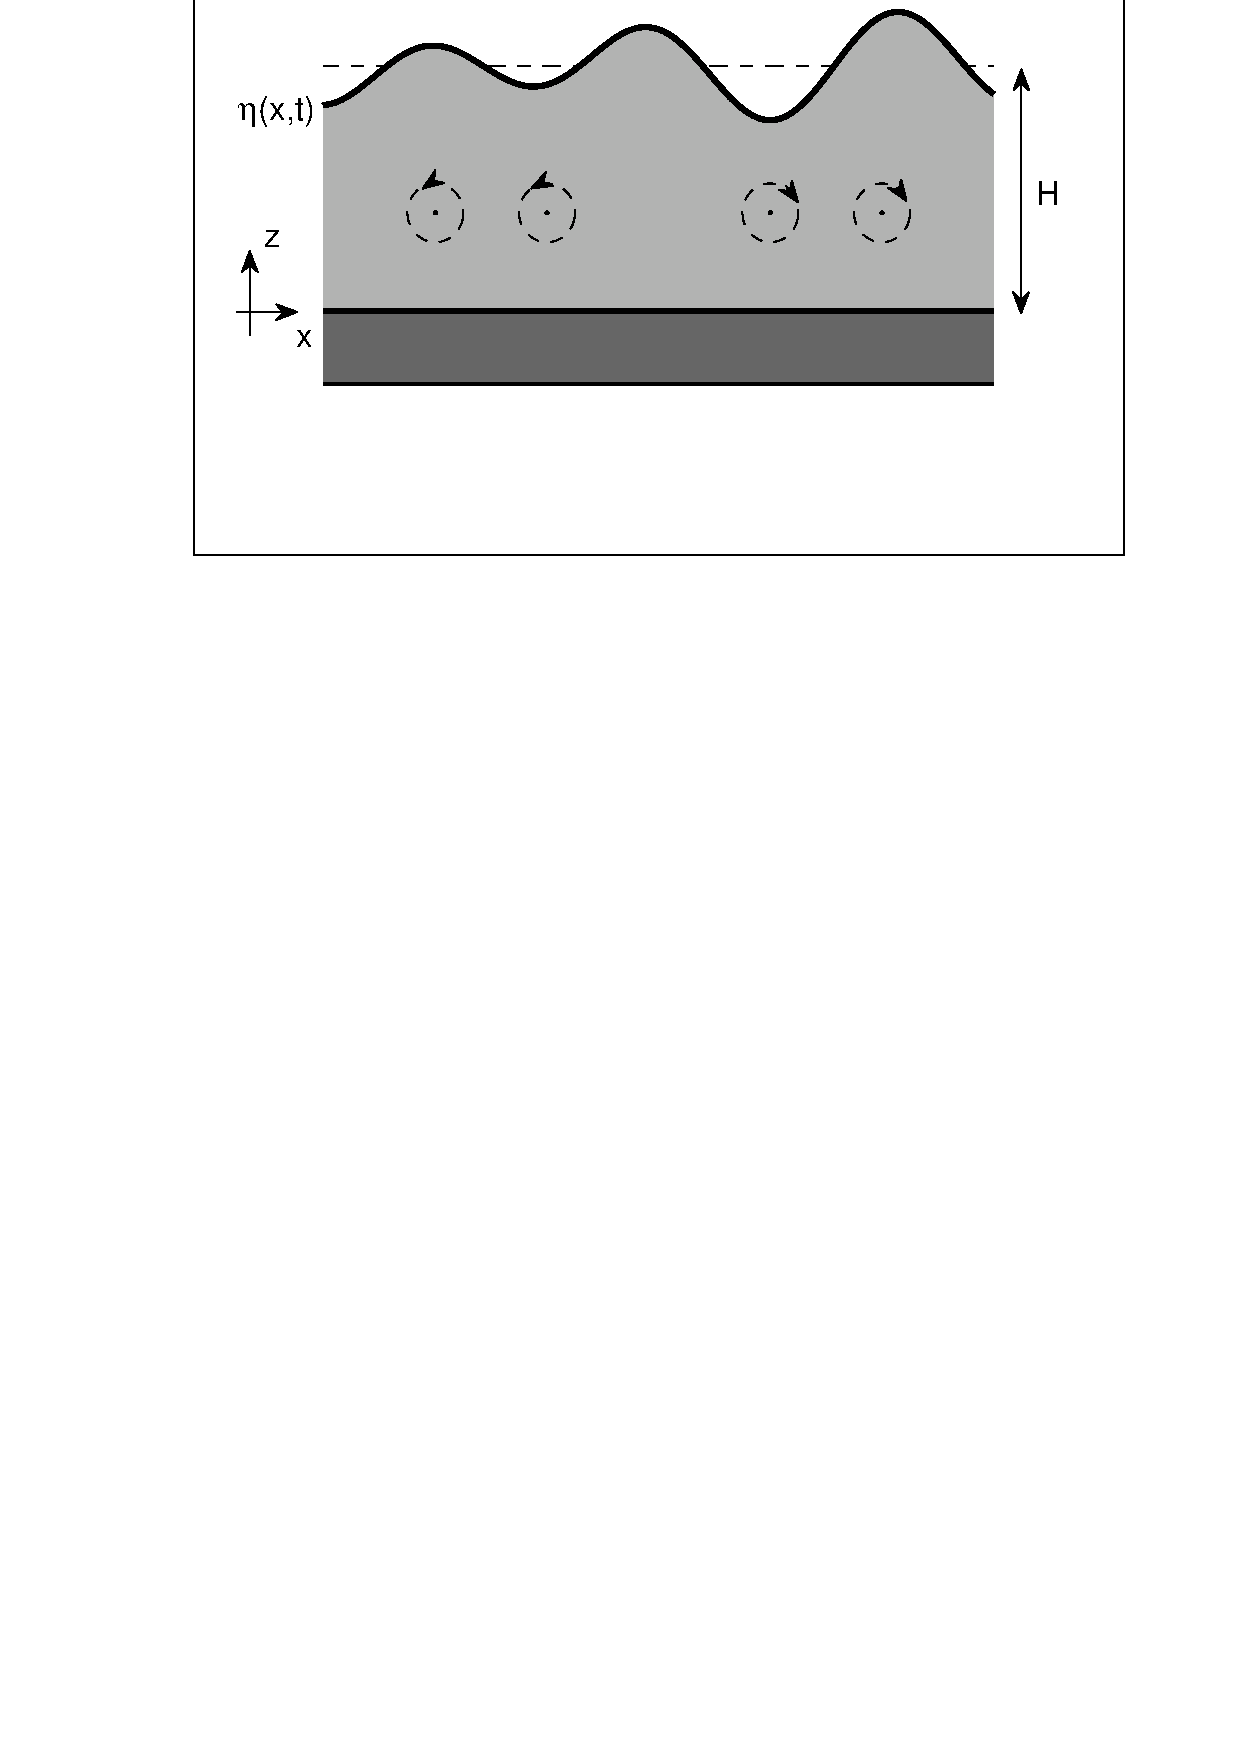
\includegraphics[width=0.5\textwidth]{CurtisKalisch_Vortices}
\caption{\small Irrotational point vortices submerged under a free surface gravity wave.}
\label{fig:vortex}
\end{figure}

Given our assumptions on the fluid, the fluid velocity ${\bf u}$ is given by the gradient of a potential, say $\phi$.  We can further separate this potential by writing 
\[
\phi(x,z,t) = \phi_{v}(x,z,t) + \tilde{\phi}(x,z,t).
\]
The potential $\tilde{\phi}$ describes the bulk and surface fluid flow while the potential describing the vortex motion, $\phi_{v}$, is defined to be
\begin{equation}
\phi_{v}(x,z,t) = \frac{1}{2\pi}\sum_{j=1}^{N}\Gamma_{j} \phi_{v,j}(x,z,t),
\label{vortpoten}
\end{equation}
with $\Gamma_{j}$ denoting the circulation strength of the vortices and
\[
\phi_{v,j}(x,z,t) = \phi_{v,j}^{+}(x,z,t) - \phi_{v,j}^{-}(x,z,t), 
\]
where, denoting the vortex positions as ${\bf x}_{j}(t) = \left(x_{j}(t),z_{j}(t)\right)$, we set 
\[
\phi_{v,j}^{+}(x,z,t) = \Phi_{p}(x-x_{j}(t),z-z_{j}(t)), ~ \phi_{v,j}^{-}(x,z,t) = \Phi_{p}(x-x_{j}(t),z+z_{j}(t)), 
\]
where
\[
\Phi_{p}(x,z) = \sum_{m=-\infty}^{\infty} \tan^{-1}\left(\frac{z}{x-2m L} \right).
\]
Our choice for $\phi_{v}$, aside from addressing the requirement of periodic boundary conditions, ensures that 
\[
\left.\p_{z}\phi_{v}\right|_{z=0} = 0.
\]
By further supposing that 
\[
\left.\p_{z}\tilde{\phi}\right|_{z=0} = 0, 
\]
we satisfy the assumption that $z=0$ is an impermeable boundary.  

%While we should think of the sum defining $\phi_{v}$ formally, this is not the case for its derivatives, which ultimately define the physically meaningful fluid velocity.  
% Using Fourier transform arguments, one can show that 
%\[
%\sum_{m=-\infty}^{\infty}\frac{s}{(t-2m\pi)^{2}+s^{2}} = \frac{\sinh(s)}{2(\cosh(s)-\cos(t))}
%\]
%and
%\[
%\sum_{m=-\infty}^{\infty}\frac{t-2m\pi}{(t-2m\pi)^{2}+s^{2}} = \frac{\sin(t)}{2(\cosh(s)-\cos(t))}
%\]
Standard arguments then give for the vortex velocities
\begin{align}
\dot{x}_{j} = & \frac{1}{4L}\left(  \Gamma_{j}\mbox{cotanh}\left(\frac{\pi z_{j}}{L} \right)+2\sum_{l\neq j}\Gamma_{l}v_{jl}^{(h)} \right)+ \tilde{\phi}_{x}(x_{j},z_{j},t),\label{xveloc}\\
\dot{z}_{j} = & \frac{1}{2L}\sinh\left(\frac{\pi}{L}z_{j}\right)\sum_{l\neq j} \Gamma_{l} v_{jl}^{(v)} + \tilde{\phi}_{z}(x_{j},z_{j},t),\label{zveloc}
\end{align}
where
\begin{align*}
v_{jl}^{(h)} = & \frac{\sinh\left(\frac{\pi}{L}z_{l}\right)\left(\cosh(\frac{\pi}{L}z_{l})-\cosh(\frac{\pi}{L}z_{j})\cos\left(\frac{\pi}{L}(x_{j}-x_{l})\right)\right)}{\left(\cosh\left(\frac{\pi}{L}(z_{j}-z_{l})\right)-\cos\left(\frac{\pi}{L}(x_{j}-x_{l})\right)\right)\left(\cosh\left(\frac{\pi}{L}(z_{j}+z_{l})\right)-\cos\left(\frac{\pi }{L}(x_{j}-x_{l})\right)\right)}, \\
v_{jl}^{(v)} = & \frac{\sin\left(\frac{\pi}{L}(x_{j}-x_{l})\right)\sinh\left(\frac{\pi}{L}z_{l}\right)}{\left(\cosh\left(\frac{\pi}{L}(z_{j}-z_{l})\right)-\cos\left(\frac{\pi}{L}(x_{j}-x_{l})\right)\right)\left(\cosh\left(\frac{\pi}{L}(z_{j}+z_{l})\right)-\cos\left(\frac{\pi }{L}(x_{j}-x_{l})\right)\right)}.
\end{align*}
At the surface, we have the kinematic condition which, separating into vortex and bulk variables becomes 
\begin{equation}
\eta_{t} - \tilde{\phi}_{z} + \eta_{x}\tilde{\phi}_{x} =  P_{v}(x,\eta,t), ~ z =  \eta(x,t)+H,  
\label{unsckin}
\end{equation}
where
\[
P_{v}(x,\eta,t) =   \p_{z}\phi_{v} -  \eta_{x}\p_{x}\phi_{v} .
\]
Finally, at the surface, we have the Bernoulli equation, which becomes after separating into vortex and bulk variables  
\begin{equation}
\tilde{\phi}_{t} + \frac{1}{2 }\left| \nabla \tilde{\phi} \right|^{2} +  \nabla\phi_{v}\cdot \nabla\tilde{\phi} + g\eta = E_{v}(x,\eta,t),
\label{unscbern}
\end{equation}
where
\[
E_{v}(x,\eta,t) = \frac{1}{2\pi}\sum_{j=1}^{N}\Gamma_{j}\left(\dot{x}_{j}\p_{x}\phi_{v,j} + \dot{z}_{j} \p_{z}\left(\phi_{v,j}^{+} + \phi_{v,j}^{-}\right)  \right) - \frac{1}{2}\left| \nabla \phi_{v} \right|^{2}.
\]
The system given by Equations \eqref{xveloc}-\eqref{unscbern} coupled with the bulk requirement that 
\begin{equation}
\Delta \tilde{\phi} = 0, ~ 0\leq z \leq \eta(x,t)+H,
\label{harmon} 
\end{equation}
and the Neumann boundary condition $\p_{z}\tilde{\phi}(x,0,t)=0$, gives a closed system of equations in terms of $\eta$, $\tilde{\phi}$, and the vortex positions $(x_{j}(t),z_{j}(t))$.  However, this requires the solution of a nonlinear free boundary value problem, which does not allow for any direct analytic solution approaches.  Further, even with regards to developing numerical schemes, any method which removes the need to solve throughout the bulk of the fluid is desirable.
This goal can be at least partially achieved by defining 
\[
\tilde{q}(x,t) = \tilde{\phi}(x,\eta(x,t)+H,t).
\]
We can then transform the derivatives of the potential at the surface via the equations
\begin{equation}
\left.\bp\tilde{\phi}_{x}\\ \tilde{\phi}_{z}\ep\right|_{z=\eta + H} = \frac{1}{1+\eta_{x}^{2}}\bp 1 & \eta_{x}\\ \eta_{x} & -1\ep\bp\tilde{q}_{x} \\  -\eta_{t} + P_{v}\ep,
\label{phitrans}
\end{equation}
and
\begin{equation}
\tilde{\phi}_{t} = \tilde{q}_{t}-\tilde{\phi}_{z}\eta_{t}.
\label{phittrans}
\end{equation}
In this way, it is possible to rewrite the Bernoulli equation \eqref{unscbern} in terms of surface variables and vortex positions alone.  However, since we have made use of the kinematic condition Equation \eqref{unsckin}, we cannot rewrite this equation in terms of itself.  Likewise, we have no means of removing the bulk-variable dependence in Equations \eqref{xveloc} and \eqref{zveloc}.

To address this issue, we now turn to the method of Ablowitz, Fokas, and Musslimani (AFM) as described in \cite{afm}.  Through an extension to the existing scheme, we will be able to write a closed system of equations in terms of surface variables and vortex positions alone.  This will remove any need to solve equations, either analytically or numerically, throughout the bulk of the fluid.  As we show, this approach then readily allows us to derive efficient numerical approximation schemes.

%%%%%%%%%%%%%%%%%%%%%%%%%%%%%%%%%%%%%%%%%%%%%%%%%%%%%%%%%%%%%%%%%%%%%%%%%%%%%%
\section{The Surface-Variable/Vortex-Position Formulation}
We now show how to rewrite the system of equations \eqref{xveloc}-\eqref{harmon} in terms of surface variables and vortex positions alone via the method described in \cite{afm}.  Making use of Equation \eqref{unsckin}, the work in \cite{afm} readily allows us to rewrite the kinematic condition as the infinite system of integro-differential equations  
\begin{equation}
\int_{-L}^{L} e^{-i\pi k x/L}\left(\cosh( k(\eta+H))\left(\eta_{t} - P_{v} \right) + i\tilde{q}_{x}\sinh(k( \eta+H))\right) dx = 0, \label{unscafm}
\end{equation}
for $k \in \mathbb{Z}\backslash\left\{0\right\}$.  We omit the details of this derivation since one may directly follow the arguments in \cite{afm} to derive \eqref{unscafm}.

Looking at Equations \eqref{xveloc} and \eqref{zveloc} though, we are still left with needing to evaluate the background flow potential $\tilde{\phi}$ at the vortex positions $\left(x_{j}, z_{j}\right)$.  To deal with this, we introduce the auxiliary harmonic functions 
\[
\psi_{j}(x,z,t) = - \frac{1}{4\pi}\sum_{m=-\infty}^{\infty} \left( \mbox{ln}\left( \tilde{x}_{j,m}^{2} + \tilde{z}_{j,-}^{2}  \right) + \mbox{ln}\left( \tilde{x}_{j,m}^{2} + \tilde{z}_{j,+}^{2} \right)\right).
\]
where
\[
\tilde{x}_{j,m} = \frac{(x-x_{j}-2mL)}{L}, ~ \tilde{z}_{j,-} = \frac{\gamma}{H}(z-z_{j}), ~ \tilde{z}_{j,+} = \frac{\gamma}{H}(z+z_{j}),
\]
and
\[
\gamma = \frac{H}{L}.
\]
We are then able to show the identity
\[
\tilde{\phi}_{x}(x_{j},z_{j},t) = -\int_{-L}^{L} \left.\left(\tilde{\phi}_{z}\left(\p_{x}\psi_{j}+ \eta_{x}\p_{z}\psi_{j}\right)+\tilde{\phi}_{x}\left(-\eta_{x}\p_{x}\psi_{j} + \p_{z}\psi_{j} \right) \right)\right|_{z=\eta+H}dx,
\]
See the Appendix, Section \ref{deriv}, for the technical details of the derivation.  Using the kinematic condition and basic definitions then allows us to show that 
\begin{equation}
\tilde{\phi}_{x}(x_{j},z_{j},t) = -\int_{-L}^{L}\left.\left(\left(\eta_{t}-P_{v}\right)\p_{x}\psi_{j} + \tilde{q}_{x}\p_{z}\psi_{j} \right) \right|_{z=\eta+H} dx.
\label{blkeq}
\end{equation}

Proceeding in a similar fashion for $\tilde{\phi}_{z}$, we introduce the auxiliary harmonic function
\[
\tilde{\psi}_{j} = -\frac{1}{4\pi}\sum_{m=-\infty}^{\infty} \left( \mbox{ln}\left( \tilde{x}_{j,m}^{2} + \tilde{z}_{j,-}^{2}  \right) - \mbox{ln}\left( \tilde{x}_{j,m}^{2} + \tilde{z}_{j,+}^{2} \right)\right).
\]
This choice ensures that $\tilde{\psi}_{j}(x,0,t) = 0$.  Again, using the arguments described in the Appendix, Section \ref{deriv}, we then can find that
\[
\tilde{\phi}_{z}(x_{j},z_{j},t) = -\int_{-L}^{L}\left.\left( \tilde{\psi}_{j}\left(\eta_{x}\tilde{\phi}_{xz}+\tilde{\phi}_{xx}\right)+\tilde{\phi}_{z}\left(-\eta_{x}\p_{x}\tilde{\psi}_{j}+\p_{z}\tilde{\psi}_{j}\right) \right)\right|_{z=\eta+H} dx.
\]
Again, the kinematic condition and basic definitions then allows us to show that
\[
\tilde{\phi}_{z}(x_{j},z_{j},t) = -\int_{-L}^{L}\left.\left( \left(\eta_{t}-P_{v}\right)\p_{z}\tilde{\psi}_{j} - \tilde{q}_{x}\p_{x}\tilde{\psi}_{j} \right)\right|_{z=\eta+H} dx.
\]
Thus, we have now shown how to rewrite Equations \eqref{xveloc} and \eqref{zveloc} in the bulk-independent form 
\begin{align}
\dot{x}_{j} = & \frac{1}{4L}\left(  \Gamma_{j}\mbox{cotanh}\left(\frac{\pi z_{j}}{L} \right)+2\sum_{l\neq j}\Gamma_{l}v_{jl}^{(h)} \right)\nonumber\\
&  -\int_{-L}^{L}\left.\left(\left(\eta_{t}-P_{v}\right)\p_{x}\psi_{j} + \tilde{q}_{x}\p_{z}\psi_{j} \right)\right|_{z=\eta + H} dx, \label{xdotb}\\
\dot{z}_{j} = &  \frac{1}{2L}\sinh\left(\frac{\pi}{L}z_{j}\right)\sum_{l\neq j} \Gamma_{l} v_{jl}^{(v)}\nonumber\\
& - \int_{-L}^{L}\left.\left( \left(\eta_{t}-P_{v}\right)\p_{z}\tilde{\psi}_{j} - \tilde{q}_{x}\p_{x}\tilde{\psi}_{j} \right)\right|_{z=\eta + H} dx. \label{zdotb}
\end{align}
Thus, coupled with the use of \eqref{phitrans} to rewrite \eqref{unscbern}, and the use of the AFM method to derive \eqref{unscafm}, we have now derived a system of equations that are in terms of surface variables and vortex positions alone.  
%The approach outlined above complements those used for particle tracing in \cite{kalisch} and \cite{nachbin}.  
%%%%%%%%%%%%%%%%%%%%%%%%%%%%%%%%%%%%%%%%%%%%%%%%%%%%%%%%%%%%%%%%%%%%%%%%%%%%%%%%
\section{Scalings, Numerical Implementation, and Linear Dynamics}
We now choose the following non-dimensionalizations 
\[
\tilde{x} = \frac{x}{L}, ~\tilde{z} = \frac{z}{H}, ~ \tilde{t} = \frac{\sqrt{gH}}{L} t, ~ \eta = d\tilde{\eta}, ~ \tilde{\phi} = \mu L\sqrt{gH} \tilde{\tilde{\phi}}, ~ \tilde{\Gamma}_{j} = \frac{\Gamma_{j}}{\Gamma},
\]
where we define the non-dimensional parameters
\[
\mu= \frac{d}{H}, ~ \gamma = \frac{H}{L},
\]
and where we define the Froude number $F$ to be 
\[
F = \frac{\Gamma}{\mu L \sqrt{gH}}.
\]
Recall that $L$ is the length of the domain, and note that $d$ is taken as the expected amplitude of the free surface.  These scalings are motivated mainly by the goal of obtaining an efficient numerical procedure.  If we then define $Q = \tilde{q}_{x}$, the Bernoulli equation \eqref{unscbern} becomes, after using Equations \eqref{phitrans} and \eqref{phittrans} and then dropping tildes,  
\begin{multline}
Q_{t} + \eta_{x} + \mu\p_{x}\frac{1}{1+ \mu^{2}\gamma^{2}\eta_{x}^{2}} \left( \frac{1}{2}Q^{2} - \mu \gamma^{2}\eta_{t}\eta_{x}Q  +  \phi_{sx} (Q + \mu\gamma\eta_{x}( P_{s}-\gamma\eta_{t}))   \right. \\
\left. + \frac{1}{2}\left(P_{s}^{2}-\gamma^{2}\eta_{t}^{2} \right)+ \phi_{sz}\left(\gamma \mu \eta_{x}Q-\left(P_{s}-\gamma \eta_{t}\right) \right) \right)= \p_{x}E_{s}(x,t), \label{swbern}
\end{multline}
where 
\[
P_{s}(x,t) = \phi_{sz}(x,t)-\mu\gamma \eta_{x}\phi_{sx}(x,t),
\]
and
\begin{align*}
E_{s}(x,t) =  F\sum_{j=1}^{N}\Gamma_{j}\left(\dot{x}_{j}\varphi_{x}(x-x_{j},1+\mu\eta;z_{j}) + \gamma\dot{z}_{j}\tilde{\varphi}_{z}(x-x_{j},1+\mu\eta;z_{j}) \right)
& -\frac{\mu}{2}\left(\phi_{sx}^{2} + \phi_{sz}^{2}\right).
\end{align*}
The AFM equation \eqref{unscafm} becomes  
\begin{multline}
\int_{-1}^{1} e^{-i\pi k x}\left(\cosh\left( \pi\gamma k (1 + \mu \eta)\right)\left(\eta_{t} - \frac{1}{\gamma}P_{v}(x,1+\mu\eta,t) \right) \right.\\
\left.+i  \frac{1}{\gamma}Q\sinh\left(\pi \gamma k (1 + \mu \eta)\right)\right) dx = 0,~k\in\mathbb{Z},\label{finafm}
\end{multline}
and Equations \eqref{xdotb} and \eqref{zdotb} become
\begin{align}
\dot{x}_{j} = &\frac{F\mu}{4}\left(\Gamma_{j}\mbox{cotanh}\left(\pi \gamma z_{j} \right)+2\sum_{l\neq j}\Gamma_{l}v_{jl}^{(h)} \right)+\label{scxveloc}\\
& \mu \int_{-1}^{1} \left.\left( \left(\gamma \eta_{t}-P_{s} \right) \tilde{\varphi}_{z}(x-x_{j},z;z_{j}) +  Q \tilde{\varphi}_{x}(x-x_{j},z;z_{j}) \right)\right|_{z=1+\mu\eta} dx, \nonumber\\
\dot{z}_{j} = & \frac{F\mu}{2\gamma}\sinh\left( \pi \gamma z_{j}\right)\sum_{l\neq j} \Gamma_{l} v_{jl}^{(v)}-\label{sczveloc}\\
&  \frac{\mu}{\gamma }\int_{-1}^{1} \left.\left(\left(\gamma \eta_{t}-P_{s}\right) \varphi_{x}(x-x_{j},z;z_{j}) + Q \varphi_{z}(x-x_{j},z;z_{j}) \right)\right|_{z=1+\mu\eta}dx, \nonumber
\end{align}
The definitions of $\phi_{sx}$, $\phi_{sz}$, $\varphi_{x}$, $\varphi_{z}$, $\tilde{\varphi}_{x}$, and $\tilde{\varphi}_{z}$ can be found in the Appendix, Section \ref{poterms},.  We now develop the machinery necessary to implement numerical schemes to solve the system of equations \eqref{swbern}, \eqref{finafm}, \eqref{scxveloc}, and \eqref{sczveloc}.  
%%%%%%%%%%%%%%%%%%%%%%%%%%%%%%%%%%%%%%%%
\subsection{Dirichlet-to-Neumann Expansions}
%%%%%%%%%%%%%%%%%%%%%%%%%%%%%%%%%%%%%%%%
Our choice of scaling allows us to readily generate the Dirichlet-to-Neumann Operator (DNO) expansion.  This is done, as in \cite{craig} and elsewhere, by supposing that 
\[
\eta_{t} - \frac{1}{\gamma}P_{v}(x,1+\mu \eta,t) = \left(G_{0} + \mu G_{1} + \mu^{2}  G_{2} + \cdots \right)Q.
\]
Defining the Fourier transform of a periodic function $f(x)$ to be $\hat{f}$, so that 
\[
\hat{f}(k) = \frac{1}{2}\int_{-1}^{1}f(x)e^{-i\pi k x} dx, ~ k\in \mathbb{Z},
\]
we define, for a linear operator $L$, its associated symbol $\hat{L}(k)$ by way of the formula 
\[
\hat{L}(k)\hat{f}(k) = \frac{1}{2}\int_{-1}^{1} Lf(x) e^{-i\pi k x}dx.
\]
Using the AFM equation \eqref{finafm}, we then get 
\[
\hat{G}_{0}(k) = -\frac{i}{\gamma}\tanh(\pi \gamma k),
\]
and, for $m\geq 1$, 
\begin{align*}
G_{m}Q = & -\sum_{j=1}^{\lfloor{m/2}\rfloor}\frac{1}{(2j)!}D^{2j}_{\gamma}\left(\eta^{2j}G_{m-2j}Q\right) \\
& - \gamma^{2}\p_{x}G_{0} \sum_{j=0}^{\lfloor{(m-1)/2}\rfloor}\frac{D_{\gamma}^{2j}}{(2j+1)!}\left(\eta^{2j+1}G_{m-2j-1}Q\right) - \frac{1}{m!}L_{m} \p_{x}D_{\gamma}^{m-1}\left(\eta^{m}Q \right),
\end{align*}
where
\[
\hat{D}_{\gamma} = \pi \gamma k,
\]
and
\[
\hat{L}_{m} = \left\{
\ba{rl}
1,  & m~\mbox{is odd}, \\
i\gamma \hat{G}_{0}(k),  & m~\mbox{is even}.
\ea
\right.
\]

In order to build a numerical method though, there is of course the question of where to truncate the DNO expansions.  Throughout the paper, we use the convention of taking enough terms, say $\tilde{N}$, such that, using the numerically computed solution for $Q(x,t_{f})$, we satisfy the criteria  
\begin{equation}
\frac{\gnorm{G_{\tilde{N}} Q(\cdot,t_{f})}_{2}}{\gnorm{Q(\cdot,t_{f})}_{2}} \leq \mbox{eps},
\label{trunccond}
\end{equation}
where $\mbox{eps}$ denotes machine precision, which on 64-bit machines is on the order of $10^{-16}$.  Here, $t_{f}$ is the final time to which a given simulation is run.  We argue that satisfying this inequality should in most cases imply subsequent terms should have little to no effect on the dynamics.  For each simulation presented in this paper, by choosing multiple truncation points, no effect was seen by including terms beyond what would be selected via our truncation convention.
%%%%%%%%%%%%%%%%%%%%%%%%%%%%%%%%%%%%%%%%
\subsection{Linear Dynamics}
%%%%%%%%%%%%%%%%%%%%%%%%%%%%%%%%%%%%%%%%
In order to get at least some short time intuition about the response of the above system, we suppose that $\mu \ll \gamma$, so that in the linear regime we have $\dot{x}_{j}\sim 0$, $\dot{z}_{j}\sim 0$, 
\[
Q_{t} + \eta_{x} = 0,
\]
and
\[
\hat{\eta}_{t} -\hat{G}_{0}(k)\hat{Q} = F\int_{\mathbb{R}}e^{-i \pi kx} \tilde{P}_{v}dx,
\]
where
\[
\tilde{P}_{v} = \frac{\gamma\sqrt{2}}{\pi}\sum_{j=1}^{n}\Gamma_{j}z_{j}e^{-i\pi kx_{j}} \frac{x}{(x^{2}+\gamma^{2}(1-z_{j})^{2})(x^{2}+\gamma^{2}(1+z_{j})^{2})} .
\]
We can readily show using a contour integral argument that 
\[
\int_{\mathbb{R}}e^{-i\pi kx} \tilde{P}_{v}dx = -\frac{i}{\sqrt{2}}\sum_{j=1}^{n}\Gamma_{j} \frac{\sinh(\pi \gamma k z_{j})}{\gamma} e^{-i\pi kx_{j}-\pi \gamma |k|}. 
\]
Note, in order for this result to hold, we need to assume that $0\leq z_{j} <1$.  Thus, if we linearize around a quiescent initial condition, using \eqref{vortpoten} whereby we have
\[
\hat{\eta}(k,0)=0, ~ \hat{Q}(k,0)=\hat{Q}_{0}(k) = -ik\hat{\phi}_{v}(k,1)
\]
in frequency space, we get the leading order behavior
\begin{align*}
\bp \hat{Q}(k,t) \\ \hat{\eta}(k,t) \ep = & \hat{Q}_{0}(k)\bp \cos(\omega(k)t)\\\frac{ \omega}{i\pi k} \sin(\omega(k)t)\ep \\
&-\frac{iF}{\sqrt{2}}\bp i\pi k(\cos(\omega(k)t)-1)/\omega(k) \\   \sin(\omega(k)t) \ep \sum_{j=1}^{n}\Gamma_{j}\frac{\sinh(\pi \gamma k z_{j})}{\gamma \omega(k)}e^{-i\pi kx_{j}-\pi \gamma |k|},
\end{align*}
where 
\[
\omega(k) = \sqrt{\frac{ \pi k \tanh(\pi \gamma k)}{ \gamma }}.  
\]
Defining the surface response to the vortex induced forcing as $R_{s}(x,t)$, we readily see that this is given by 
\[
R_{s}(x,t) = F\sum_{j=1}^{n}\Gamma_{j}R_{s,j}(x,t).
\]
where the functions $R_{s,j}$ are found by taking inverse Fourier transforms and using symmetry arguments such that one finds  
\begin{equation}
R_{s,j}(x,t) = \sum_{k=1}^{\infty} \frac{\sin(\omega(k)t)}{\omega(k)}\frac{\sinh(\pi \gamma k z_{j})}{\gamma}e^{-\pi \gamma k}\sin(\pi k (x-x_{j})).
\label{surfresp}
\end{equation}

%%%%%%%%%%%%%%%%%%%%%%%%%%%%%%%%%%%%%%%%
\subsection{Convergence of the method for $F=0$}

In order to test our numerical method and the formulation of the problem, we take $F=0$ and use initial conditions corresponding to the choice $t=0$ in the solutions to the KdV Equation given in the next section by Equations \eqref{kdvsolpot} and \eqref{kdvsolsurf} with $\tilde{m}=0.2$ and $q_{0}$ chosen so that the initial conditions have zero spatial average.  While KdV solutions are not exact, we provide a Cauchy convergence study of our method to establish its validity throughout the remainder of the paper.  For all of the following simulations, we use a pseudo-spectral in space and a fourth order Runge-Kutta time-integration scheme. 
The time step used is $\delta t = 1\times 10^{-2}$, and the error introduced by these choices is on the order of $10^{-8}$.  In order to avoid aliasing, the Orszag ``2/3-rule'' is used throughout the simulations. 

The chief concern with regards to numerical accuracy in using DNO expansions comes from issues related to the catastrophic cancellation of the higher order terms \cite{wilkening}. To see this, we first choose $\mu=0.2$, $\gamma=\sqrt{\mu}$, and the final time of the simulation $t_{f}=12$.  We choose $K_{M}=256$ and $K_{M}=512$, and we truncate the DNO expansion at the 11th term $\tilde{N}=10$ for both choices of $K_{M}$; see Equation \eqref{trunccond} for reference.  We see in Figure \ref{fig:convcomp} that the two solutions for $\eta(x,12)$ are indistinguishable up to machine precision.  We note that this result has nothing to do with the validity of KdV as an approximation to the full problem.  We therefore see over an asymptotically significant time scale, i.e. $t_{f} > 2/\mu$, that the method has converged in the Cauchy sense.    
\begin{figure}[h]
\centering
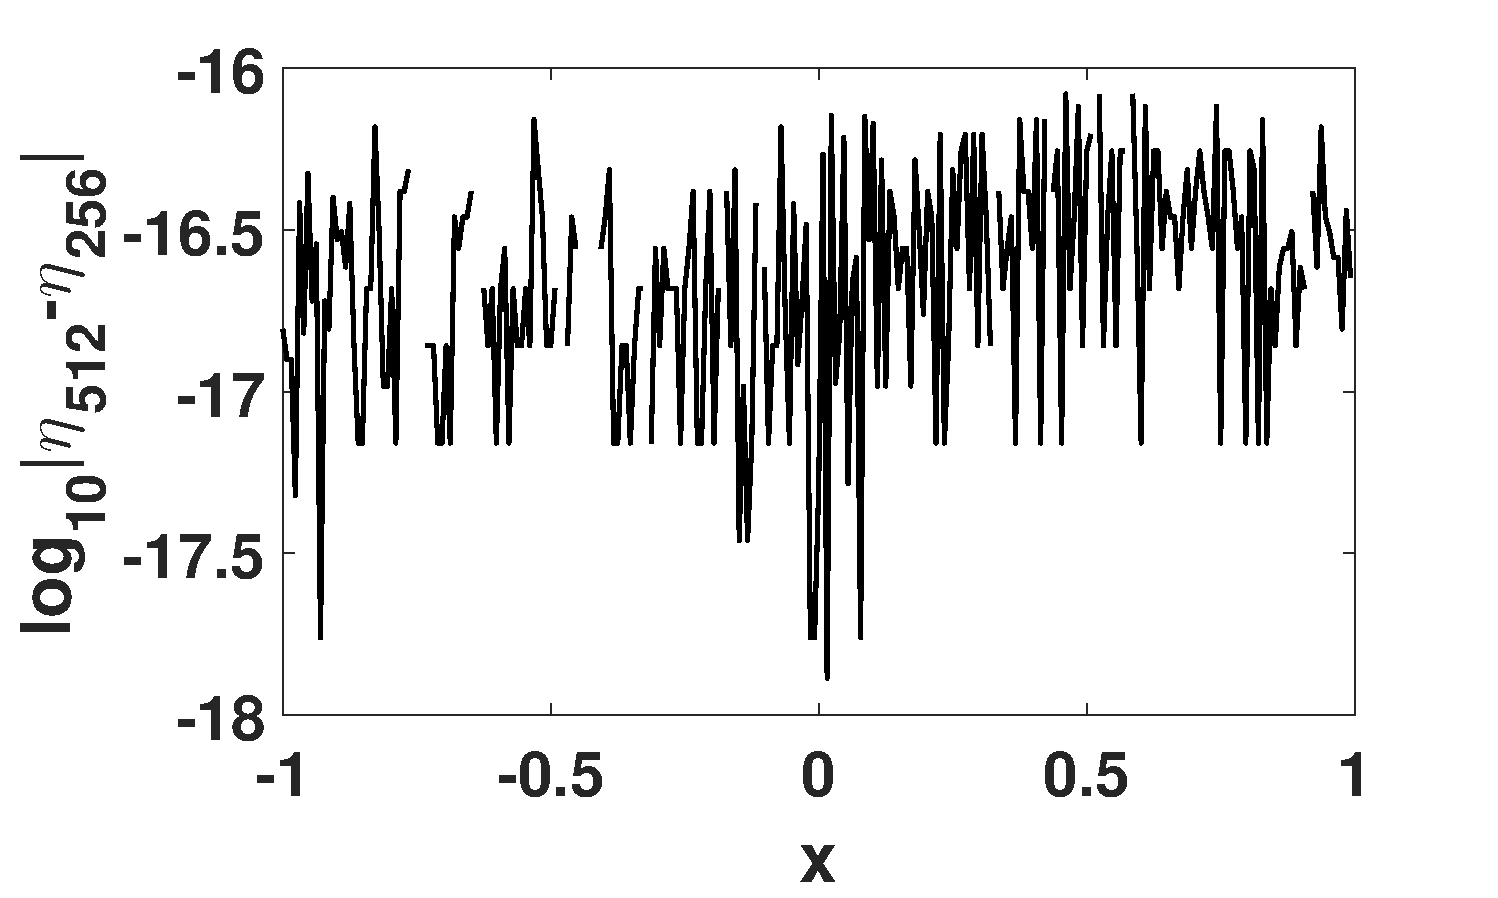
\includegraphics[width=0.48\textwidth]{conv_plot_tf_12}
\caption{The log plot of the difference in the solutions at $t_{f} = 12$ using $K_{M}=256$ and $K_{M}=512$ modes.  As can be seen, the solutions are identical up to machine precision, and thus the sampling rate described in the introduction should be sufficient.  Here $\mu=0.2$ and $\gamma=\sqrt{\mu}$.}
\label{fig:convcomp}
\end{figure}

In contrast, we now choose $\mu=0.4$ while still letting $\gamma=\sqrt{\mu}$.  Again letting $t_{f} =12$, we compare the performance of the method by looking at the difference between using $K_{M}=64$ and $K_{M}=128$ modes and then using $K_{M}=256$ and $K_{M}=512$ modes.  We double the number of terms used in the DNO expansion by truncating at the 21st mode $\tilde{N}=20$.  As seen in the left panel of Figure \ref{fig:convcompfail}, while one can argue that using $K_{M}=512$  modes still produces a very accurate solution, the combination of the larger value of $\mu$ and $\gamma$ has allowed for the catastrophic cancellation described in \cite{wilkening} to begin to drive errors up in comparison to using simulations with lower numbers of modes.   
\begin{figure}[h]
\centering
\begin{tabular}{cc}
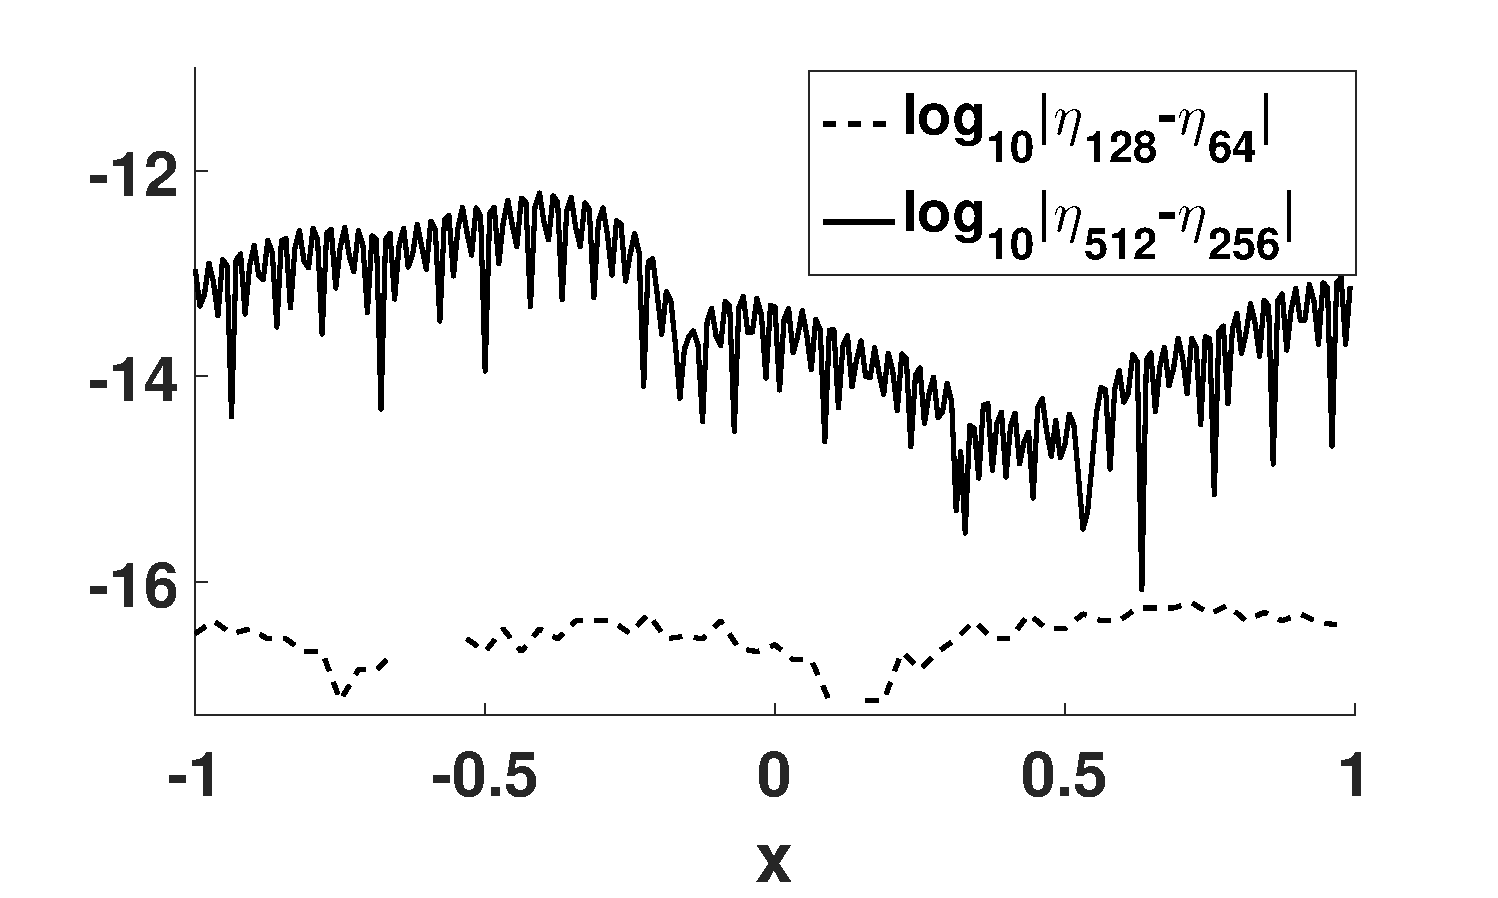
\includegraphics[width=0.48\textwidth]{conv_plot_mupt4_tf_12} & 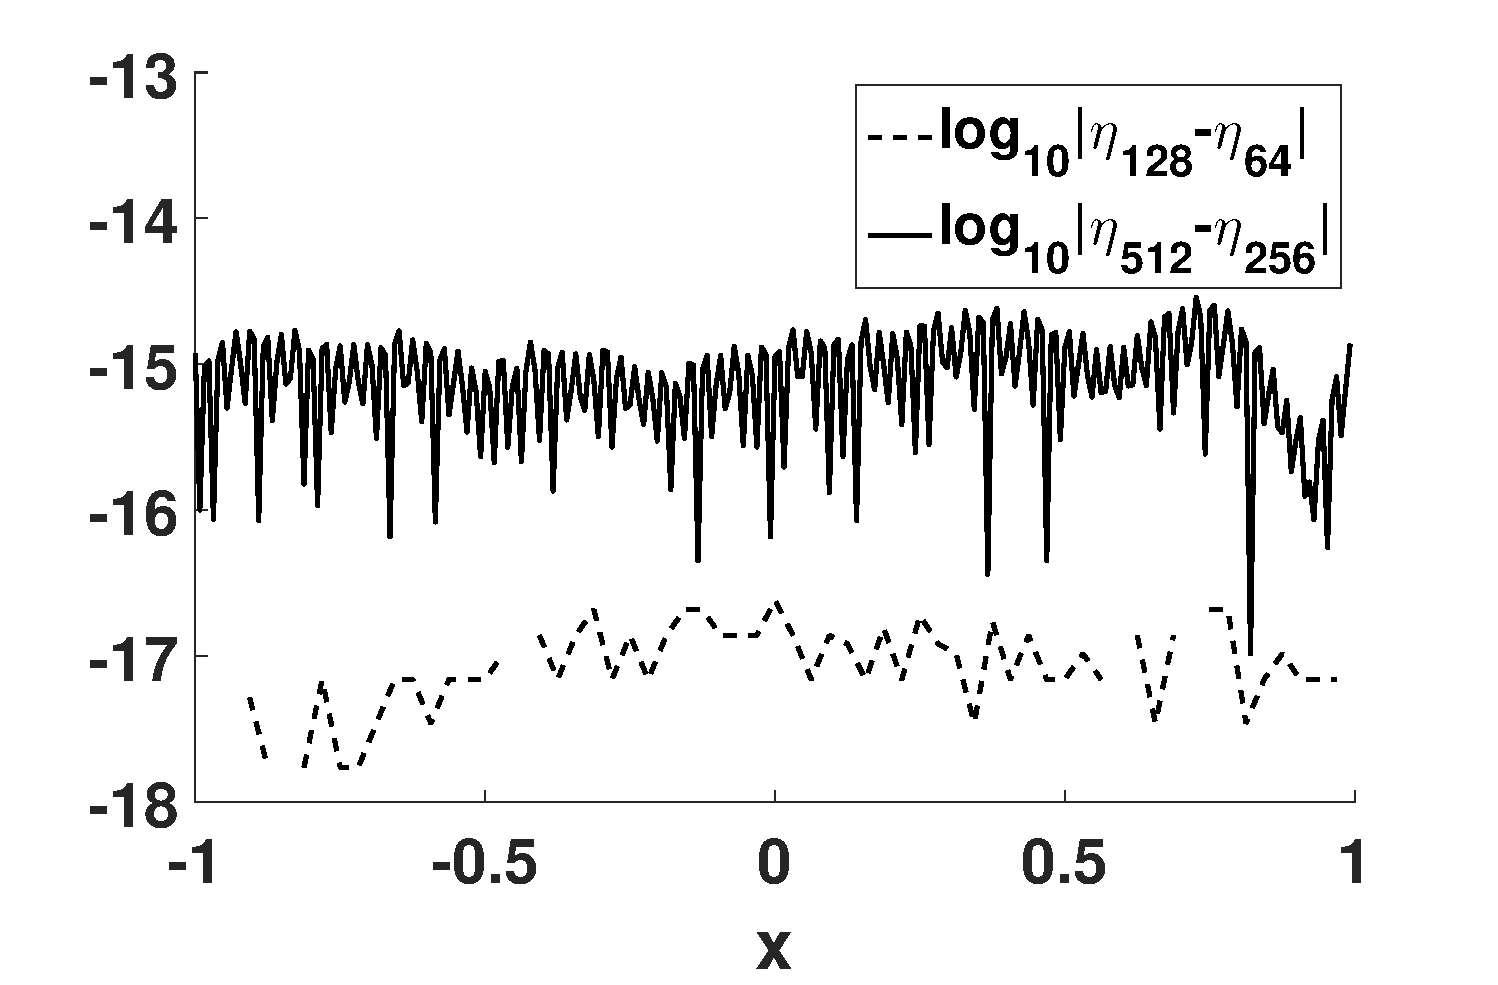
\includegraphics[width=0.48\textwidth]{conv_plot_mupt4_gampt4_tf_12}
\end{tabular}
\caption{ Left Panel: For $\mu=0.4$ and $\gamma=\sqrt{\mu}$, the log plot of the difference in the solutions at $t_{f}=12$ using $K_{M}=64$ and $K_{M}=128$ modes (- -) and using $K_{M}=256$ and $K_{M}=512$ modes (-).  The introduction of higher modes allows catastrophic cancellation to remove two digits of accuracy. Right Panel: For $\mu=0.4$ and $\gamma=\mu$, the log plot of the difference in the solutions at $t_{f}=12$ using $K_{M}=64$ and $K_{M}=128$ modes (- -) and using $K_{M}=256$ and $K_{M}=512$ modes (-). While catastrophic cancellation still plays a role, by decreasing the magnitude of $\gamma$, it is significantly mitigated.}
\label{fig:convcompfail}
\end{figure}
To further make the point, we can reduce the magnitude of the long wave parameter $\gamma$ such that $\gamma=\mu=0.4$.  In this case, as we see in the right panel of Figure \ref{fig:convcompfail}, while catastrophic cancellation issues still keep the simulations with $K_{M}=512$ modes as accurate as lower mode simulations, this effect is greatly mitigated by having reduced the magnitude of the long wavelength parameter $\gamma$.

%%%%%%%%%%%%%%%%%%%%%%%%%%%%%%%%%%%%%%%%%%%%%%%%%%%%%%%%%%%%%%%%%%%%%%%%%%%%%%%%
\section{Numerical Results}
%%%%%%%%%%%%%%%%%%%%%%%%%%%%%%%%%%%%%%%%%%%%%%%%%%%%%%%%%%%%%%%%%%%%%%%%%%%%%%%%

We now describe the general details of our numerical experiments involving different vortex configurations.  Throughout the remainder of the paper, while our choice for $\mu$ will vary, we choose $\gamma = \sqrt{\mu}$ since this corresponds to the KdV balance described above and is a typical choice for ``shallow-water'' models.  This scaling is chosen here because it is in the shallow-water regime that the finite depth is felt most acutely.  Based on the convergence studies above, we likewise sample the domain with $K_{M} = 512$ modes so that the wavenumbers $k$ satisfy $-255\leq k \leq 256$.  Again, the Orszag ``2/3-rule'' is used throughout the simulations.  Thus, since the non-dimensional domain is $[-1,1]$, this choice corresponds to a grid spacing of $\delta x \approx 0.006$.  

For the problems involving only two vortices, we use the initial horizontal positions
\begin{equation}
x_{1}(0)=-\mu\gamma, \ x_{2}(0)=\mu\gamma.
\label{initxpostv}
\end{equation}
Since we chose the parameter $d$ to characterize wave amplitudes, and since $d/L=\mu\gamma$, our choice of initial positions is equivalent to assuming that the initial  separation length between the vortices is of the same order as the characteristic wave amplitude.  For those problems involving four vortices, we use two different sets of starting positions.  The first, which we call the {\it clustered} case, clusters the vortices so that  
\begin{align*}
x_{1}(0)=-5\mu\gamma/2, ~ x_{2}(0)=-3\mu\gamma/2,\\ 
x_{3}(0)=3\mu\gamma/2,  ~ x_{4}(0)=5\mu\gamma/2.
\end{align*}
Thus each vortex is within $\mu\gamma$ of its nearest neighbor, which again implies we are assuming characteristic initial vortex separation lengths are comparable to wave amplitudes.  In the second set, which we call the {\it equispaced} case, we space the vortices evenly so that 
\begin{align*}
x_{1}(0)=-3\mu\gamma/2,  ~ x_{2}(0)=-\mu\gamma/2,\\ 
x_{3}(0)=\mu\gamma/2,   ~ x_{4}(0)=3\mu\gamma/2.
\end{align*}
In all cases we start with $z_{j}(0)=0.25$.  Throughout, we keep $|\Gamma_{j}|=1$ and use the Froude number $F$ to set the effective strength of the vortices.  

It is nontrivial at this point to describe what choices of $F$ correspond to subcritical or supercritical vortices as described in the previous literature.  We note that our choice of $F$ is not the same as in for example \cite{tyvand1} or \cite{telste}, where they define the Froude number $\tilde{F}$ to be  
\[
\tilde{F} = \frac{\Gamma}{d^{3/2}g^{1/2}}.
\] 
Comparing these two choices of Froude number shows our choice for $F$ satisfies the equation 
\[
F = \gamma\sqrt{\mu}\tilde{F}.
\]  
The supercritical or strong case is usually taken to be when $\tilde{F}\geq 1$, which corresponds to $F\geq 0.2$ using the values for $\mu$ and $\gamma$ from above.  However, as we explore throughout the remainder of this section, in contrast to previous literature, the extra parameters associated with the shallow-water regime make the binary classification of flows into the sub or supercritical regimes difficult to impossible except in particular cases.   

There is of the question of how long to let simulations run, which instead of $t_{f}$, as in Equation \eqref{trunccond}, we now denote as $t_{b}$.  As each simulation shows, and as we would expect, high-frequency modes appear due to vortices getting closer to the free surface.  We can think of the corresponding high-frequency phenomena as a loss in regularity of the surface profile, which is to say that the surface profile is starting to break.  This is a heuristic argument though, and more sophisticated simulations, such as vortex sheet based methods \cite{telste,baker}, would need to be done to establish at what times vertical gradients or singularities in the wave profile formed.  That breaking could occur is not surprising, and breaking has been observed in the deep water simulations reported on previously \cite{marcus}.  

For those cases where we begin with quiescent surfaces, we now define a quantitative means for choosing $t_{b}$. Taking the number of modes in the pseudo-spectral scheme to be $K_{M}=512$, using the $2/3$-rule means the highest effective mode in the numerical scheme is $k_{\ast}=170$.  We then define the {\it breaking time} $t_{b}$ to be the first time such that
\[
\left|\hat{\eta}_{k_{\ast}}(t)\right| \geq 10^{-9}.  
\]
Note, throughout we still choose $\tilde{N}$ to maintain the truncation condition in Equation \eqref{trunccond}.  As noted above, since we cannot model overturning waves, this should be taken as a rough measure, though we argue that once so much energy has appeared in such high wavenumbers, this is a reasonable measure of when a wave would begin forming vertical gradients.  In conjunction with this, we also look at the {\it breaking distance} $\delta_{b}$ where we define this to be 
\[
\delta_{b} = 1 + \mu\eta_{b} - z_{b}, ~ z_{b} = \max_{1\leq j \leq N} z_{j}(t_{b}), ~ \eta_{b} = \eta(x_{b},t_{b})
\]
where $x_{b}$ is the horizontal position corresponding to the vertical position $z_{b}$.  We thus can compare for a variety of configurations when rising vortices cause the surface to break and at what relative depth they induce this breaking.  We also include plots of the surface energy $E(t)$ defined to be 
\[
E(t) = P(t) + K(t).
\] 
where the potential energy $P(t)$ and kinetic energy $K(t)$ are given by 
\[
P(t) =  \frac{1}{2}\int_{-1}^{1}\eta^{2}dx, ~ K(t) = \frac{1}{2}\int_{-1}^{1} q G(\eta)Q dx.
\]
We again note that $Q = q_{x}$, and our use of $Q$ implies that the form of the DNO $G$ is different than that found in for example \cite{craig}.  As shown in \cite{rouhi}, the surface-wave/vortex system is Hamiltonian with total energy given by $E(t)$ and the energy possessed by the vortices themselves.  Thus $E(t)$ and its constituent parts provides a direct measurement of the balance between the energy in the surface and the vortices, and we use the dynamics of $E(t)$, $P(t)$, and $K(t)$ to complement the definition of the breaking time $t_{b}$.   
%%%%%%%%%%%%%%%%%%%%%%%%%%%%%%%%%%%%%%%%%%%%%%%%%%%%%%%%%%%%%%%%%%%%%%%%%%%%%%%%

%%%%%%%%%%%%%%%%%%%%%%%%%%%%%%%%%%%%%%%%%%%%%%%%%%%%%%%%%%%%%%%%%%%%%%%%%%%%%%%%
\subsection{Two Counter Propagating Vortices under a Traveling Wave}
By setting the vortex strengths to zero, we would expect to recover the classical 
case of shallow water flow in which the KdV equation becomes a valid asymptotic approximation.  
Expanding up to $\mathcal{O}(\mu,\gamma^{2})$ we get the system of equations 
\[
Q_{t} + \eta_{x} + \frac{\mu}{2}\p_{x}Q^{2} \sim 0, 
\]
and
\[
\left(1 - \frac{\gamma^{2}}{2}\p_{x}^{2}\right)\eta_{t} + \p_{x}\left(1-\frac{\gamma^{2}}{6}\p_{x}^{2} \right)Q + \mu \p_{x}(\eta Q) \sim 0.
\]
By introducing the coordinates
\[
\xi = x - t, ~ \tau = \mu t, 
\]
and taking the balance 
\[
\gamma = \sqrt{\mu}, 
\]
we derive the Korteweg-de Vries (KdV) equation
\[
2Q_{\tau} + 3QQ_{\xi} + \frac{1}{3} Q_{\xi\xi\xi} = 0.
\]
Note, we see by deriving this equation that we are in fact, in the absence of vortices, in a classically defined shallow water regime, thus justifying our choice of scalings {\it a posteori}.  

As is known, the KdV equation has an infinite number of periodic traveling wave solutions of the form 
\begin{equation}
Q(x,t) \sim \frac{2}{3}q_{0} + \frac{4}{3} \tilde{m}^{2}\mathcal{K}^2(\tilde{m})\mbox{cn}^{2}\left(\mathcal{K}(\tilde{m}) \left( x- \left(1 + \mu \tilde{c}\right)t\right);\tilde{m}\right),
\label{kdvsolpot}
\end{equation}
where
\[
\tilde{c} = \frac{2}{3}\mathcal{K}^{2}(\tilde{m}) (2\tilde{m}^{2}-1)+q_{0},
\]
and where $0\leq \tilde{m}<1$ is the elliptic modulus of the cnoidal function $\mbox{cn}(\cdot;\tilde{m})$ and where $\mathcal{K}(\tilde{m})$ represents the complete elliptic integral of the first kind.  This then implies that the surface profile is to leading order given by 
\begin{equation}
\eta(x,t) \sim \left(1+\frac{2}{3}\mu \mathcal{K}^{2}(\tilde{m})(2\tilde{m}^{2}-1)\right)Q(x,t).
\label{kdvsolsurf}
\end{equation}
%
%%
\begin{figure}[h]
\centering
\begin{tabular}{cc}
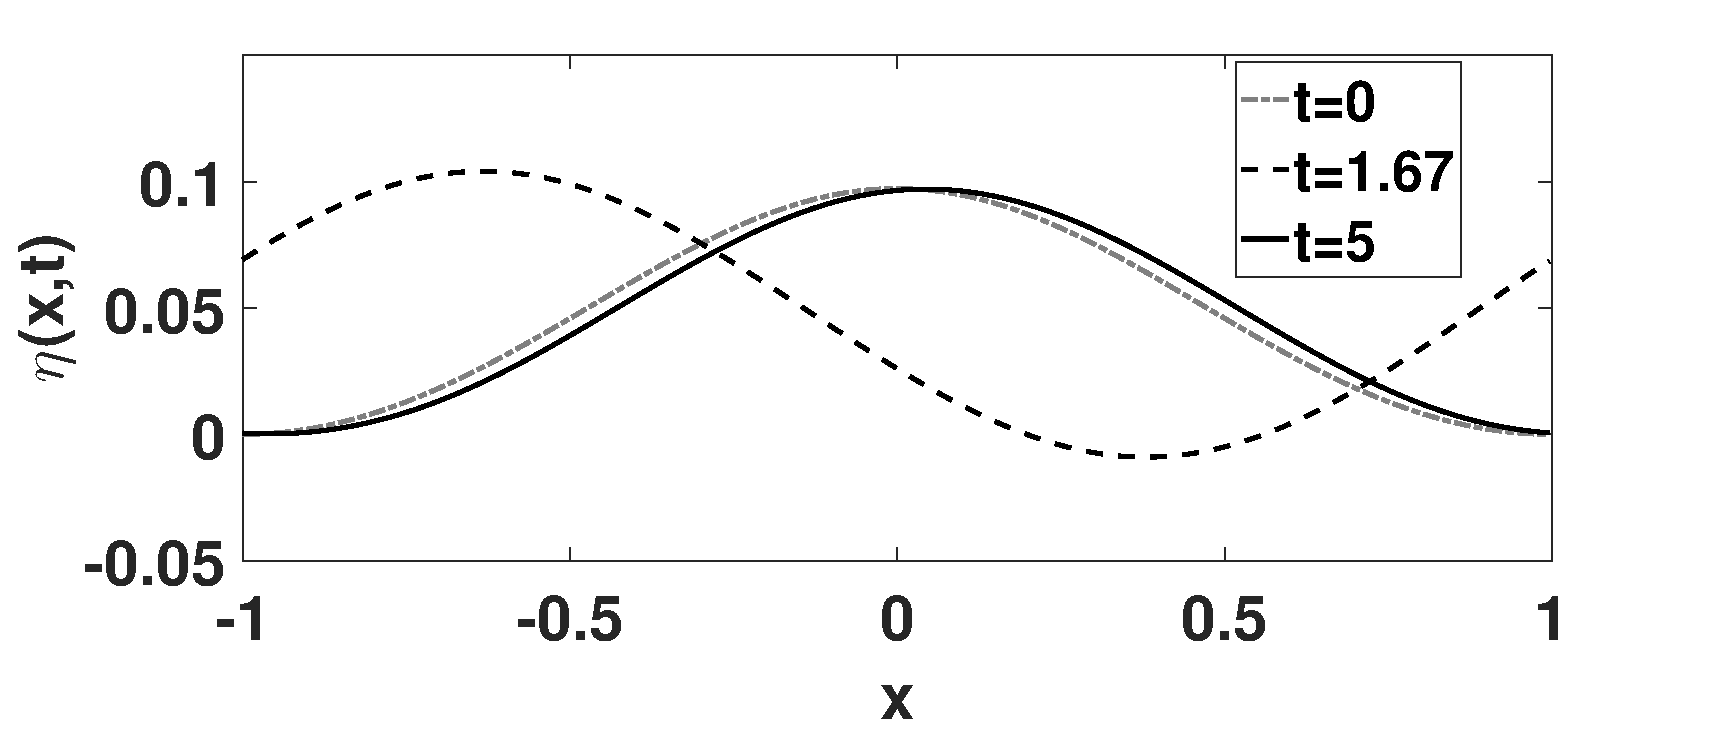
\includegraphics[width=0.48\textwidth]{surf_resp_cnoid_mu_pt2_F_pt02_tf_5NEW} \\
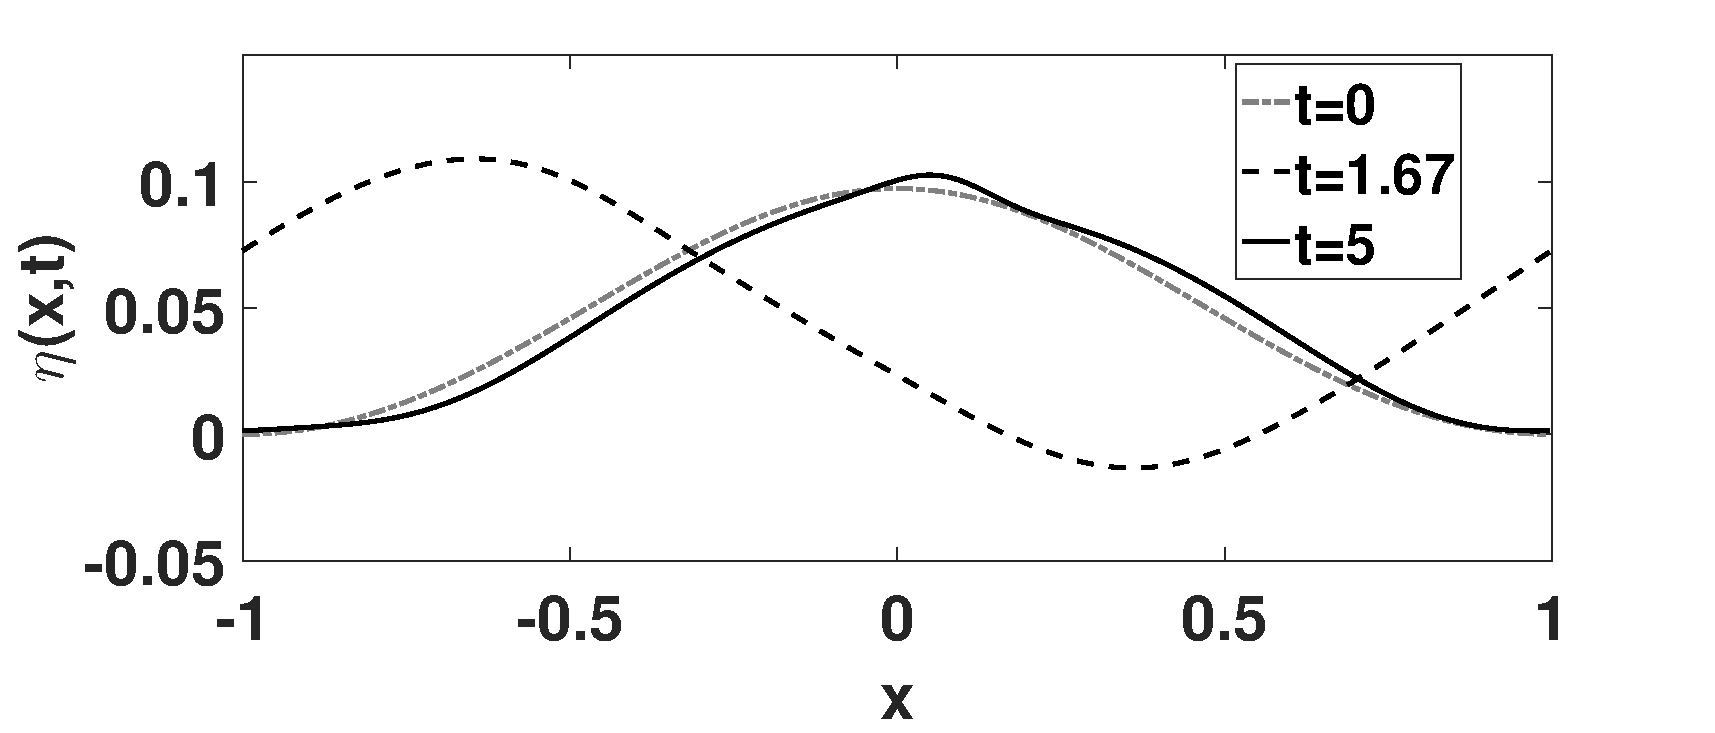
\includegraphics[width=0.48\textwidth]{surf_resp_cnoid_mu_pt2_F_pt2_tf_5NEW}
\end{tabular}
\caption{\small Upper Panel: The surface response $\eta(x,5)$ for a traveling cnoidal solution of the KdV equation with elliptic modulus $\tilde{m}=0.2$ and Froude number $F=0.02$. Lower Panel: The surface response $\eta(x,5)$ for a traveling cnoidal solution of the KdV equation with elliptic modulus $\tilde{m}=0.2$ and Froude number $F=0.2$. The increased Froude number allows for stronger deformation of the surface wave by the rising vortices.}
\label{fig:cnsurfrep}
\end{figure}
%
\begin{figure}[!h]
\centering
\begin{tabular}{cc}
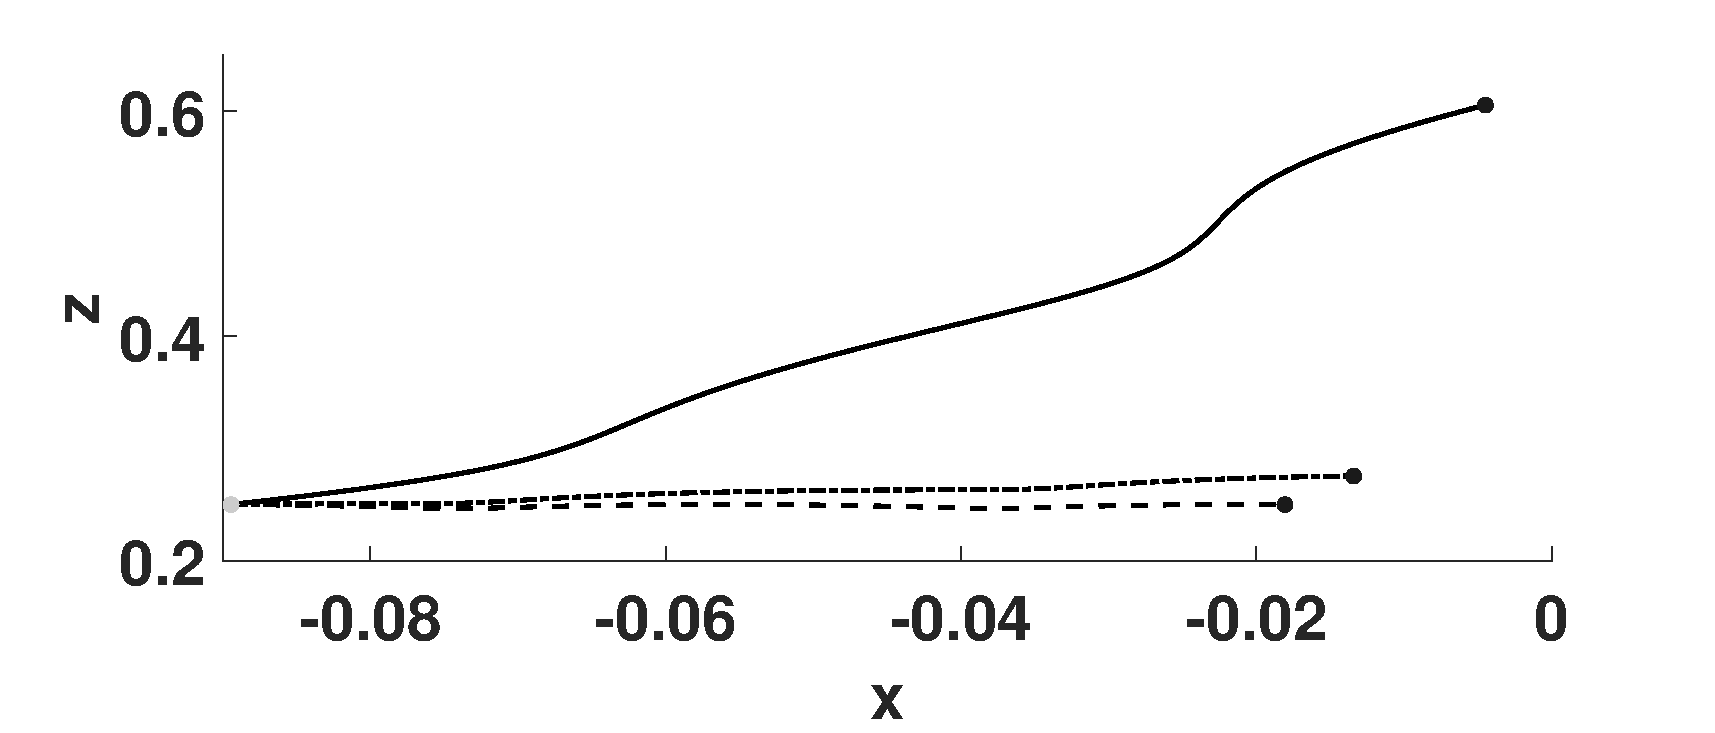
\includegraphics[width=0.48\textwidth]{leftside_cnoid_tracks} & 
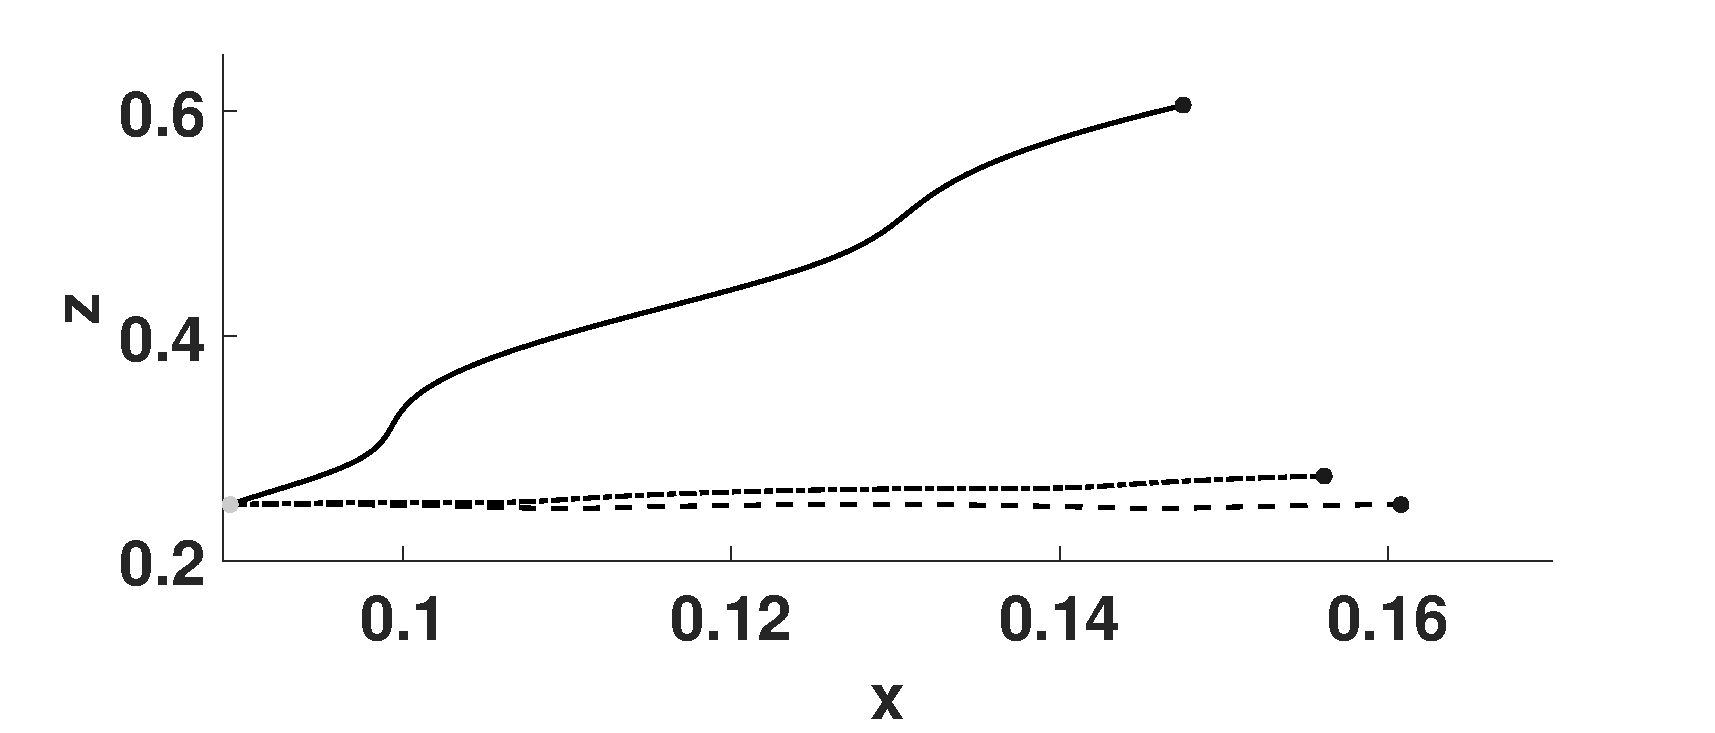
\includegraphics[width=0.48\textwidth]{rightside_cnoid_tracks}
\end{tabular}
\caption{\small Left Panel: Trajectory of the left vortex moving under a cnoidal wave.  Right Panel: Trajectory of the right vortex moving under a cnoidal wave.  In both figures, $0\leq t \leq 5$ for Froude numbers $F=0$ (dashed line), $0.02$ (dashed/dotted line), and $0.2$ (solid line).  The vortex motion starts at the light grey dot and ends at the black dot.}
\label{fig:cntrack}
\end{figure}



Choosing the elliptic modulus to be $\tilde{m}=0.2$, we look at the case of two counter-propagating vortices under the traveling wave where we compare the dynamics for $F=0, 0.02$, and $0.2$.  In all cases, we truncate the DNO expansion at the 32nd term, i.e. $G_{31}$.  We run each simulation up to $t=5=1/\mu$ so that nonlinear effects have time to become asymptotically significant.  Note, we do not consider the case of a breaking wave in this subsection.  We then choose $q_{0}=0$ for ease.        

Setting $F=0$ makes the vortices passive tracers in the bulk of the fluid. As can be seen then from the motion of the vortices in Figure \ref{fig:cntrack}, there is very little difference between the vortex paths for $F=0.02$ and the path of a passive tracer.  Likewise, observing the surface response seen in Figure \ref{fig:cnsurfrep} (Upper Panel), we see the vortex motion has little to no effect on the surface wave profile.  Thus, we can readily argue that the choice of $F=0.02$ corresponds to a sub-critical value of the Froude number.  In contrast, the choice of $F=0.2$ clearly leads to a significant departure of the vortex trajectories from the paths of passive tracers as can be seen in the stronger vortex dynamics in Figure \ref{fig:cntrack}.  Nevertheless, the impact of the vortices on the free surface profile is not very pronounced, see Figure \ref{fig:cnsurfrep} (Lower Panel), since the vortices have not risen near enough to the surface.  However, even if the departure from the passive tracer case is minor as for the $F=0.02$ case, it appears that the presence of vorticity destroys the steady nature of the KdV flow.  However, in special cases with surface tension, it is possible to recover a steady flow in the presence of vorticity \cite{walsh}.  

%\begin{figure}[h]
%\centering
%\begin{tabular}{cc}
%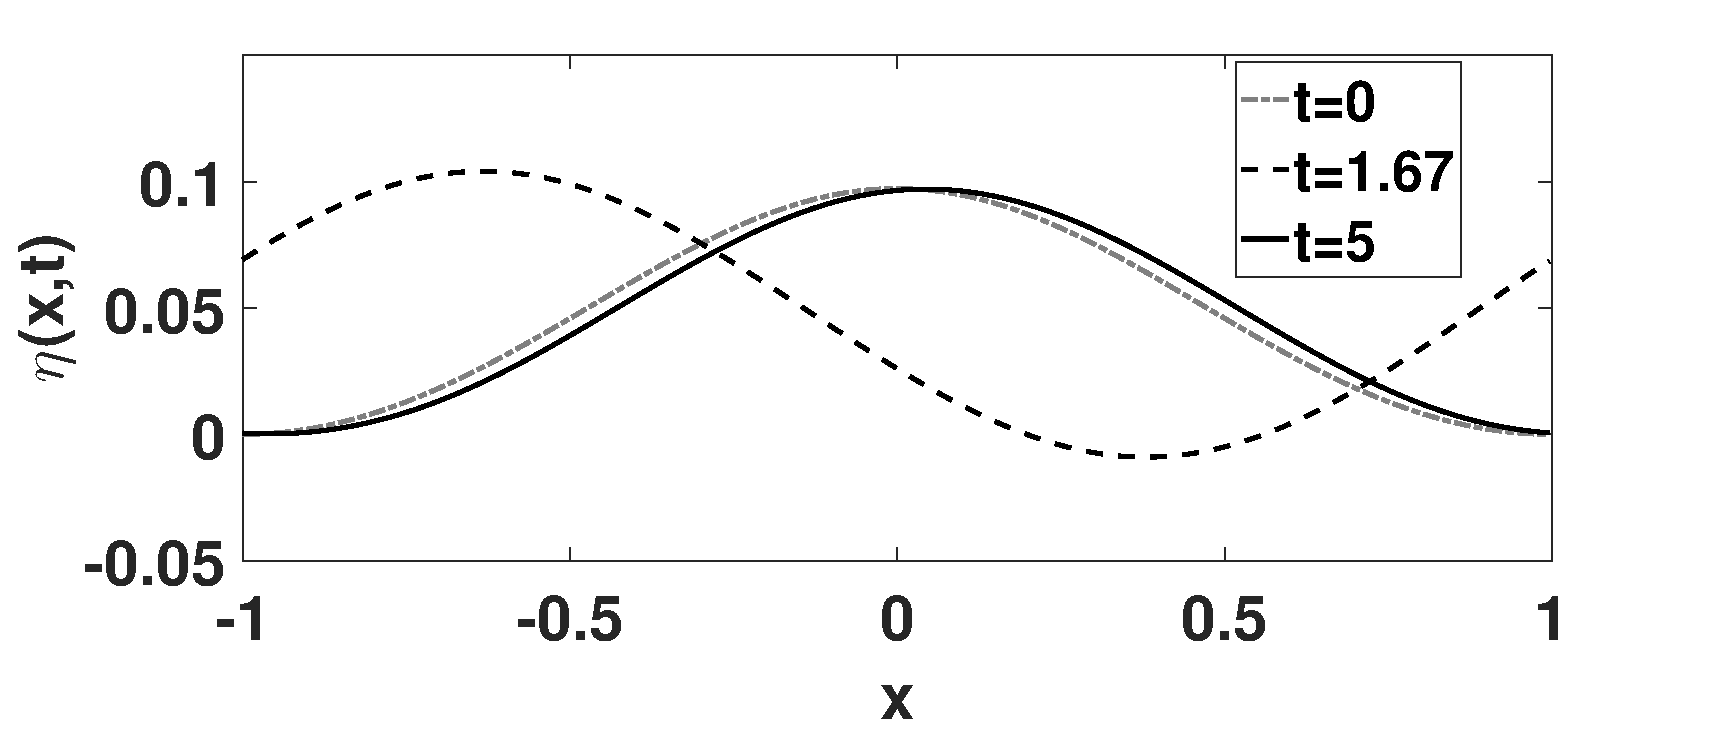
\includegraphics[width=0.48\textwidth]{surf_resp_cnoid_mu_pt2_F_pt02_tf_5NEW} & 
%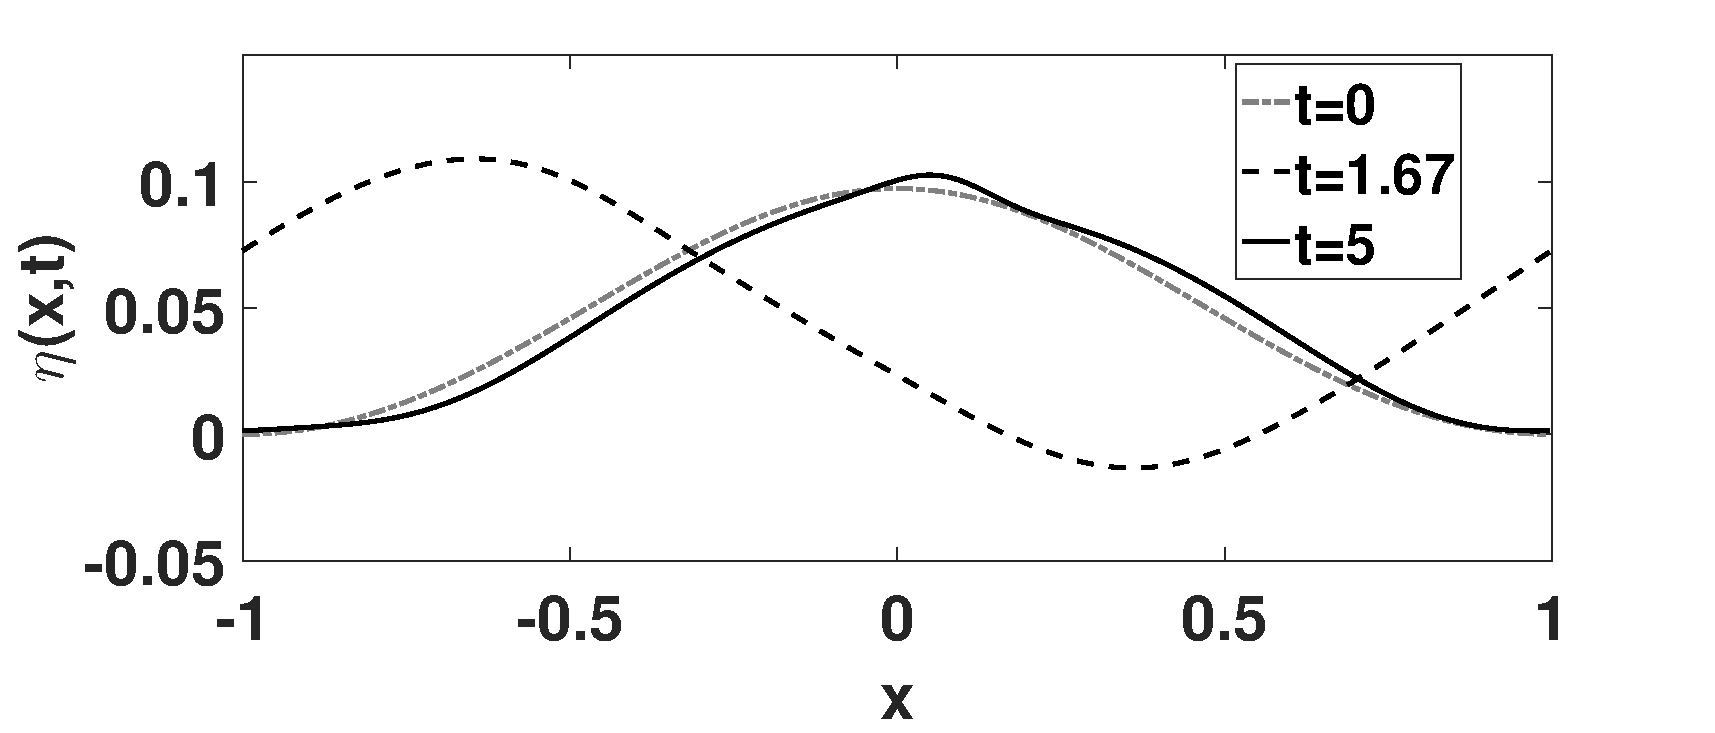
\includegraphics[width=0.48\textwidth]{surf_resp_cnoid_mu_pt2_F_pt2_tf_5NEW}
%\end{tabular}
%\caption{\small Surface response $\eta(x,5)$ for a traveling cnoidal solution of the KdV equation with elliptic modulus $\tilde{m}=0.2$ and Froude number $F=0.02$ (Left Panel) and $F=0.2$ (Right Panel). The increased Froude number allows for stronger deformation of the surface wave by the rising vortices.}
%\label{fig:surfrepcnwk}
%\end{figure}

%\newpage
%%%%%%%%%%%%%%%%%%%%%%%%%%%%%%%%%%%%%%%%%%%%%%%%%%%%%%%%%%%%%%%%%%%%%%%%%%%%%%%%%%
\subsection{Two Counter Propagating Vortices Under an Initially Quiescent Surface}
Throughout the remainder of the paper, we use the initial conditions
\[
\eta(x,0) = 0, ~ Q(x,0) = -\p_{x}\phi_{v}(x,1),
\]
so that the initial surface profile is flat and still.  Likewise, throughout the remainder of the paper, we truncate the DNO expansions at $\tilde{N}=19$; again see Equation \eqref{trunccond} for reference.  On relatively short time scales, we can compare our numerics to the linear theory derived in the previous section.  Using Equation \eqref{surfresp}, we can show that for a pair of counter-rotating vortices, which we describe as the Plus/Minus or PM case, the forcing response for the free surface is given by the function
\begin{equation}
R_{s}(x,t) = 2\sum_{k=1}^{\infty} \frac{\sin(\omega(k)t)}{\omega(k)}\frac{\sinh(\pi \gamma k z_{1})}{\gamma}e^{-\pi \gamma k}\sin(\pi k x_{1})\cos(\pi k x).
\label{twovortsurfresp}
\end{equation}
We note that this result relies on assuming the vortices are essentially stationary.  We expect though that as the vortices rise, there will be a limited time scale over which the linear theory is valid.  To quantify this, we define the time $t_{l}$ which is the first time $t$ at which 
\[
\frac{\gnorm{\eta(\cdot,t)-R_{s}(\cdot,t)}_{2}}{\gnorm{\eta(\cdot,t)}_{2}}\geq \mu
\]    
For $t\geq t_{l}$, we expect nonlinear effects to become significant due to the rise of the vortex pair.    

%
\begin{figure}[!h]
\centering
\begin{tabular}{cc}
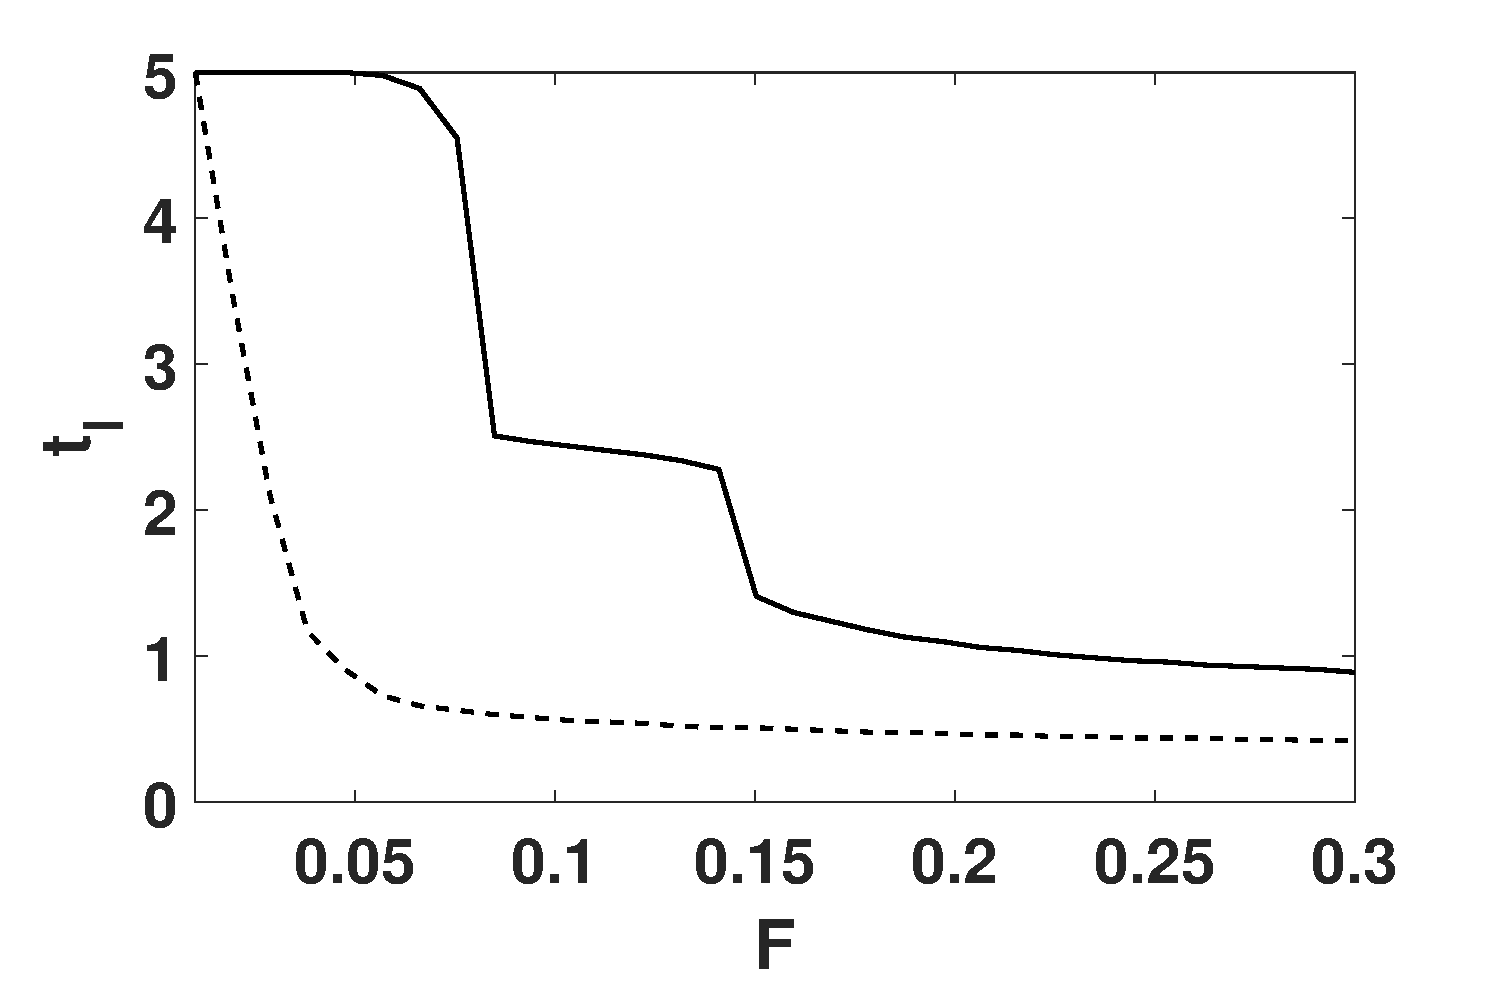
\includegraphics[width=0.46\textwidth]{froude_lin}& 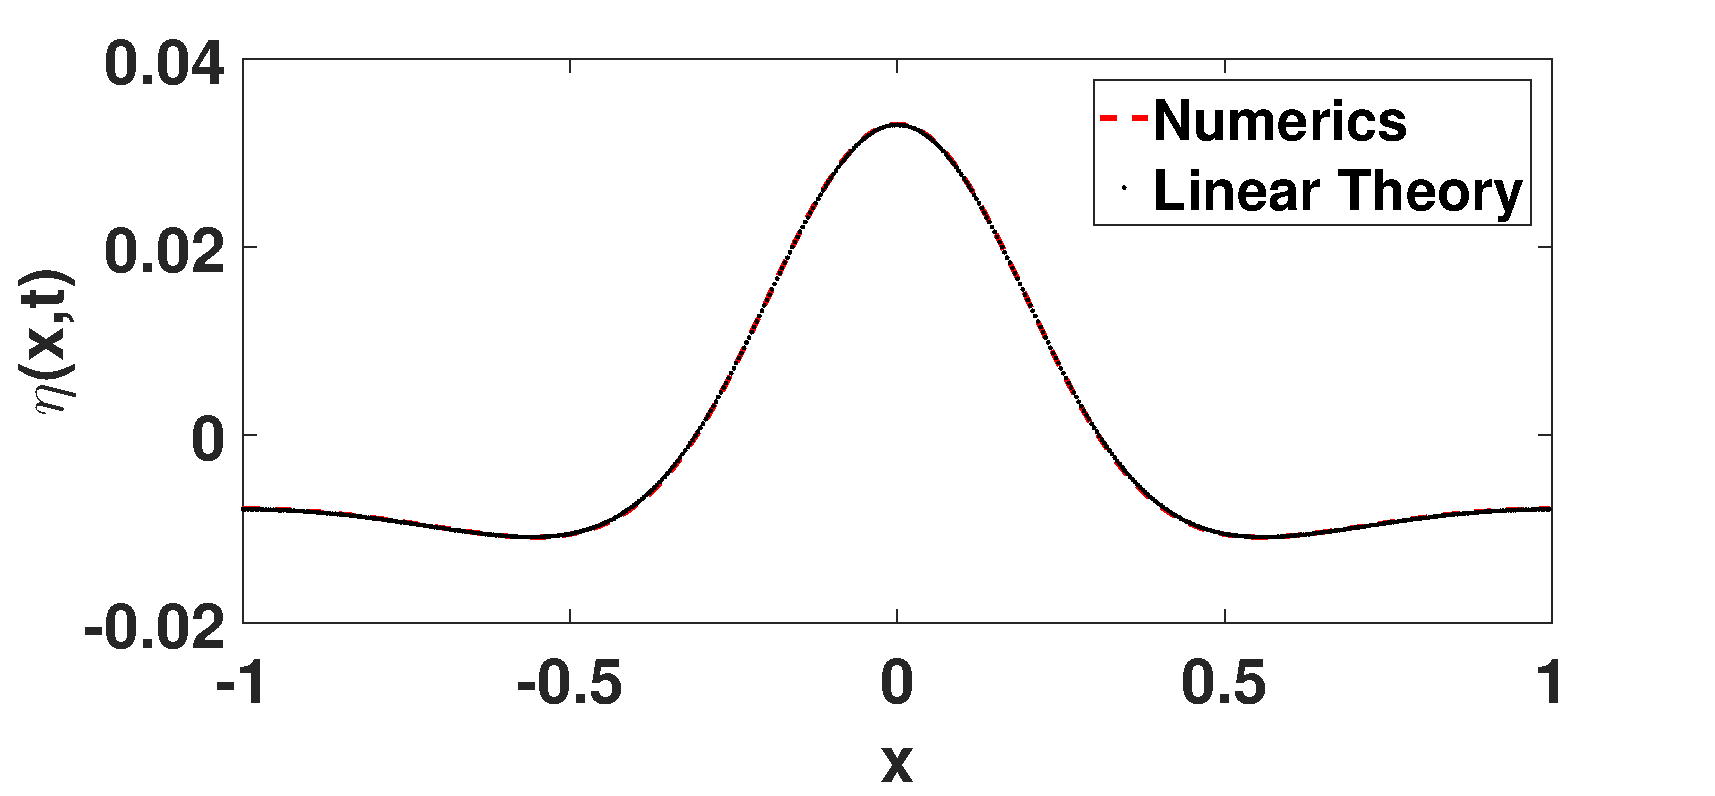
\includegraphics[width=0.5\textwidth]{lin_response_tf_pt5} \\
\end{tabular}
\caption{\small {\bf PM Case}. Left Panel: The quantity $t_{l}$ as a function of $F$  for $\mu=0.1$ (- -) and $\mu=0.2$ (--).  Right Panel: Comparison between linear theory ($\cdot$) and numerics (- -) at $t=0.5$.  For $\mu=0.2$, there are two rapid transitions in the time at which nonlinearity becomes significant around $F=0.15$ in contrast to the one transition for $\mu=0.1$ as seen in the Right Panel.}
\label{fig:linrep}
\end{figure}
In order to study the impact of changing $F$ and $\mu$, we plot $t_{l}$ as a function of $F$ for $0.01\leq F \leq 0.3$ in the cases $\mu=0.1$ and $\mu=0.2$; Figure \ref{fig:linrep}, (Left Panel).  This figure displays several fascinating qualities.  We first notice that $t_{l}$ is markedly shorter for $\mu=0.1$ than for $\mu=0.2$.  Given our choice of initial vortex positions though, see Equation \eqref{initxpostv}, the smaller $\mu$ value has the vortices start closer together, so that they must rise faster for the same value of $F$, thus explaining the discrepancy.  Related to this, we also see the response of $t_{l}$ to changes in $F$ is fundamentally different for the different choices of $\mu$.  The most conspicuous differences are the rapid transitions in $t_{l}$.  In the $\mu=0.2$ case, for $F$ near $.1$ and $.15$, the value of $t_{l}$ undergoes two sharp transitions.  However, for $\mu=0.1$, the increased speed of the rising vortices only allows for one transition region for $F$ near $.05$.  While it is tempting then to describe at least one of these transitions as a transition from the sub to super critical vortex regime, this would be an arbitrary decision, and not appropriate over the different parameter choices.  What appears to be true instead is that in contrast to previous literature, the behavior of vortices in the shallow water regime is strongly parameter dependent, and ready dichotomies of behavior are not as apparent.  

In the particular case for $F=0.2$ and $\mu=0.2$ at $t=0.5$, we see in Figure \ref{fig:linrep} (Right Panel) that the linear response is quite accurate.  The falling troughs, or scars, seen in much of the existing literature \cite{marcus,tryggvason} are present.  However, we note that in previous work, the formation of mounds in the surface profile corresponded to the vortices being near the wave crest.  Thus, the presence of the bottom boundary and the concomitant upwelling it induces causes wave profiles to form at far shorter time scales and for different reasons than reported in the previous literature.  

To further explore the role of nonlinearity then, we now look at how the breaking time $t_{b}$ and breaking distance $\delta_{b}$ depend on the choice of $F$ and $\mu$.  As seen in Figure \ref{fig:froudecomp} (Left Panel), the breaking time is markedly shorter for $\mu=0.1$ than $\mu=0.2$, which is in accord with our choice of initial vortex positions and in line with the results above for $t_{l}$.  We emphasize though that in all cases $t_{b}>t_{l}$, and so we are always outside the linear regime at the breaking time for both $\mu=0.1$ and $\mu=0.2$.  We also see that the vortices are able to get closer to the surface for $\mu=0.1$ than for $\mu=0.2$ as seen by comparing $\delta_{b}$ in the right panel of Figure \ref{fig:froudecomp}.  Finally, it is worth emphasizing that for the range of Froude numbers examined, $.1\leq F \leq .3$, no readily identifiable critical behavior emerges.  Thus, trying to use either $t_{b}$ or $\delta_{b}$ to define sub or super critical regimes seems inappropriate.  
%
\begin{figure}[!h]
\centering
\begin{tabular}{cc}
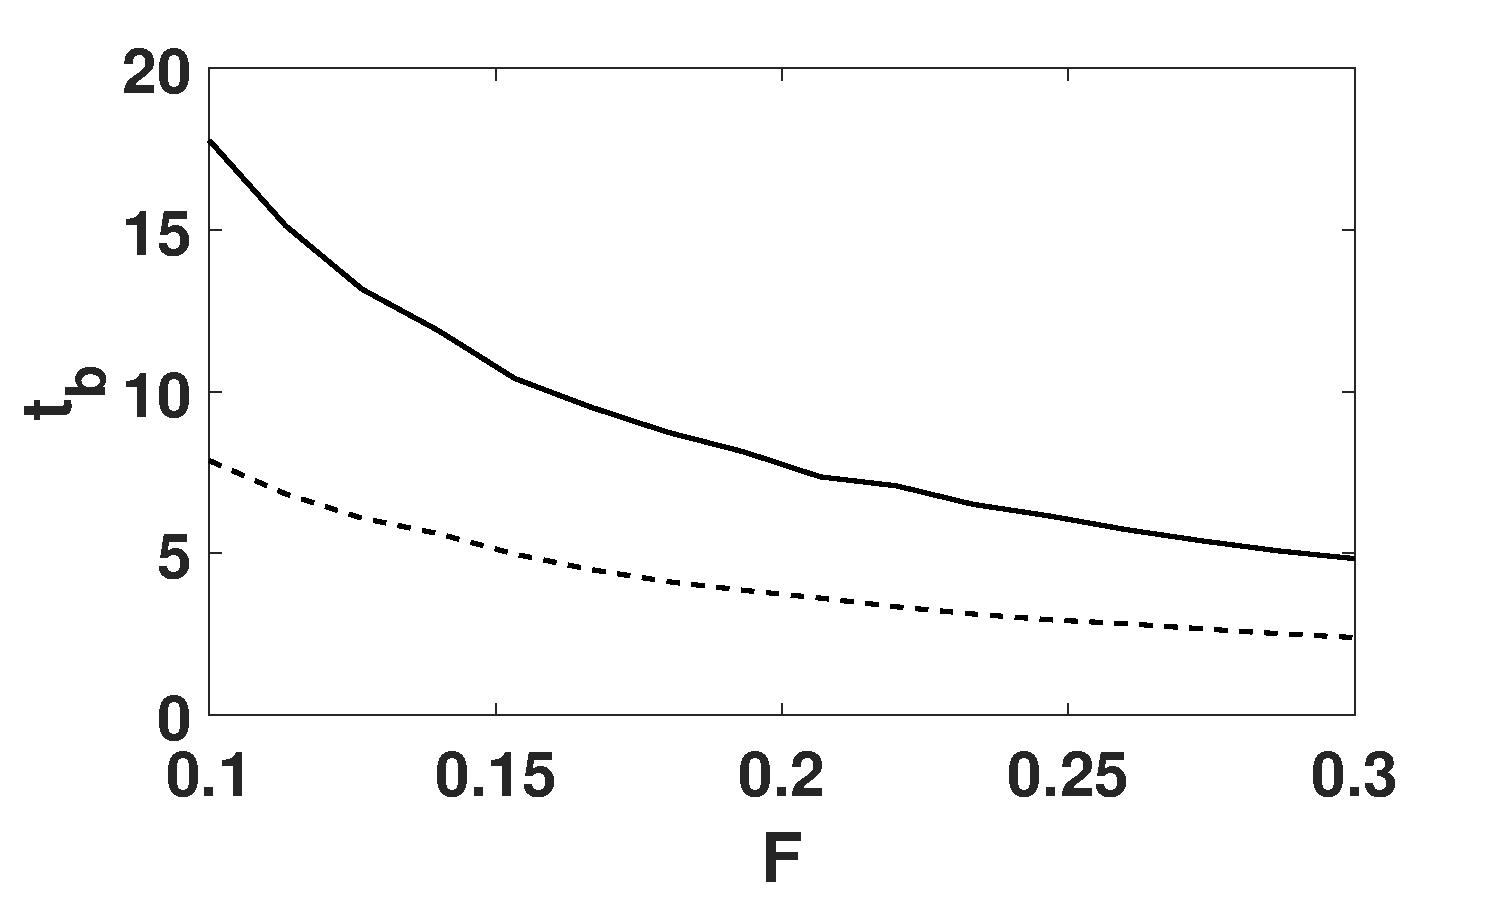
\includegraphics[width=0.5\textwidth]{froude_comp_pm} &
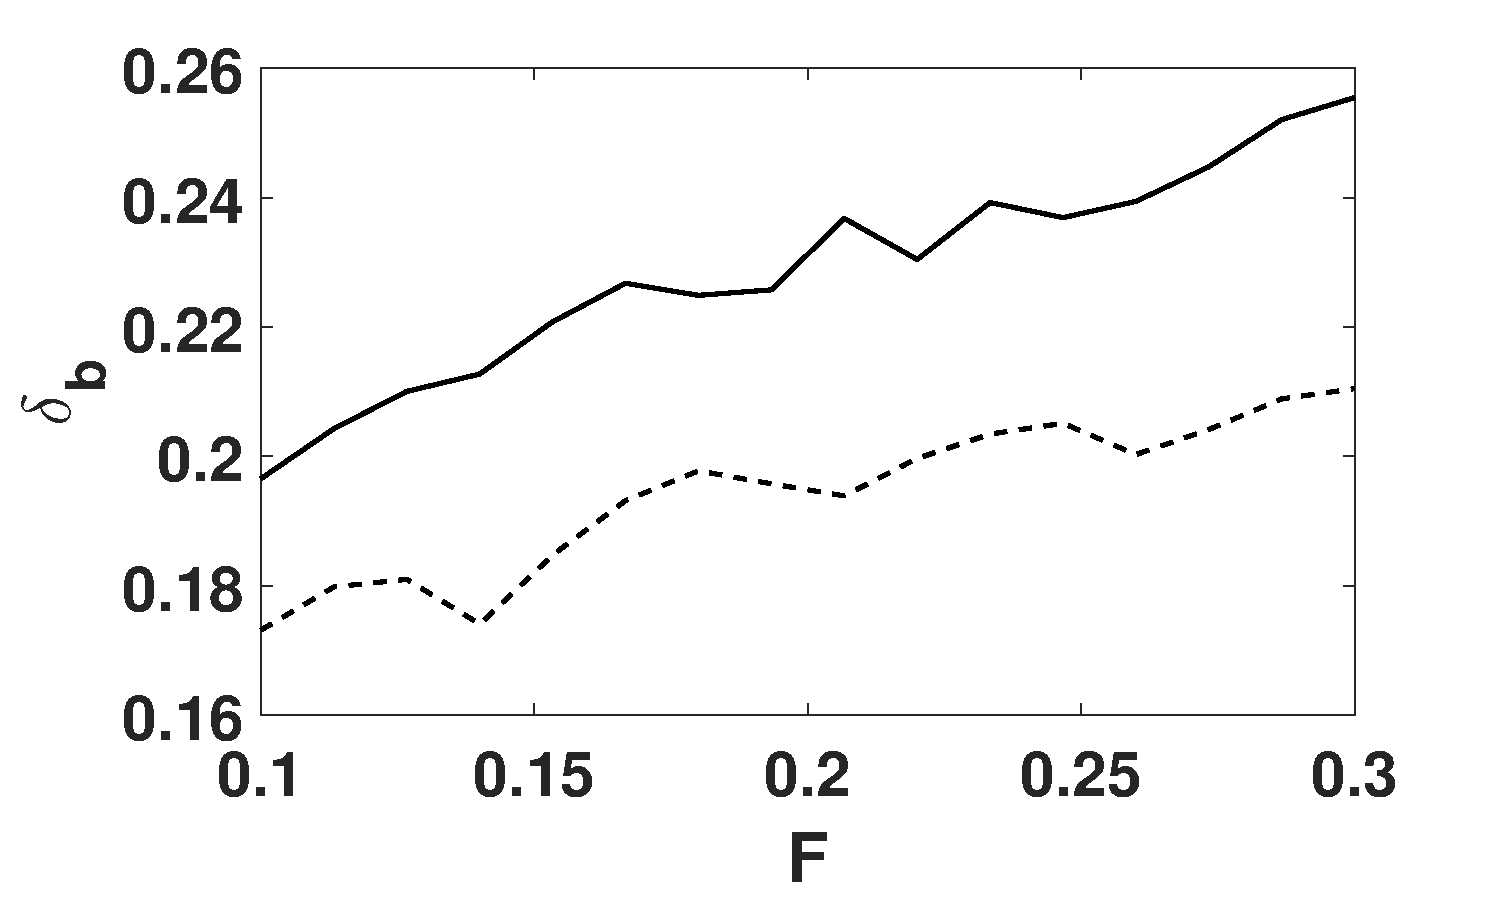
\includegraphics[width=0.5\textwidth]{zmb_pm}
\end{tabular}
\caption{\small {\bf PM Case}. Left Panel: Plot of the breaking time $t_{b}$ as a function of Froude number $F$. Right Panel: Plot of the breaking distance $\delta_{b}$ as a function of Froude number $F$.  In both panels, we look at $\mu=0.1$ (- -) and $\mu=0.2$ (--). The smaller parameter value $\mu=0.1$ allows for a faster rise of the vortices (Left Panel) and a closer approach to the surface (Right Panel).}
\label{fig:froudecomp}
\end{figure}

To build greater intuition, we now choose the particular values $F=0.2$ and $\mu=0.2$ and look at simulations of the surface, vortex positions, and energy for $0\leq t \leq t_{b}\approx 9$.  As seen in Figure \ref{fig:surfrepFpt2}, comparing the surface profiles at $t=3$, $6$, and $9$, higher frequency phenomena and distinguished peaks form as the vortices rise.  We also see that the vortices behave as though they are deflected by a solid boundary once they are close enough to the free surface; see Figure \ref{fig:surfrepFpt2} (Right Panel).  This figure also shows that our method reproduces the dynamics of a vortex pair in qualitative agreement with \cite{tryggvason}, even though this is a rough comparison since the results in \cite{tryggvason} are for infinite depth.  As seen in Figure \ref{fig:eprof_tv}, the amount of energy shared between the surface and the vortices stays relatively constant up to about $t=4$.  But once the vortices come into close proximity of the free surface, they begin pumping kinetic energy $K(t)$ at a greater rate as seen if Figure \ref{fig:eprof_tv} at $t=9\approx t_{b}$. In contrast, the potential energy $P(t)$ remains relatively constant even up to $t=9\approx t_{b}$.  
%
\begin{figure}[!h]
\centering
\begin{tabular}{cc}
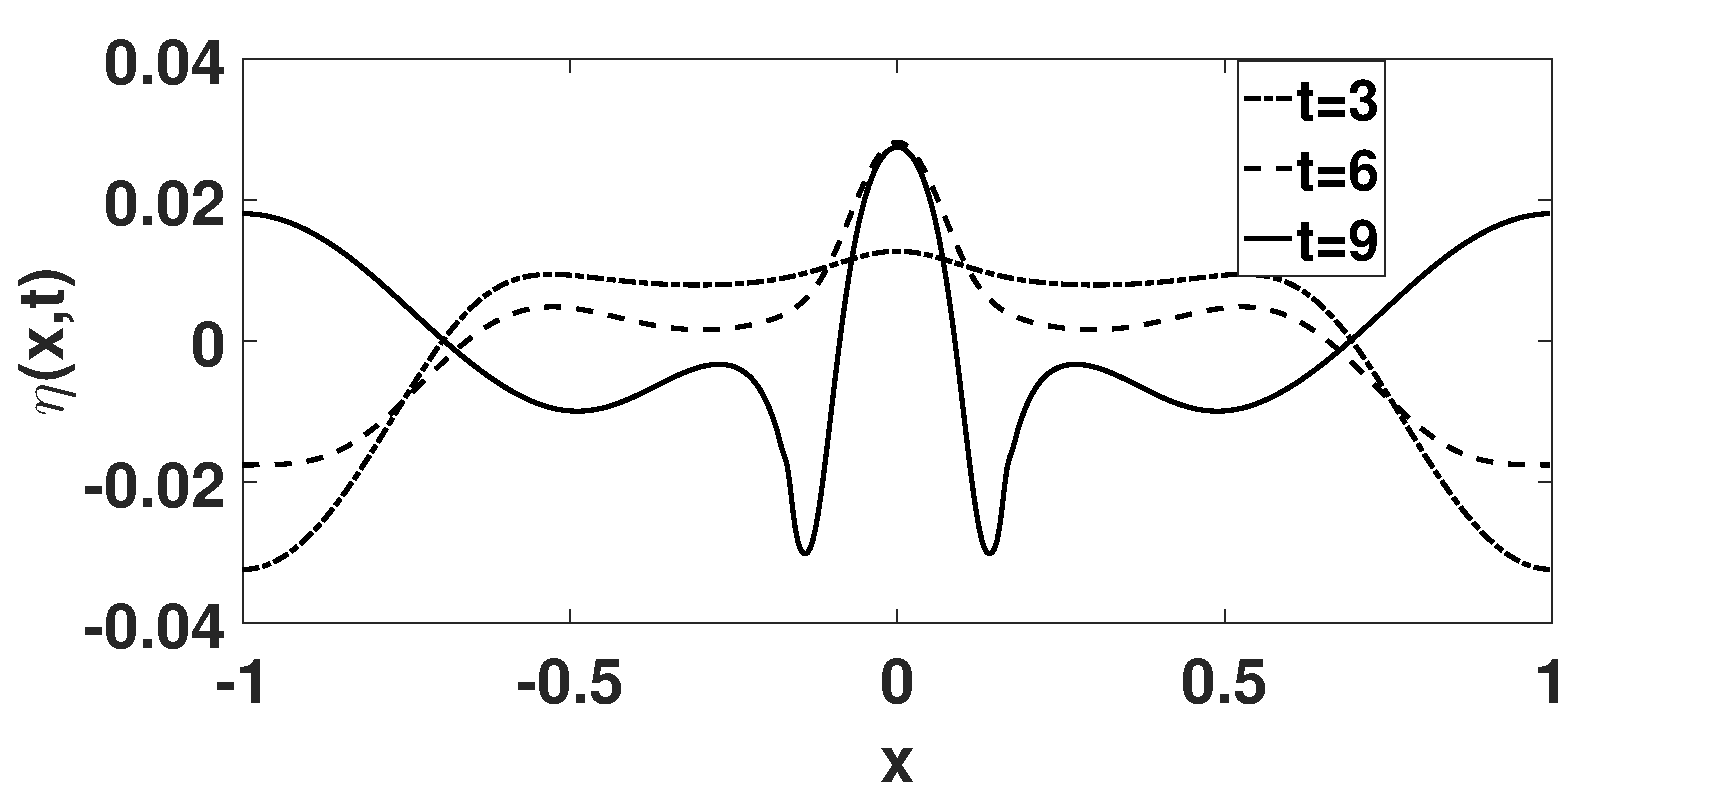
\includegraphics[width=0.5\textwidth]{surf_resp_mu_pt2_F_pt2} \\
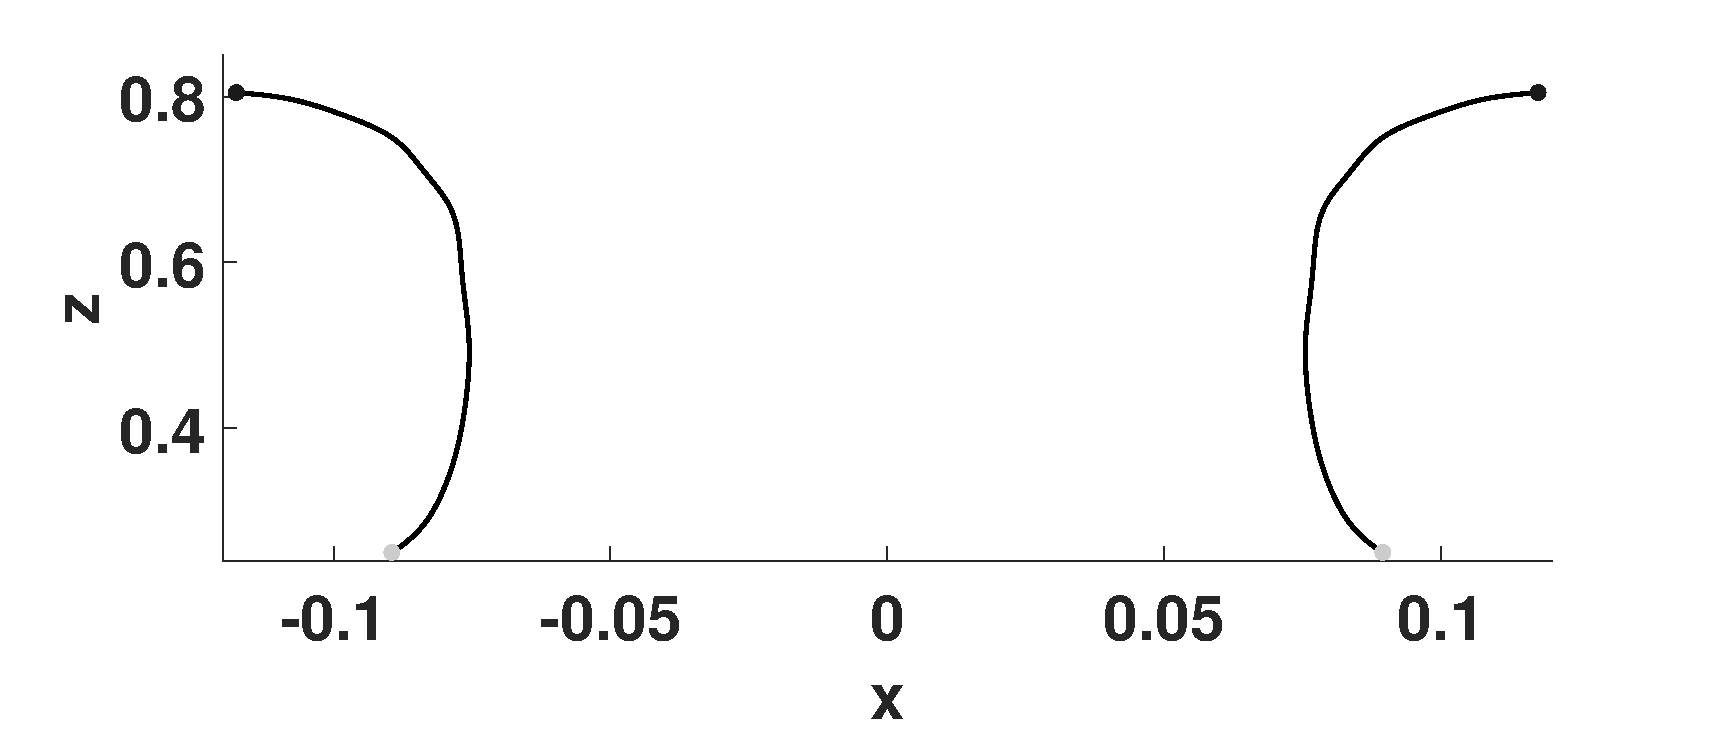
\includegraphics[width=0.5\textwidth]{tracks_F_pt2_tf_9}
\end{tabular}
\caption{\small {\bf PM Case}. Left Panel: Surface response $\eta(x,t)$ over two vortices.  Right Panel: Motion of the two counter-propagating vortices for $0\leq t \leq 9$.  The light grey dots indicate where the vortices begin and the black dots indicate their positions at $t=9$.  $F=0.2$ and $\mu=0.2$ in both panels.}
\label{fig:surfrepFpt2}
\end{figure}
%
\begin{figure}[!h]
\centering
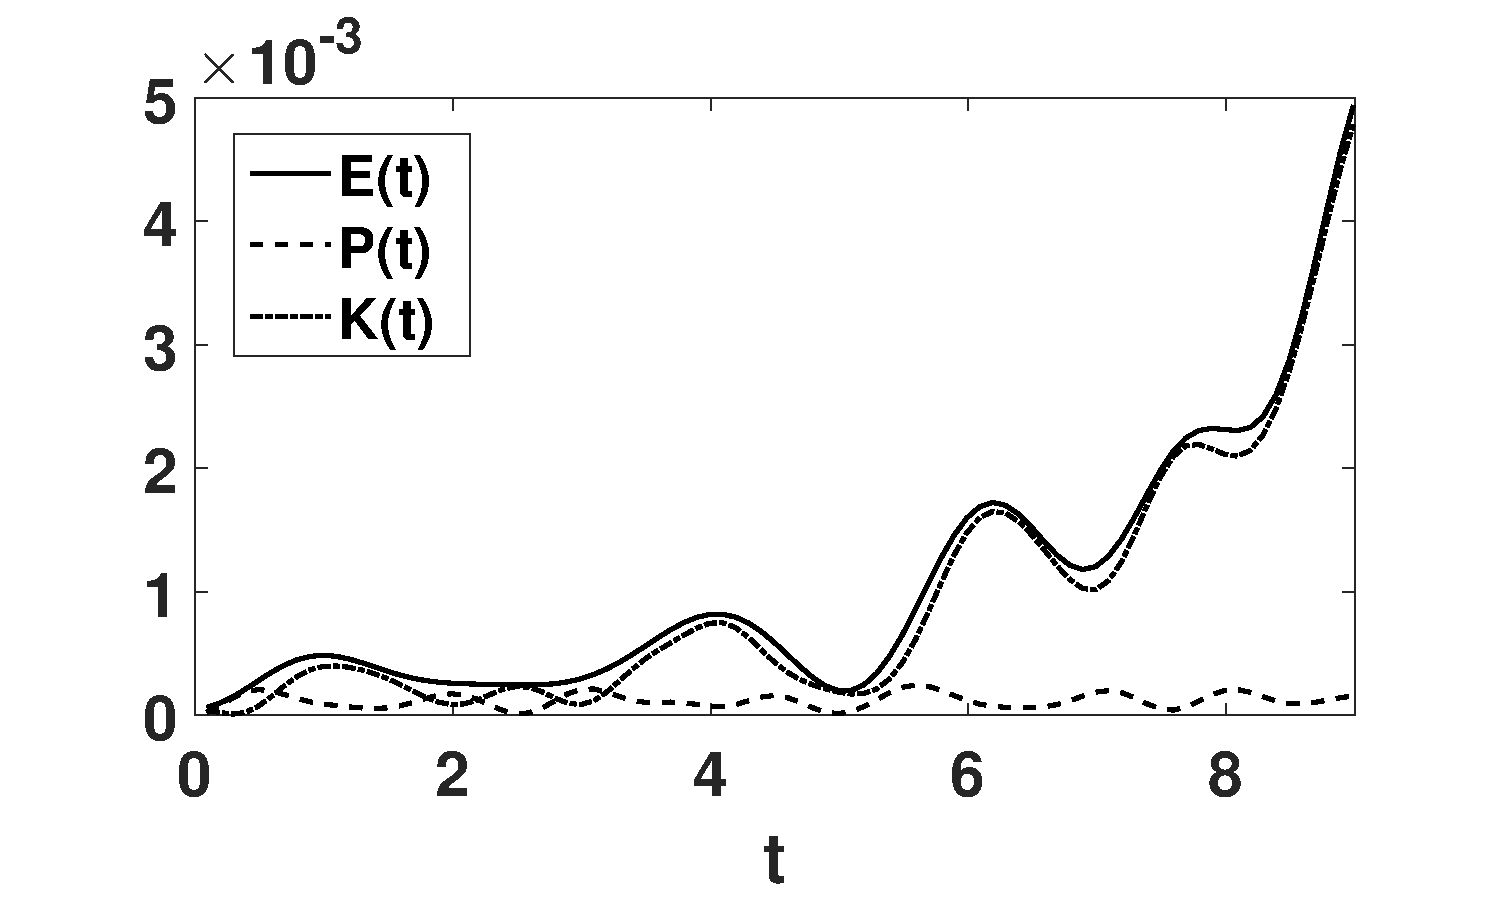
\includegraphics[width=0.6\textwidth]{energy_profile_mu_pt2_F_pt2_tv}
\caption{\small {\bf PM Case}. Surface energy $E(t)$, potential energy $P(t)$, and kinetic energy, $K(t)$, profiles for a surface over two vortices for $0\leq t \leq 9$ for $F=0.2$ and $\mu=0.2$.}
\label{fig:eprof_tv}
\end{figure}

%%%%%%%%%%%%%%%%%%%%%%%%%%%%%%%%%%%%%%%%
\subsection{Four Vortices: Plus/Plus, Minus/Minus}
Using the same numerical scheme and parameters as from above, we now look at the case of four vortices, chosen with vortex strengths
\[
\Gamma_{1}=\Gamma_{2}=1, ~ \Gamma_{3}=\Gamma_{4}=-1.
\]
We refer to this choice of vortex strengths as the `Plus/Plus, Minus/Minus' (PPMM) case.  We study this for both the clustered (CPPMM) and equispaced (EPPMM) initial vortex configurations.  

As seen by comparing Figure \ref{fig:froudecomp_ppmm}, Left and Right Panels, it is still the case that the smaller $\mu$ value corresponds to a shorter breaking time.  Further, we see that the breaking time is almost double that in the CPPMM case compared to the EPPMM case, so the difference in initial vortex placement has a significant impact.  This is even more striking when we look at the difference initial vortex configurations have on $\delta_{b}$.  In the EPPMM case, $\delta_{b}$ is still clearly separated by $\mu$ value over the entire range of $F$.  In contrast to the PM case above though, $\delta_{b}$ now exhibits small fluctuations around a mean value as $F$ changes; see Figure \ref{fig:froudecomp_ppmm}, Lower Right Panel.  In even further contrast to the PM case above, in the CPPMM case, the uppermost vortices rise to nearly equal heights for both $\mu=0.1$ and $\mu=0.2$ across a range of Froude numbers; see Figure \ref{fig:froudecomp_ppmm}, Lower Left Panel.  We also note that $\delta_{b}$ is markedly larger in the CPPMM case than in the EPPMM case, showing the vortices do not get as close the surface before breaking occurs in the CPPMM case. 
%
\begin{figure}[!h]
\centering
\begin{tabular}{cc}
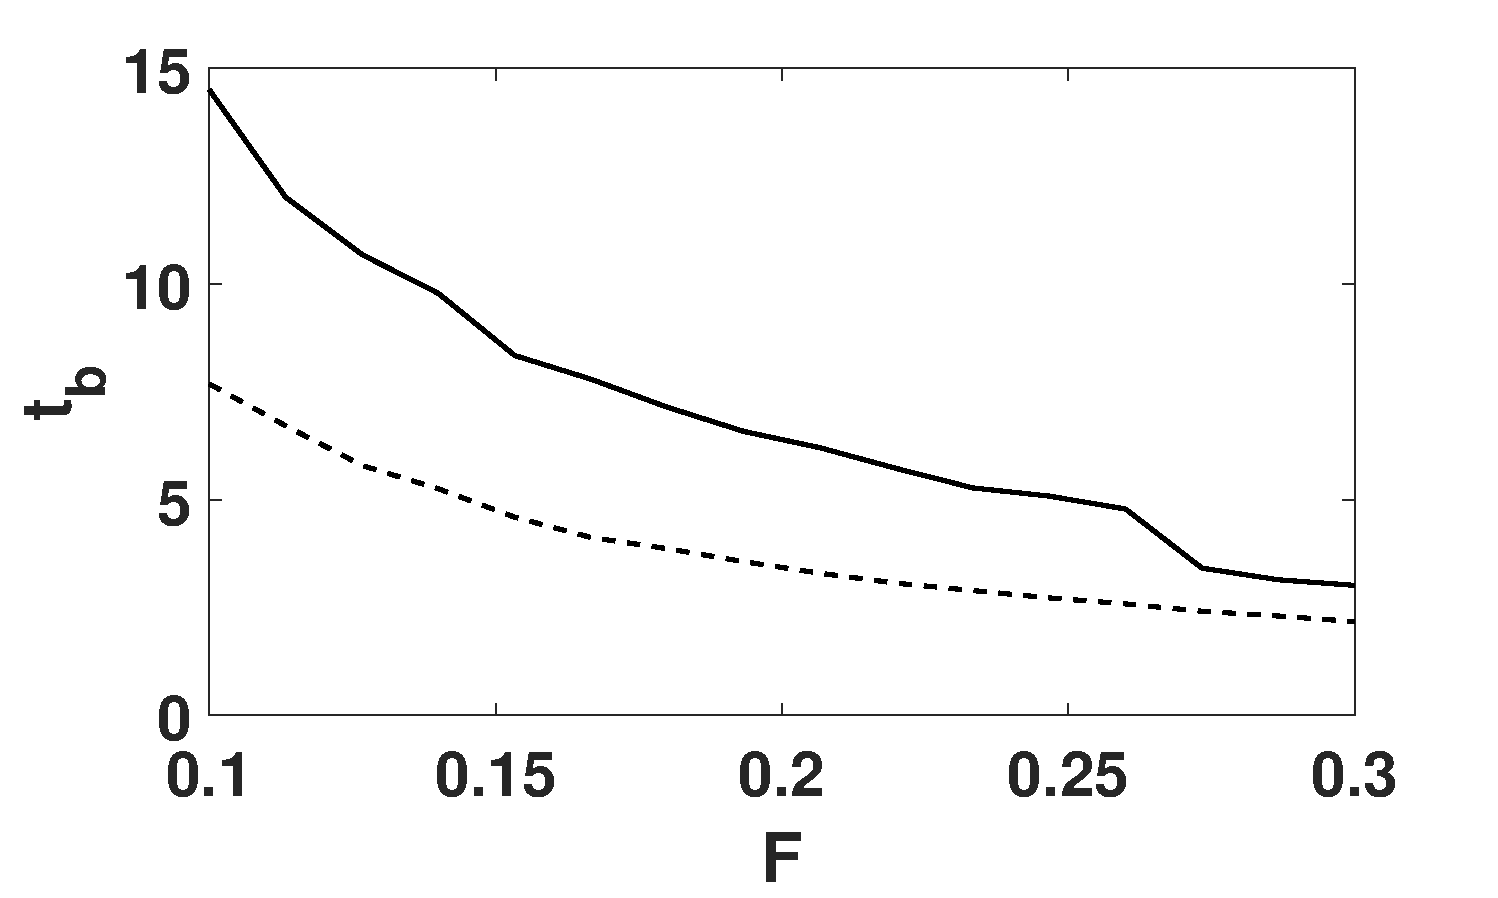
\includegraphics[width=0.5\textwidth]{froude_comp_ppmm} & 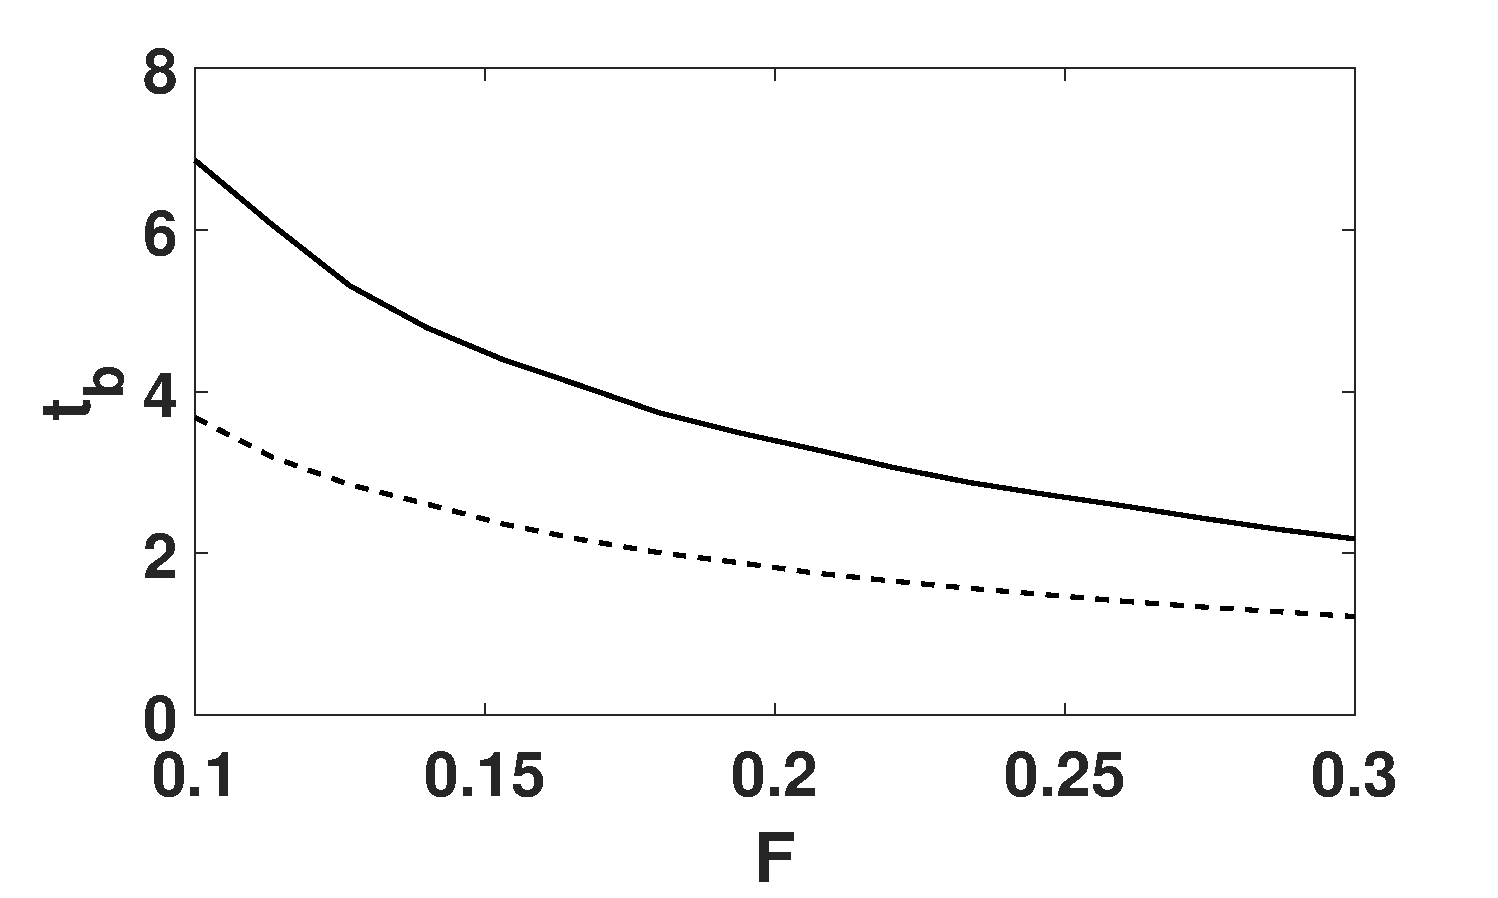
\includegraphics[width=0.5\textwidth]{froude_comp_ppmm_sym}\\
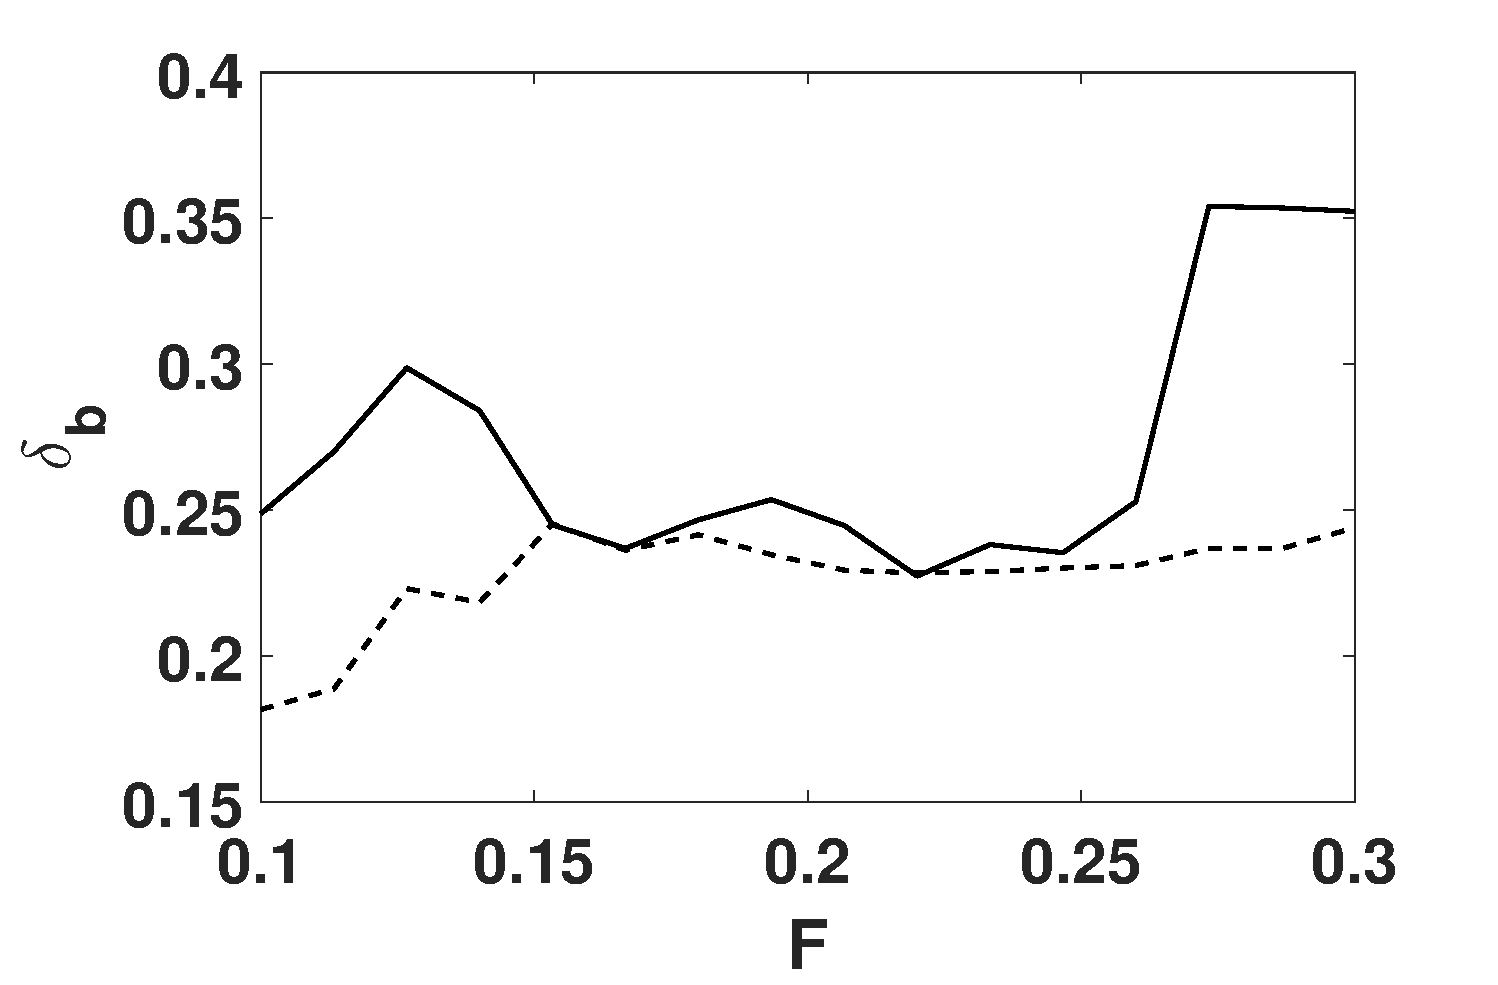
\includegraphics[width=0.5\textwidth]{zmb_ppmm} & 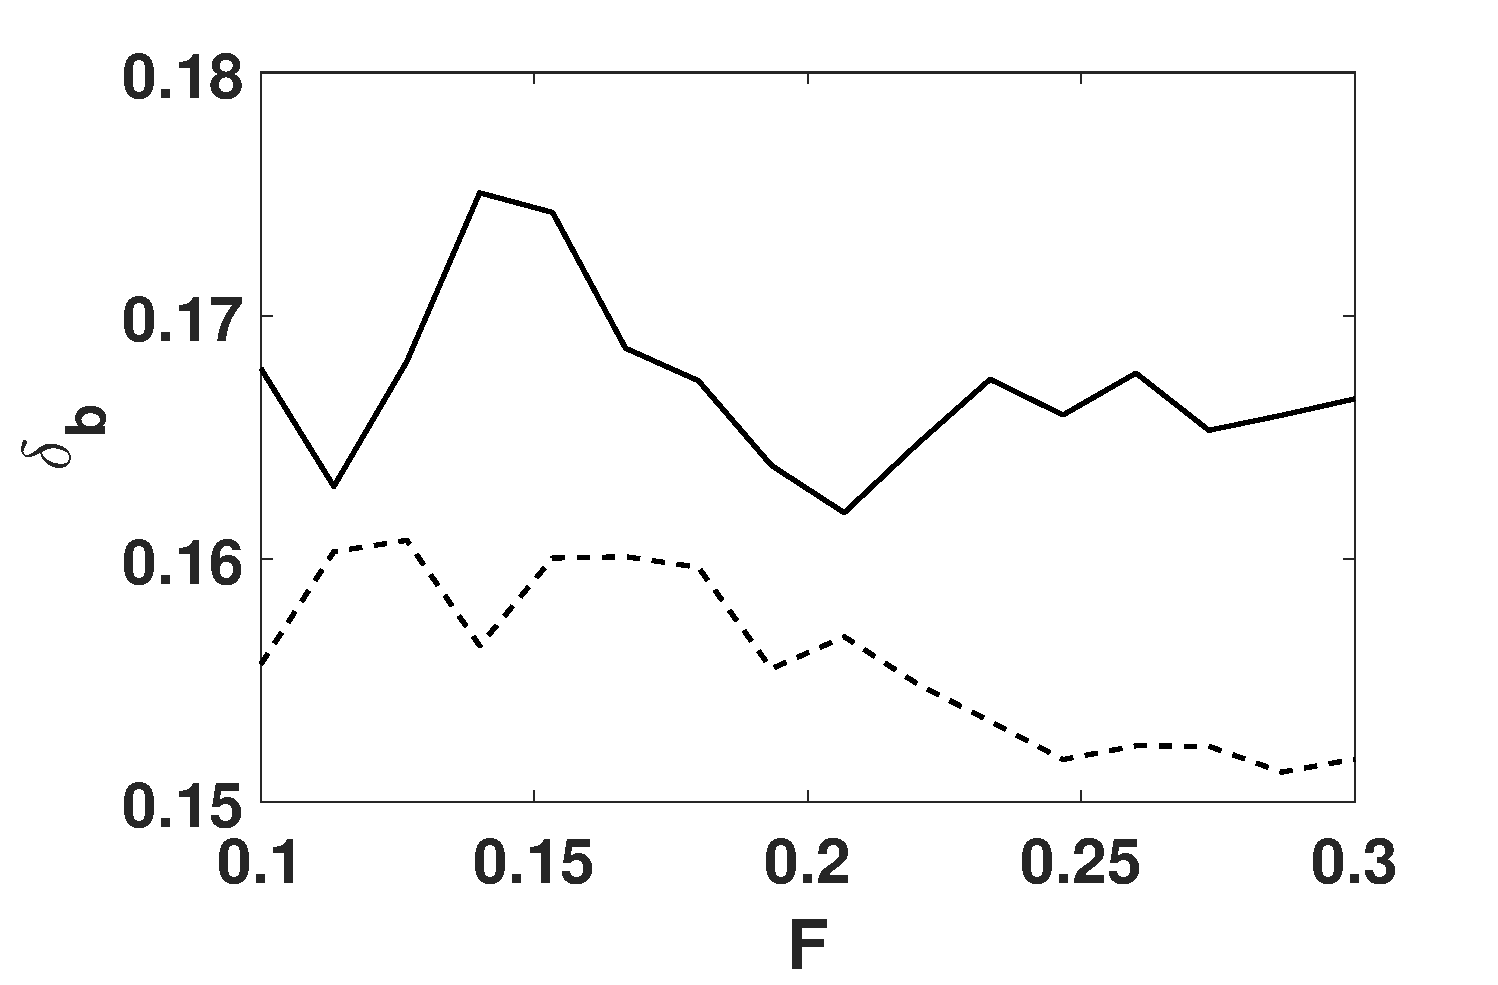
\includegraphics[width=0.5\textwidth]{zmb_ppmm_sym}
\end{tabular}
\caption{\small {\bf PPMM Case}. Upper Panels: Plots of the breaking times $t_{b}$ as a function of Froude number $F$ for $\mu=0.1$ (- -) and $\mu=0.2$ (--).  Lower Panels: Plots of the breaking distances $\delta_{b}$ as a function of Froude number $F$ for $\mu=0.1$ (- -) and $\mu=0.2$ (--). Left Panels: Plots of the breaking time and distance for four vortices starting in the CPPMM configuration.  Right Panels: Plots of the breaking time and distance for four vortices starting in the EPPMM configuration.  The CPPMM case allows for longer breaking times but the EPPMM case allows for closer approach of the vortices to the surface.}
\label{fig:froudecomp_ppmm}
\end{figure}

To better understand this added complexity stemming from the presence of a greater number of vortices, we now examine in detail the dynamics of the surface, vortices, and energy in both the CPPMM and EPPMM cases for $F=0.2$ and $\mu=0.2$ running each case up to the respective values of $t_{b}$.  As seen in Figure \ref{fig:surfrepppmm}, while the time scales are drastically shorter in the EPPMM case than the CPPMM case, the nature of the surface profiles are not markedly different.  Where significant changes emerge is in the behavior of the vortex paths as seen in Figure \ref{fig:tracksppmm}.  In the CPPMM case (Left Panel), the vortices undergo more circular motion, thus explaining the longer onset of breaking in the CPPMM case.  This is also reflected in the rate at which energy enters the surface; see Figure \ref{fig:eprof_ppmm} (Left Panel).   Also of interest is the observed correlation between complexity of vortex dynamics and the exchange of potential and kinetic energy; compare Figures \ref{fig:eprof_ppmm} and \ref{fig:surfrepppmm} (Left Panels) to (Right Panels).  As can be seen, the added circular motion of the vortices in the CPPMM case causes oscillations back and forth between $P(t)$ and $K(t)$.
%
\begin{figure}[!h]
\centering
\begin{tabular}{cc}
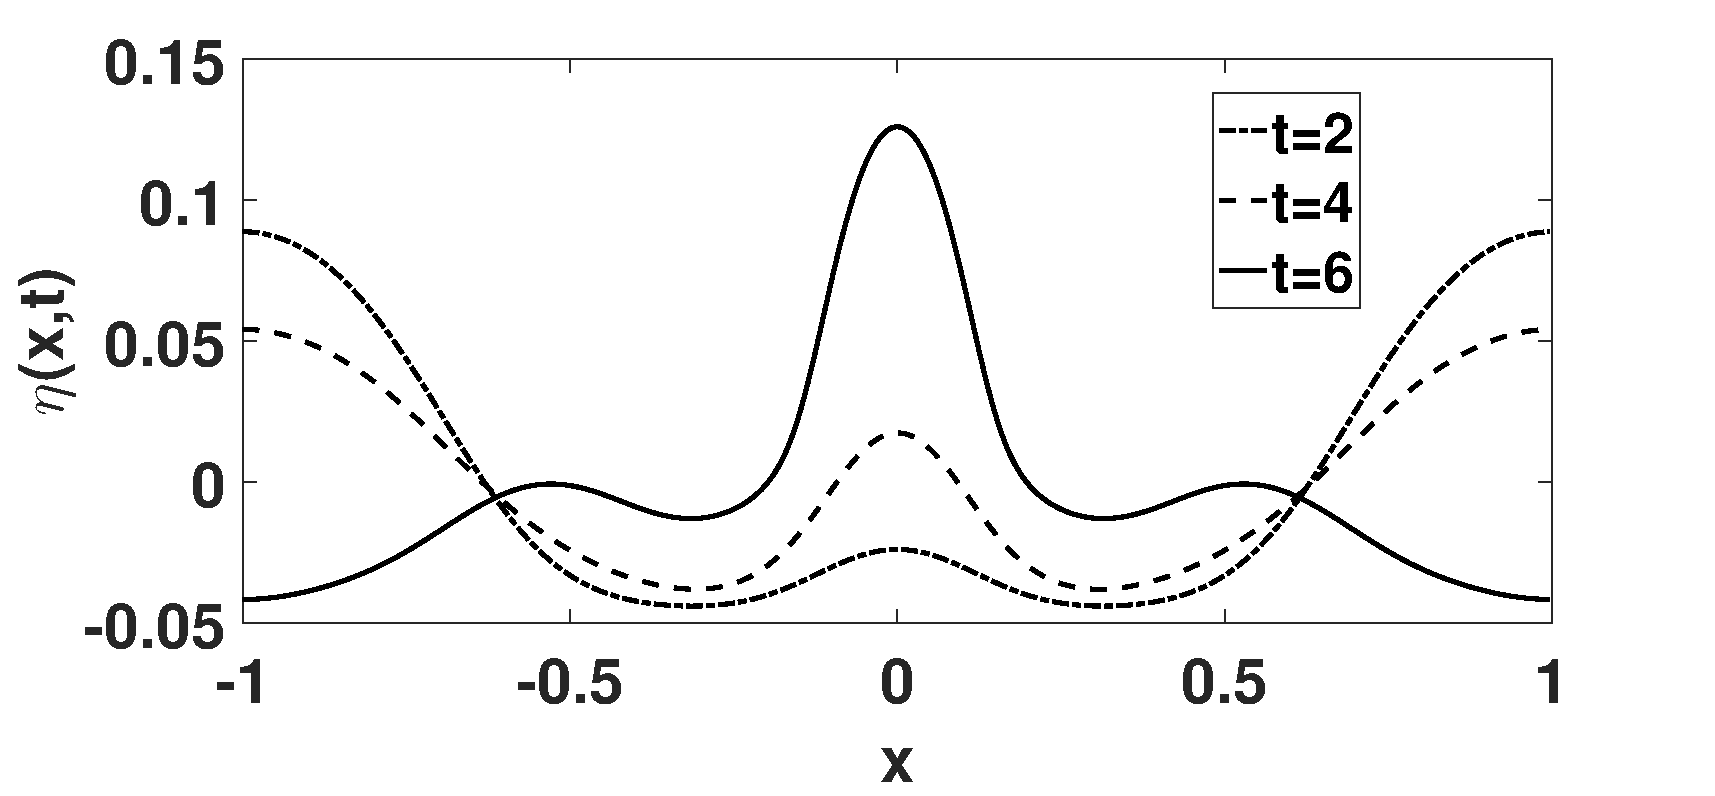
\includegraphics[width=0.5\textwidth]{surf_resp_mu_pt2_F_pt2_ppmm} & 
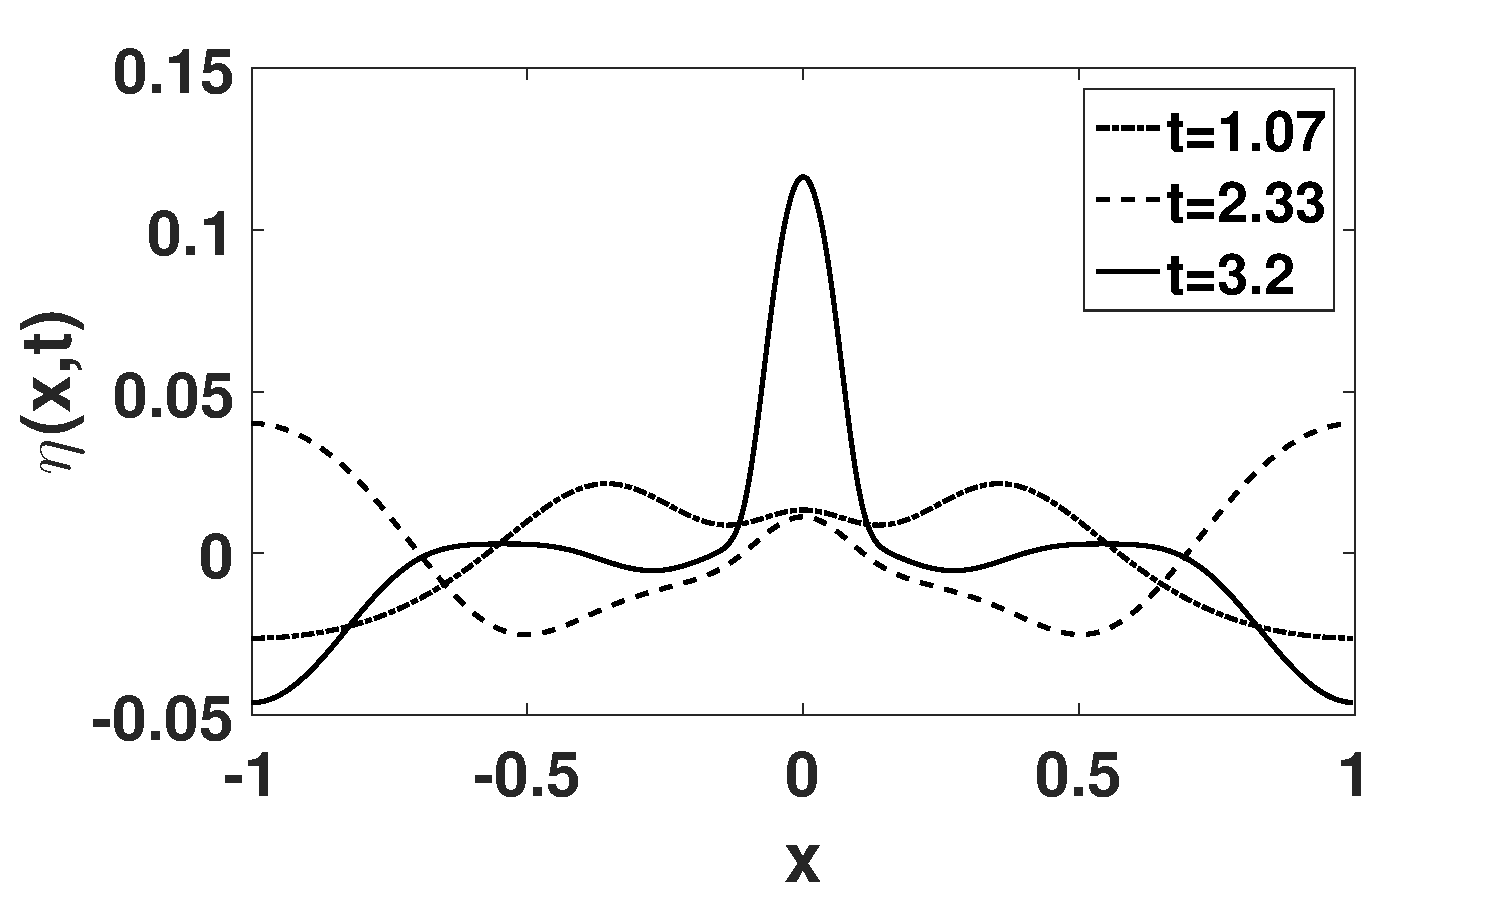
\includegraphics[width=0.5\textwidth]{surf_resp_mu_pt2_F_pt2_ppmm_sym}
\end{tabular}
\caption{\small {\bf PPMM Case}. Left Panel: Surface response $\eta(x,t)$ over four vortices in the CPPMM configuration. Right Panel: Surface response $\eta(x,t)$ over four vortices in the EPPMM configuration.  $F=0.2$ and $\mu=0.2$ in both panels.}
\label{fig:surfrepppmm}
\end{figure}
%
\begin{figure}[!h]
\centering
\begin{tabular}{cc}
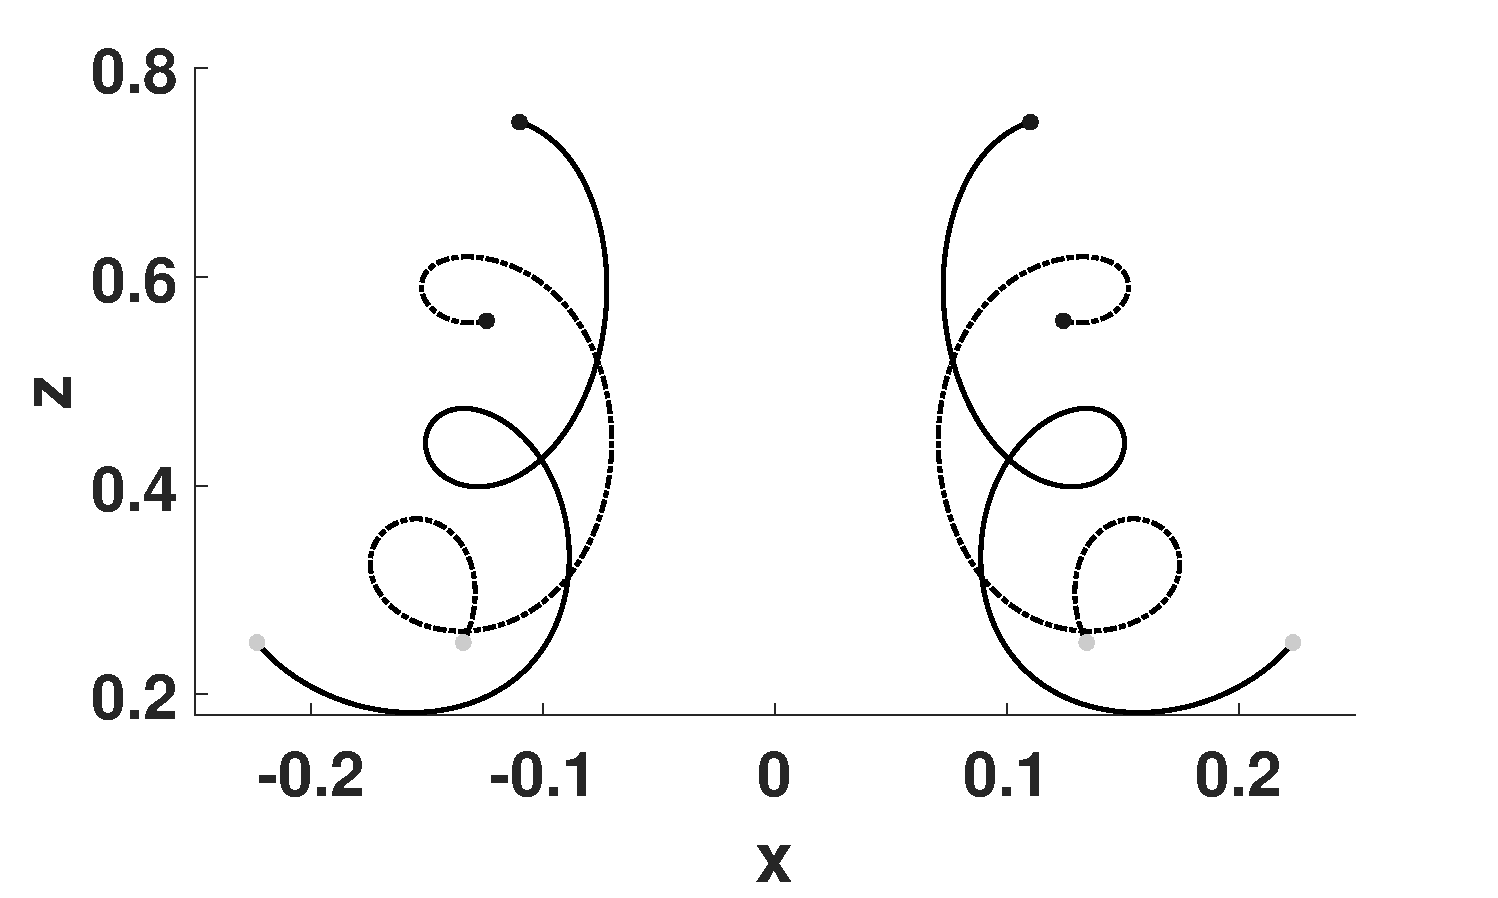
\includegraphics[width=0.5\textwidth]{tracks_F_pt2_tf_6_ppmm} & 
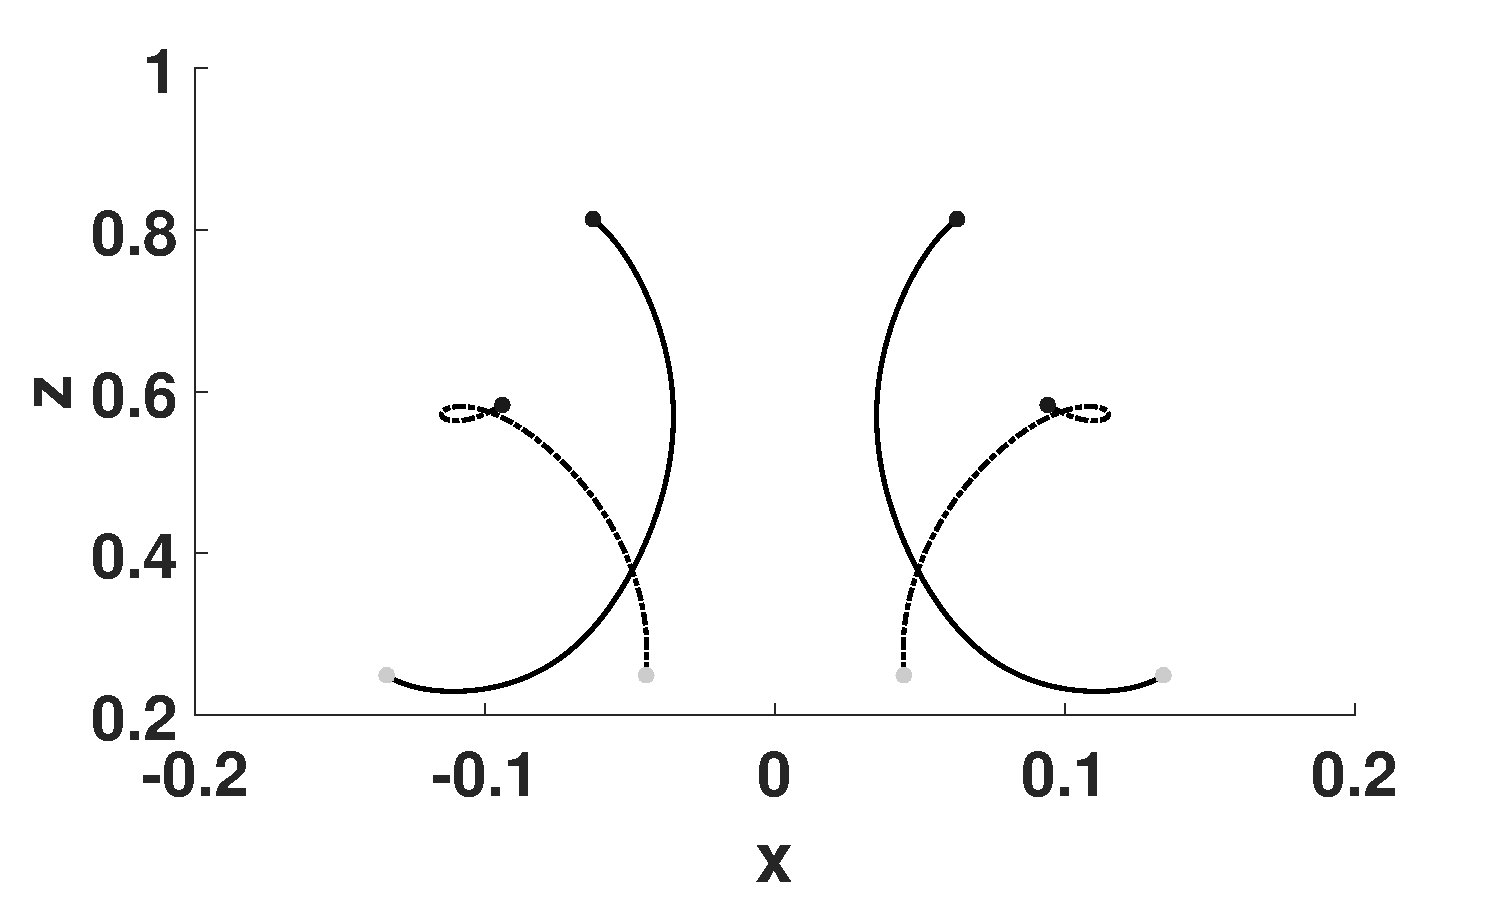
\includegraphics[width=0.5\textwidth]{tracks_F_pt2_tf_3pt2_ppmm_sym}
\end{tabular}
\caption{\small {\bf PPMM Case}. Left Panel: Vortex paths for four vortices in the CPPMM configuration. Right Panel: Vortex paths for four vortices in the EPPMM configuration. $F=0.2$ and $\mu=0.2$ in both panels, and simulations are run for $0\leq t \leq t_{b}$.}
\label{fig:tracksppmm}
\end{figure}
%
\begin{figure}[!h]
\centering
\begin{tabular}{cc}
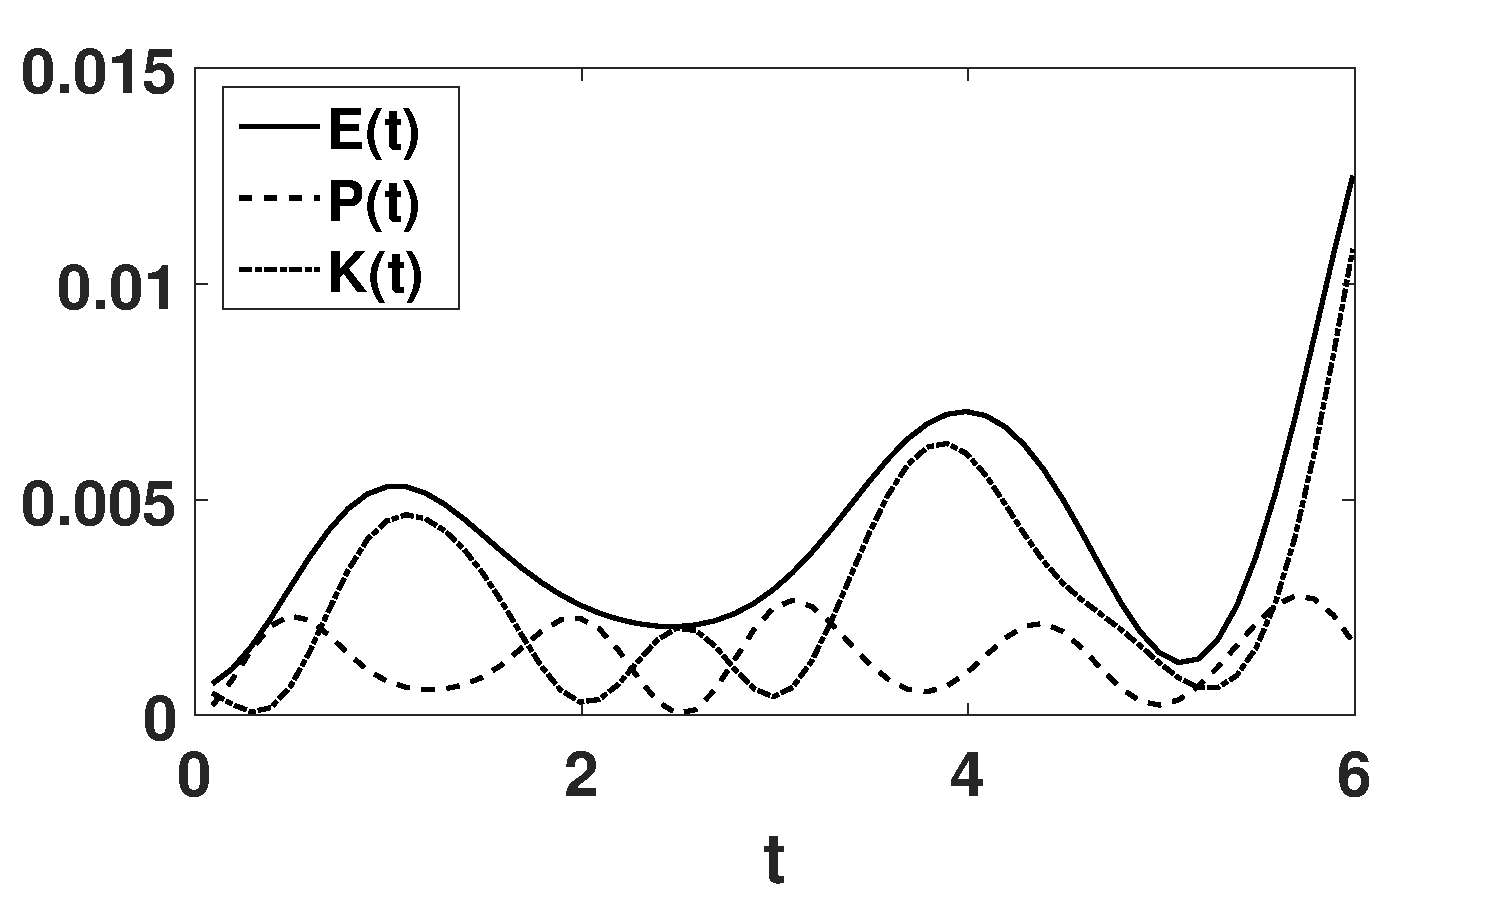
\includegraphics[width=0.5\textwidth]{energy_profile_mu_pt2_F_pt2_ppmm} &
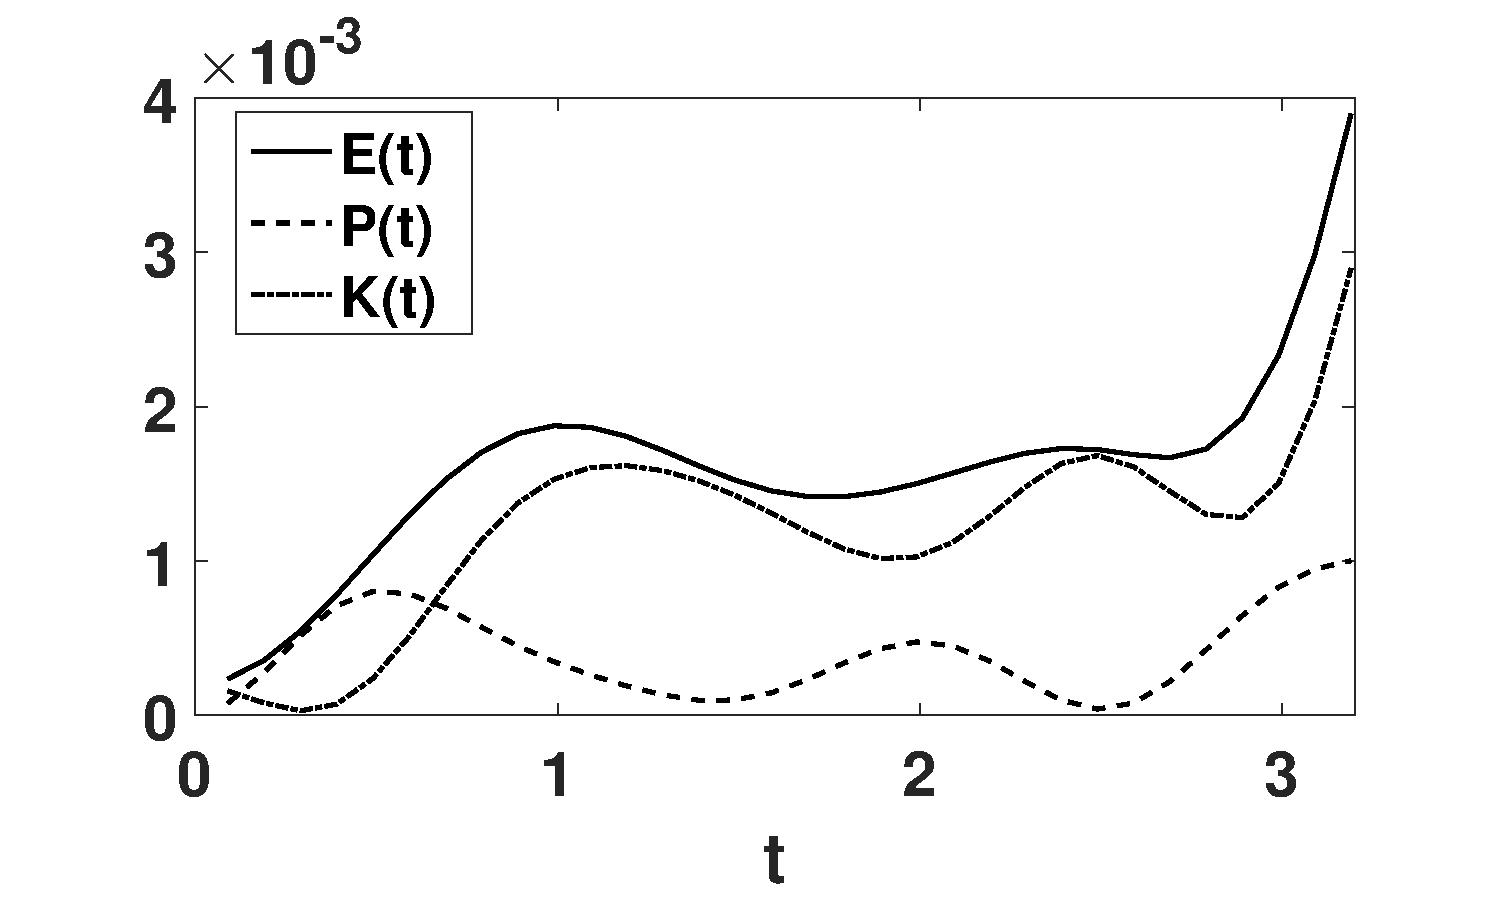
\includegraphics[width=0.5\textwidth]{energy_profile_mu_pt2_F_pt2_ppmm_sym}
\end{tabular}
\caption{\small {\bf PPMM Case}.  Left Panel: Surface energy $E(t)$, potential energy $P(t)$, and kinetic energy, $K(t)$, profiles in response to the motion of four vortices in the CPPMM configuration. Right Panel: Surface energy $E(t)$, potential energy $P(t)$, and kinetic energy, $K(t)$, profiles in response to the motion of four vortices in the EPPMM configuration.  $F=0.2$ and $\mu=0.2$ in both panels, and simulations are run for $0\leq t \leq t_{b}$.}
\label{fig:eprof_ppmm}
\end{figure}

A possible explanation for the more complicated responses of $\delta_{b}$ to $F$, again see Figure \ref{fig:froudecomp_ppmm} (Lower Panels), is that, as seen in Figure \ref{fig:tracksppmm}, while one pair of vortices ends up higher than the other, the other pair still rises closer to the surface.  Thus, the added energy of this secondary pair complicates the ways in which the highest vortices approach the surface, in part then explaining the far greater sensitivity of $\delta_{b}$ to $F$.  However, more work needs to be done to fully understand this phenomena.  

%%%%%%%%%%%%%%%%%%%%%%%%%%%%%%%%%%%%%%%%
\subsection{Four Vortices: Plus/Minus, Minus/Plus}
We now examine the case of four vortices with vortex strengths chosen such that
\[
\Gamma_{1}=1, ~ \Gamma_{2}=-1, ~ \Gamma_{3}=-1,~\Gamma_{4}=1.
\]
We refer to this case as `Plus/Minus, Minus/Plus' or PMMP.  As seen by comparing the left and right panels of Figure \ref{fig:froudecomp_pmmp}, the difference in initial vortex placement again has an impact on the values of $t_{b}$ and $\delta_{b}$.  However, in this case the differences between the CPMMP case and the EPMMP case are far less pronounced compared to the PPMM cases studied above.  There are also clear dependences of $\delta_{b}$ on $\mu$ and $F$ in both cases.  In particular, as with the PM case above, for the larger $\mu$ value, the vortices induce breaking further from the surface with increasing $F$, reflecting the greater sensitivity to vortex strength with increased $\mu$.  
This also corresponds to a similar relationship with the breaking times $t_{b}$, which are longer 
when the vortices induce wave breaking while still further below the surface.  

\begin{figure}[!h]
\centering
\begin{tabular}{cc}
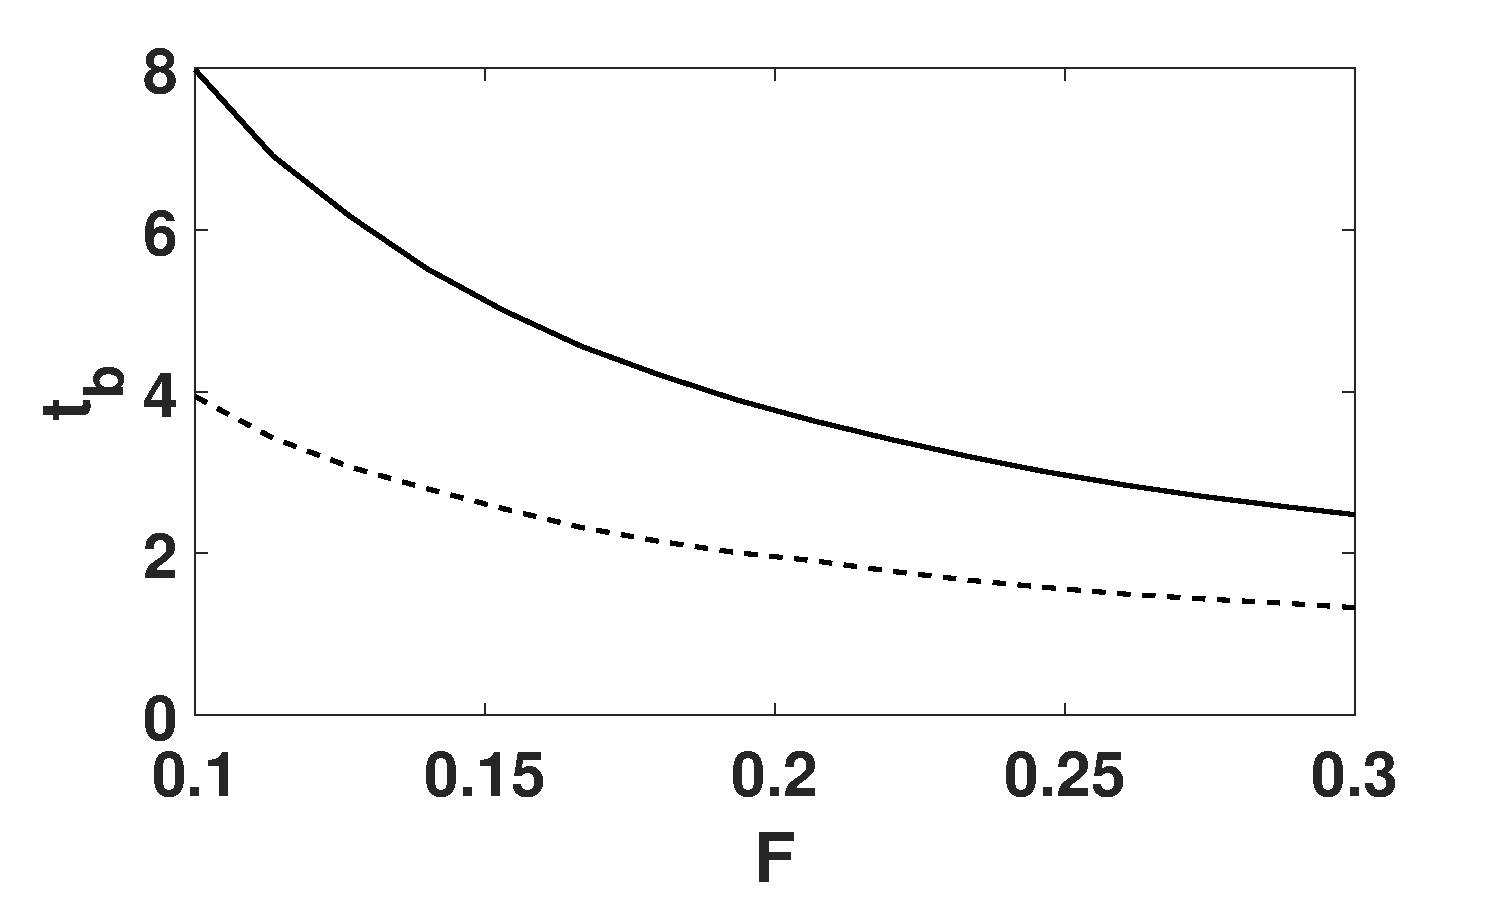
\includegraphics[width=0.5\textwidth]{froude_comp_pmmp} & 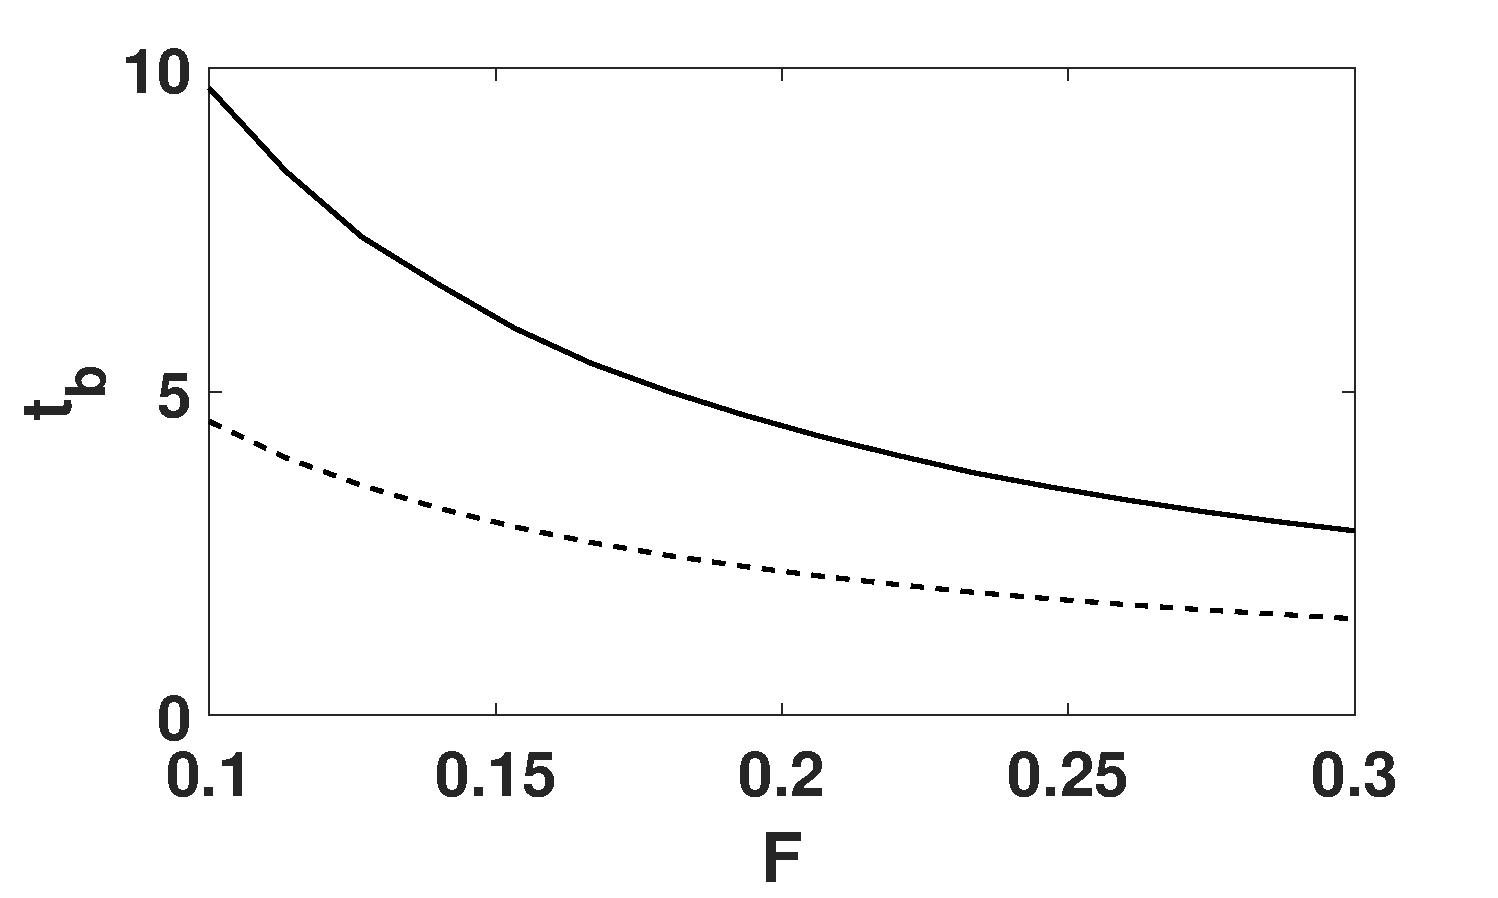
\includegraphics[width=0.5\textwidth]{froude_comp_pmmp_sym}\\
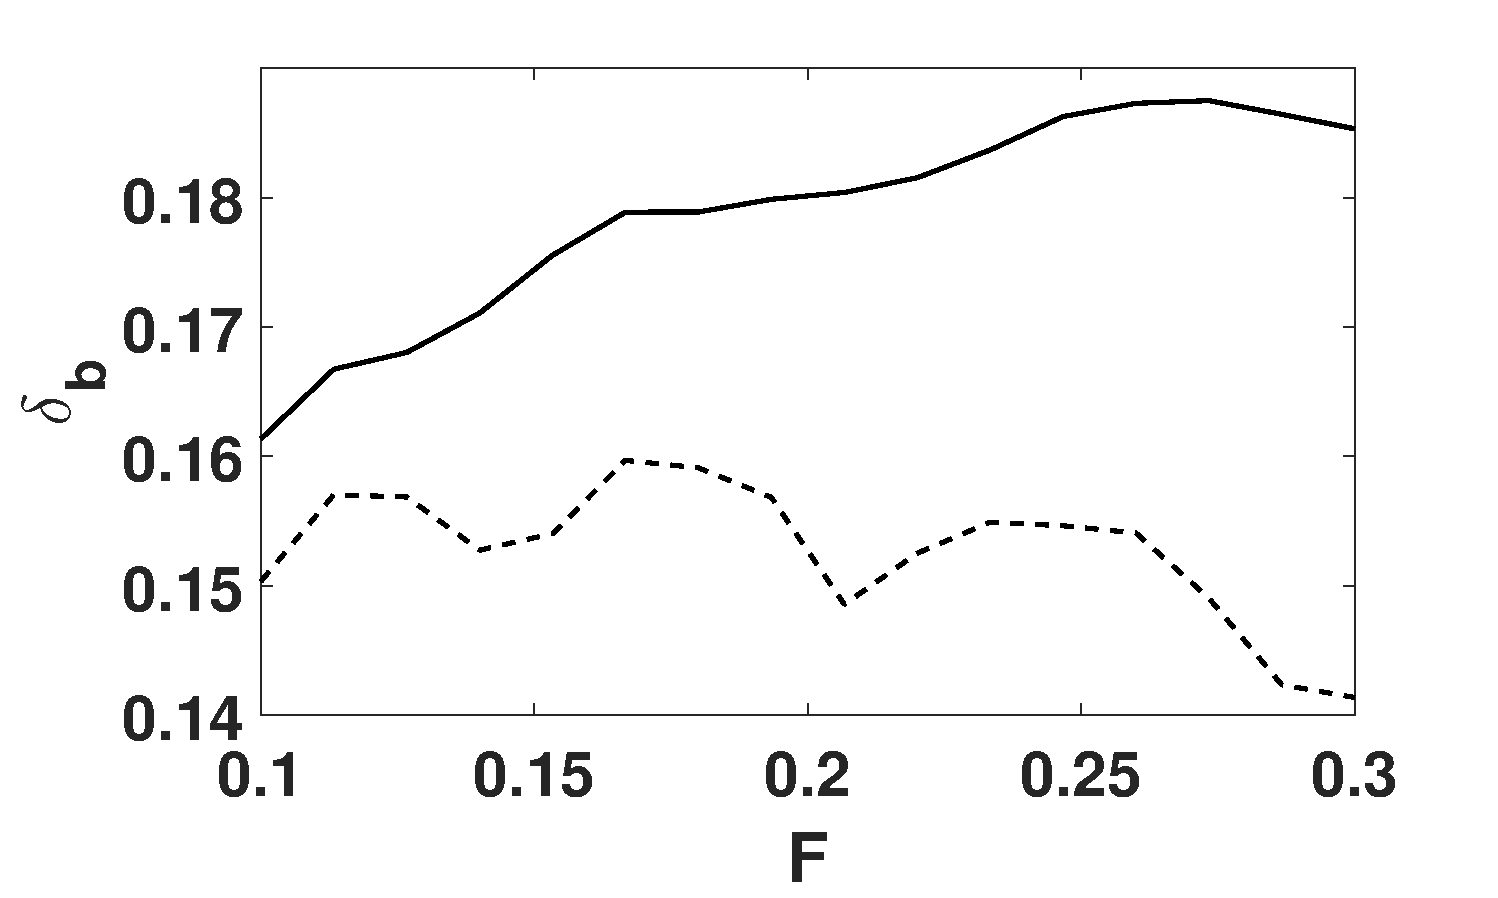
\includegraphics[width=0.5\textwidth]{zmb_pmmp} & 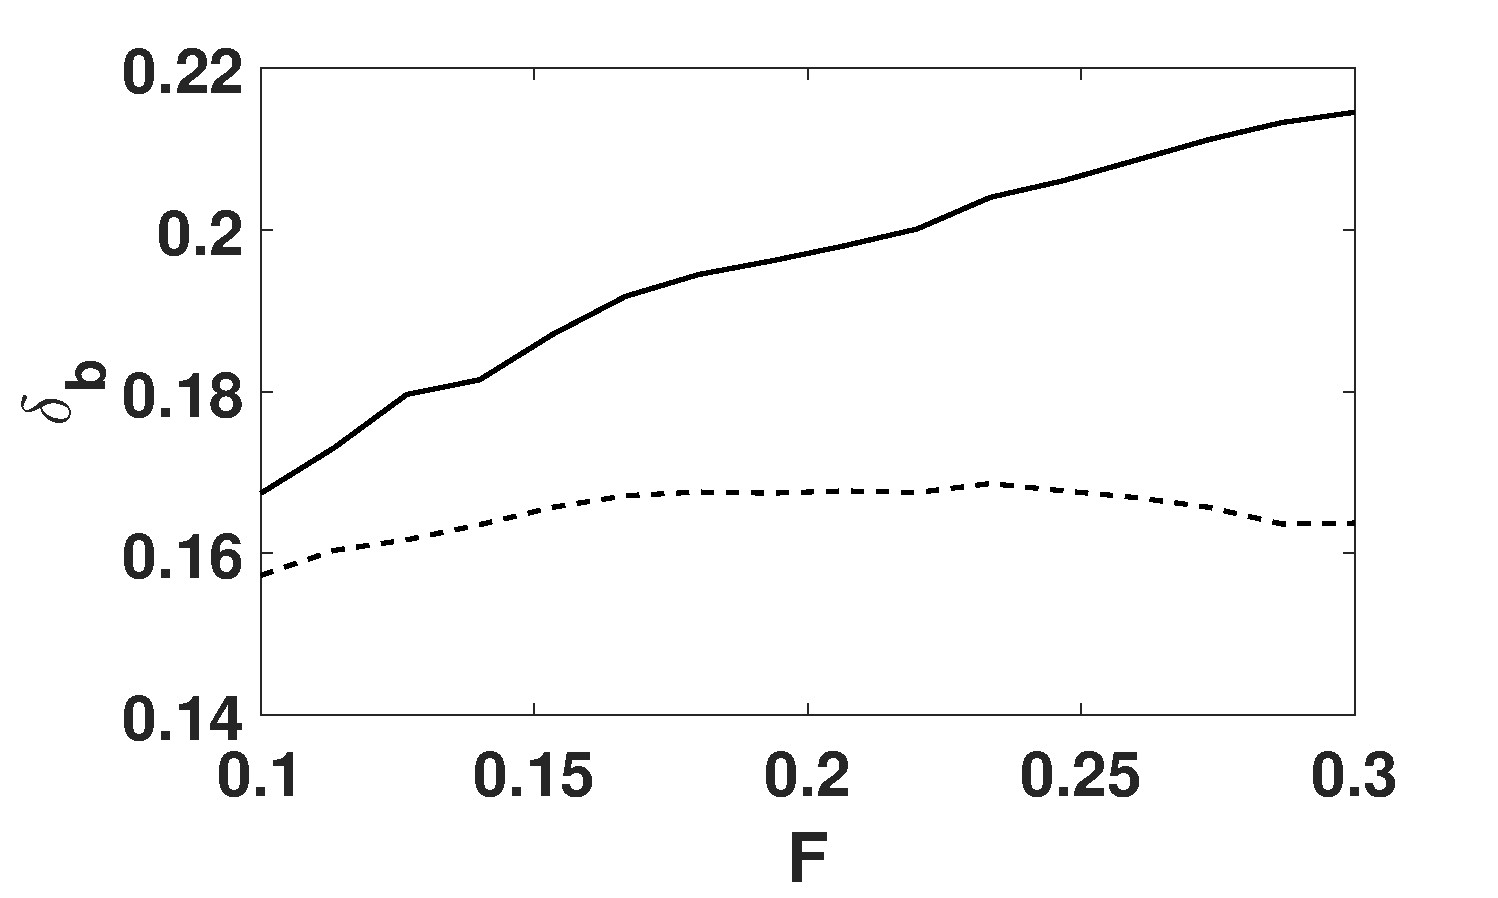
\includegraphics[width=0.5\textwidth]{zmb_pmmp_sym}
\end{tabular}
\caption{\small {\bf PMMP Case}. Upper Panels: Plots of the breaking times $t_{b}$ as a function of Froude number $F$ for $\mu=0.1$ (- -) and $\mu=0.2$ (--).  Lower Panels: Plots of the breaking distances $\delta_{b}$ as a function of Froude number $F$ for $\mu=0.1$ (- -) and $\mu=0.2$ (--). Left Panels: Plots of the breaking time and distance for four vortices starting in the CPMMP configuration.  Right Panels: Plots of the breaking time and distance for four vortices starting in the EPMMP configuration.  $\delta_{b}$ is smaller for the CPMMP case, and $t_{b}$ is longer in the EPMMP case.}
\label{fig:froudecomp_pmmp}
\end{figure}

Again, choosing $F=0.2$ and $\mu=0.2$, we can in part explain the above features by examining the flow dynamics for both the CPMMP and EPMMP cases.  As seen in Figure \ref{fig:surfreppmmp}, $t_{b}$ is roughly the same, and in both cases, the surface response is highly asymmetric, though the EPMMP case induces a higher degree of asymmetry than the CPMMP case.  What is perhaps surprising is that such strong differences in the surface profile can emerge given that the vortex paths are relatively similar; see Figure \ref{fig:trackpmmp}.  This certainly explains the strong similarities seen in Figure \ref{fig:froudecomp_pmmp}.  The strong surface differences then appear to be due to the added sense of rotation seen in the EPMMP vortex path.  We also see in both cases that the right-most vortex pair behaves as in inviscid wall-bounded flows \cite{lamb}.  The energy profiles seen in Figure \ref{fig:eprof_pmmp}     are very similar with $E(t)$ essentially tracking $K(t)$ in similar ways over similar time scales, though there is some small oscillations between $K(t)$, and thus $E(t)$, in the CPMMP case not seen in the EPMMP case. Given the absence of circular motion of the vortices though, there is not significant exchange between $K(t)$ and $P(t)$ in either case.   
\begin{figure}[!h]
\centering
\begin{tabular}{cc}
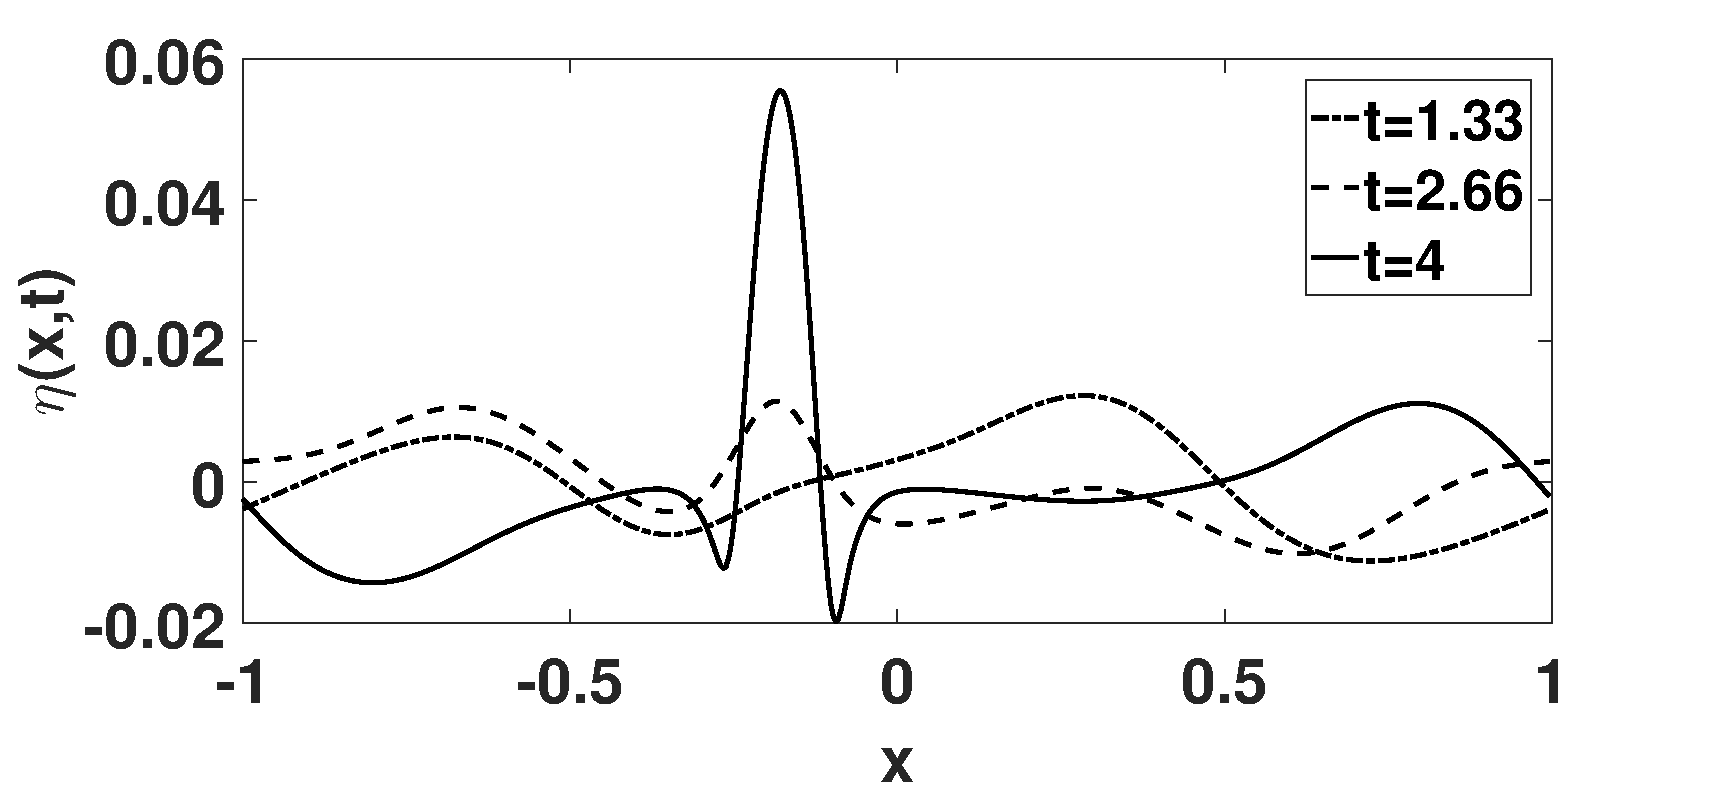
\includegraphics[width=0.5\textwidth]{surf_resp_mu_pt2_F_pt2_pmmp} & 
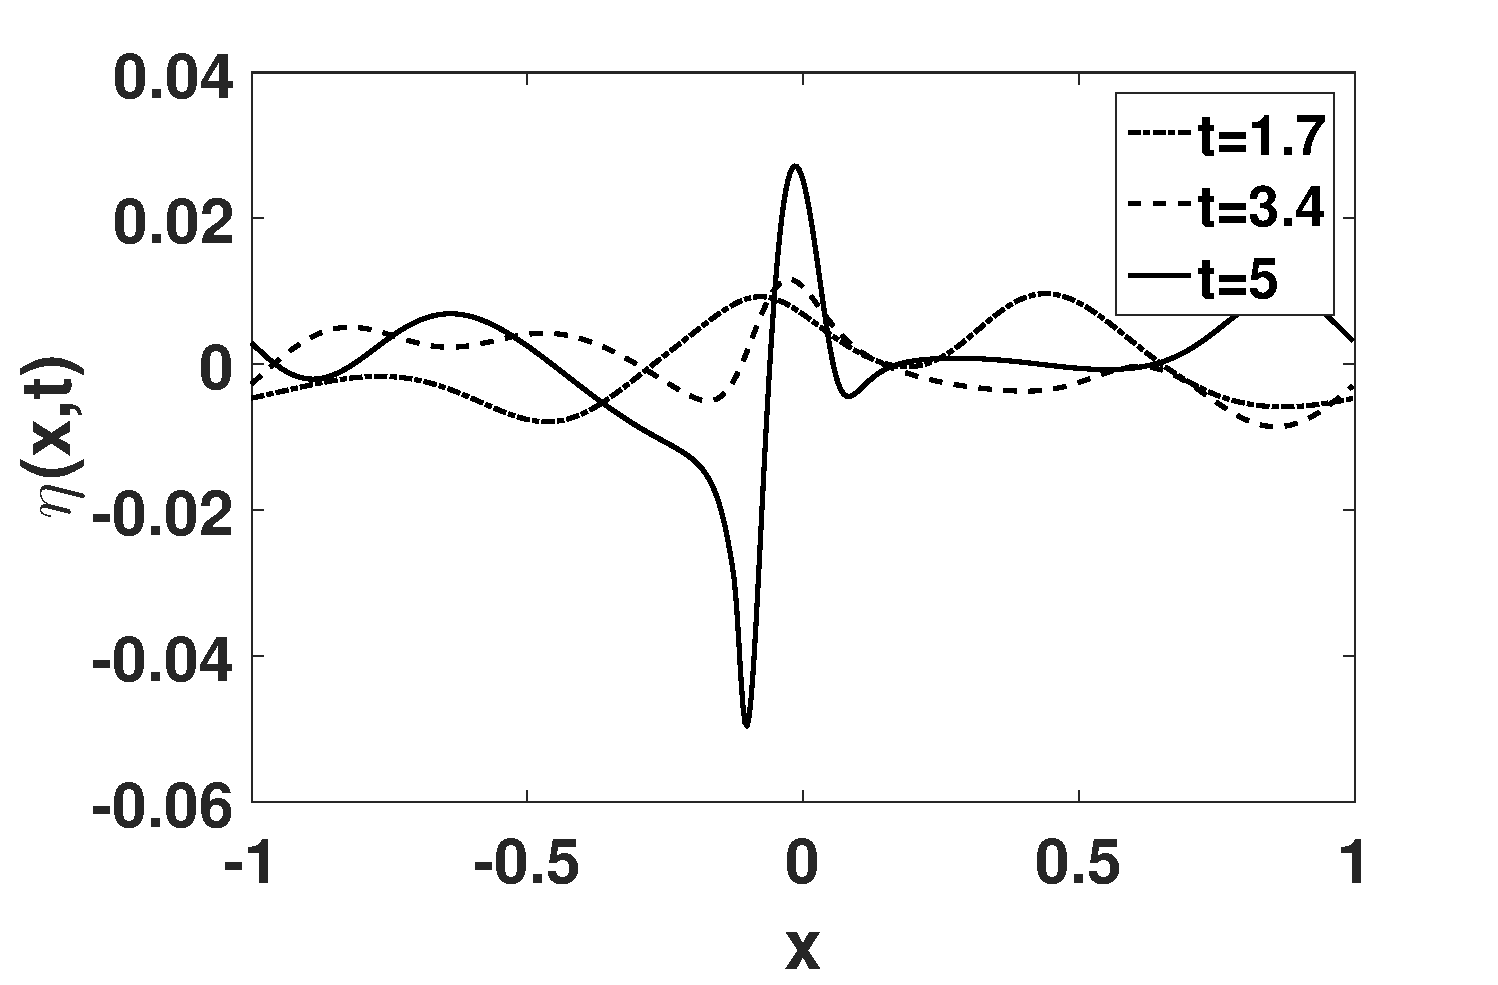
\includegraphics[width=0.5\textwidth]{surf_resp_mu_pt2_F_pt2_pmmp_sym}
\end{tabular}
\caption{\small ({\bf PMMP Case}) Left Panel: Surface response $\eta(x,t)$ over four vortices in the CPMMP configuration. Right Panel: Surface response $\eta(x,t)$ over four vortices in the EPMMP configuration.  $F=0.2$ and $\mu=0.2$ in both panels.}
\label{fig:surfreppmmp}
\end{figure}
%
\begin{figure}[!h]
\centering
\begin{tabular}{cc}
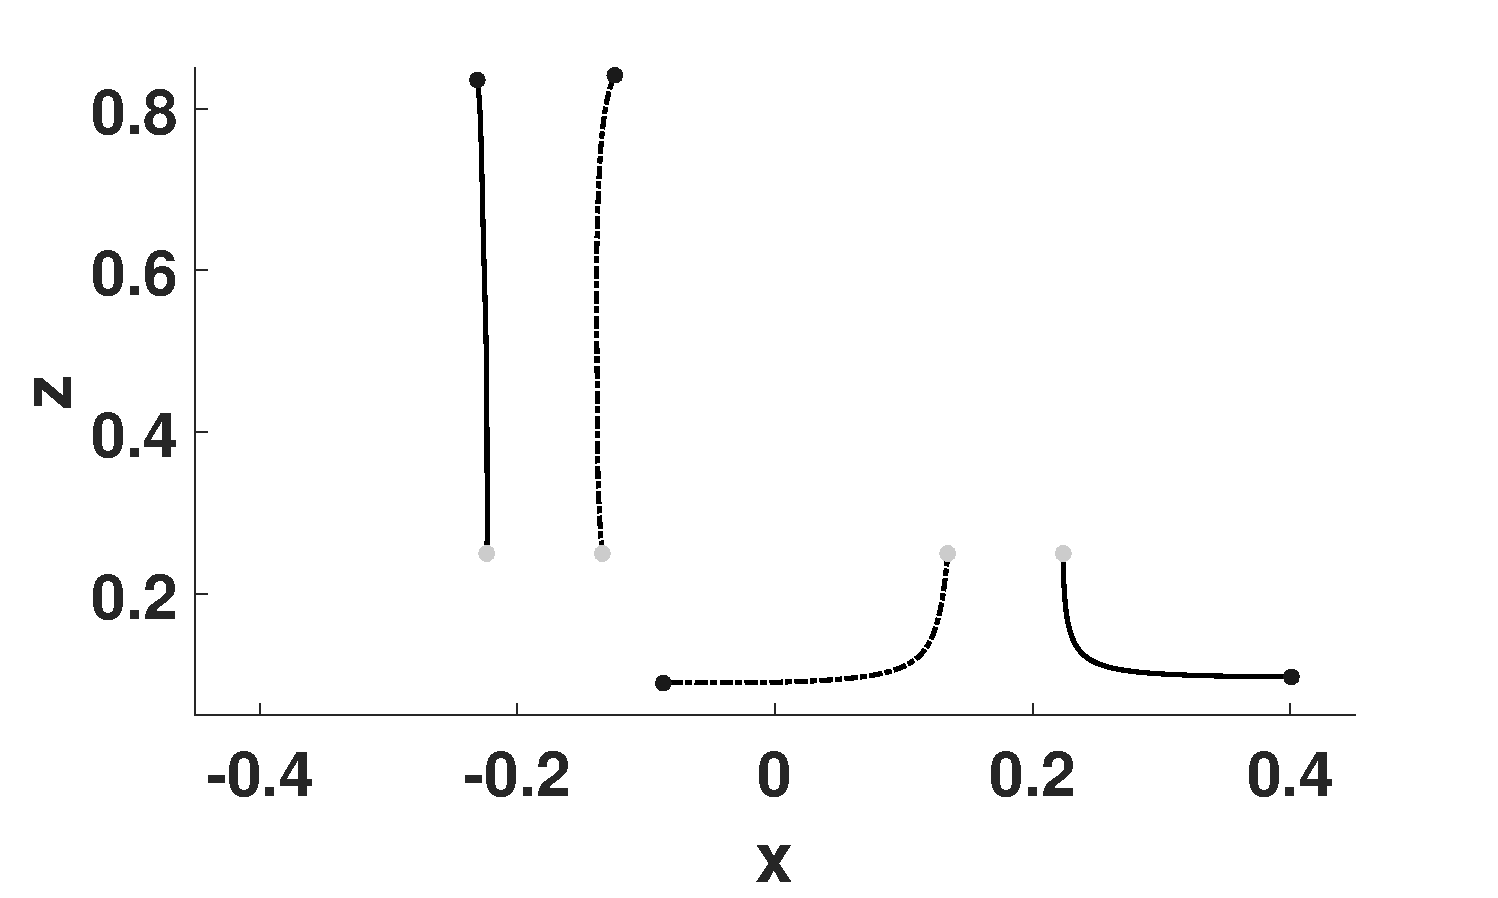
\includegraphics[width=0.5\textwidth]{tracks_F_pt2_tf_4_pmmp} & 
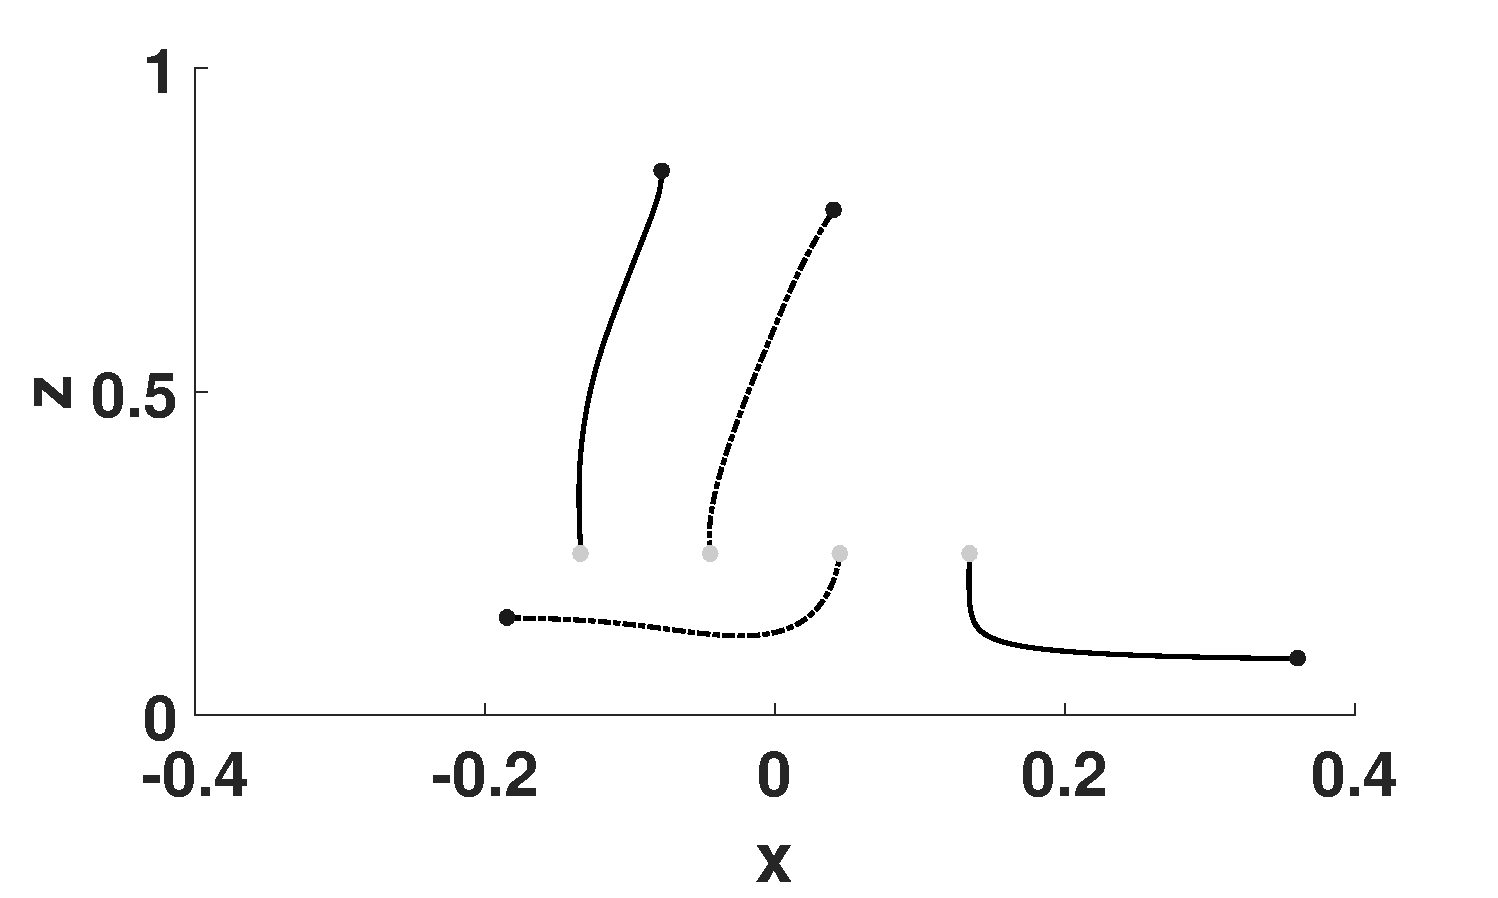
\includegraphics[width=0.5\textwidth]{tracks_F_pt2_tf_5_pmmp_sym}
\end{tabular}
\caption{\small ({\bf PMMP Case}) Left Panel: Vortex paths for four vortices in the CPMMP configuration.  Right Panel: Vortex paths for four vortices in the EPMMP configuration. $F=0.2$ and $\mu=0.2$ in both panels, and simulations are run for $0\leq t \leq t_{b}$.}
\label{fig:trackpmmp}
\end{figure}

\begin{figure}[!h]
\centering
\begin{tabular}{cc}
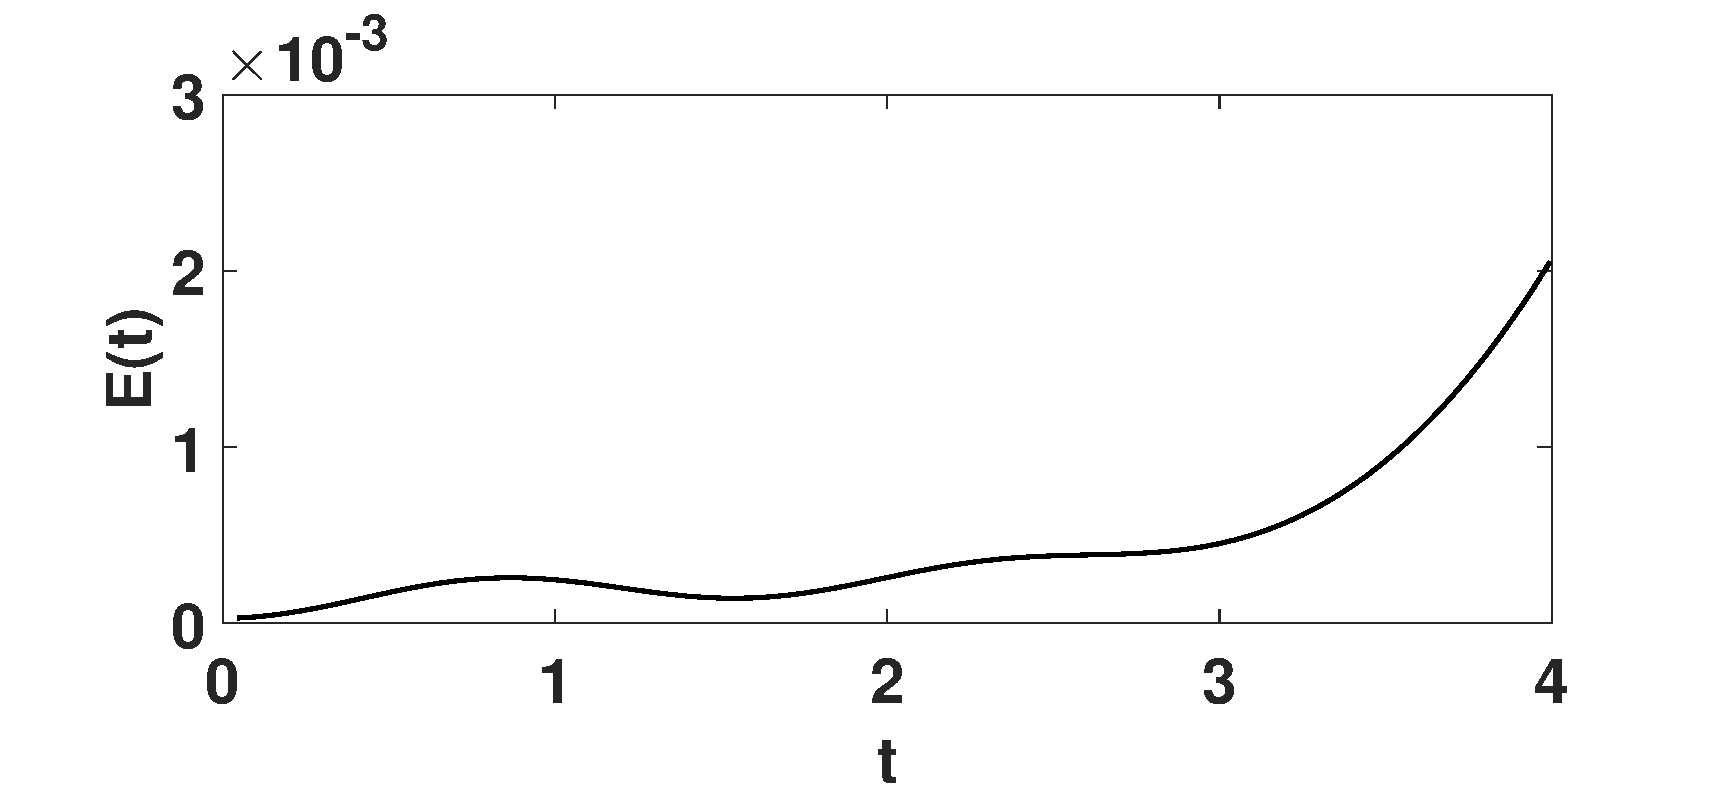
\includegraphics[width=0.5\textwidth]{energy_profile_mu_pt2_F_pt2_pmmp} &
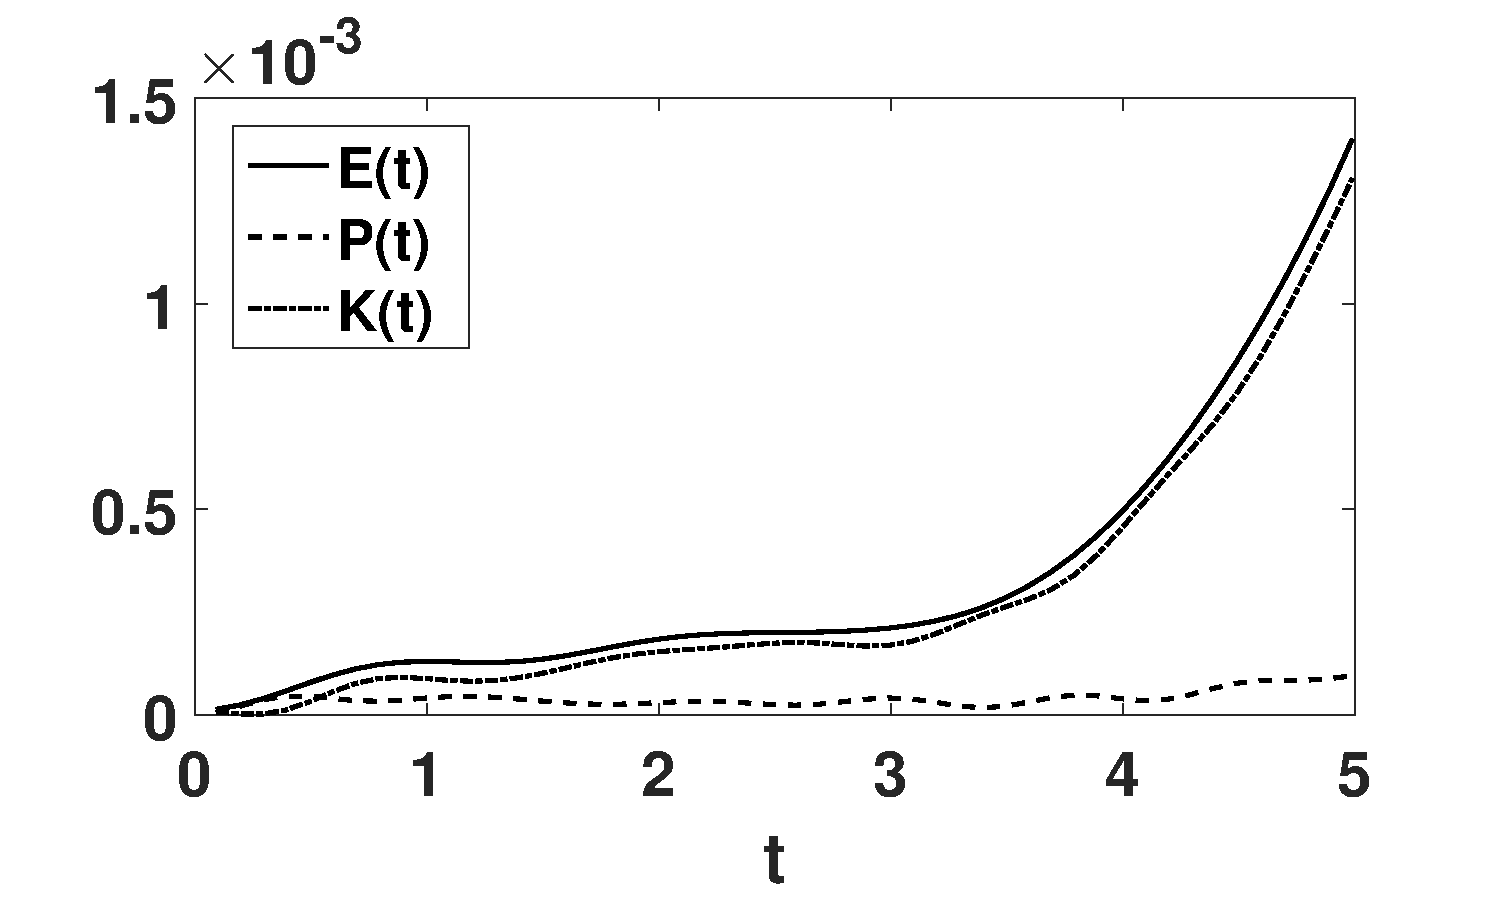
\includegraphics[width=0.5\textwidth]{energy_profile_mu_pt2_F_pt2_pmmp_sym}
\end{tabular}
\caption{\small ({\bf PMMP Case}) Left Panel: Surface energy $E(t)$, potential energy $P(t)$, and kinetic energy, $K(t)$, profiles in response to the motion of four vortices in the CPMMP configuration.  Right Panel: Surface energy $E(t)$, potential energy $P(t)$, and kinetic energy, $K(t)$, profiles in response to the motion of four vortices in the EPMMP configuration.  $F=0.2$ and $\mu=0.2$ in both panels, and simulations are run for $0\leq t \leq t_{b}$.}
\label{fig:eprof_pmmp}
\end{figure}

%%%%%%%%%%%%%%%%%%%%%%%%%%%%%%%%%%%%%%%%
\subsection{Four Vortices: Plus/Minus, Plus/Minus}
Finally, we now look at the case of four vortices, chosen so that
\[
\Gamma_{1}=1,~\Gamma_{2}=-1, ~ \Gamma_{3}=1,~\Gamma_{4}=-1.
\]
Again, in keeping with our convention, this is called the `Plus/Minus,Plus/Minus' or PMPM case.  Similar to the strong differences seen above in the PPMM cases, the left and right panels of Figure \ref{fig:froudecomp_pmpm} show that differences in initial vortex placement have strong effects on $t_{b}$ and $\delta_{b}$.  The CPMPM case breaks in half the time; compare Figure \ref{fig:froudecomp_pmpm} (Top Left Panel) and (Top Right Panel).  Further, in the CPMPM case, the vortices reach nearly identical heights for both $\mu=0.1$ and $\mu=0.2$ across a range of $F$ values; see Figure \ref{fig:froudecomp_pmpm} (Bottom Left Panel).  On this point, the EPMPM case is especially striking.  As seen in Figure \ref{fig:froudecomp_pmpm} (Bottom Right Panel), near $F=0.15$ there is a clear transition in how close the vortices get for $\mu=0.2$, providing the first example of a clear binary classification of flows across a change in parameter value.  However, this transition is also troubling since it shows for $F<.15$ that the $\mu=0.2$ case allows for a closer approach than the $\mu=0.1$ case.    
\begin{figure}[!h]
\centering
\begin{tabular}{cc}
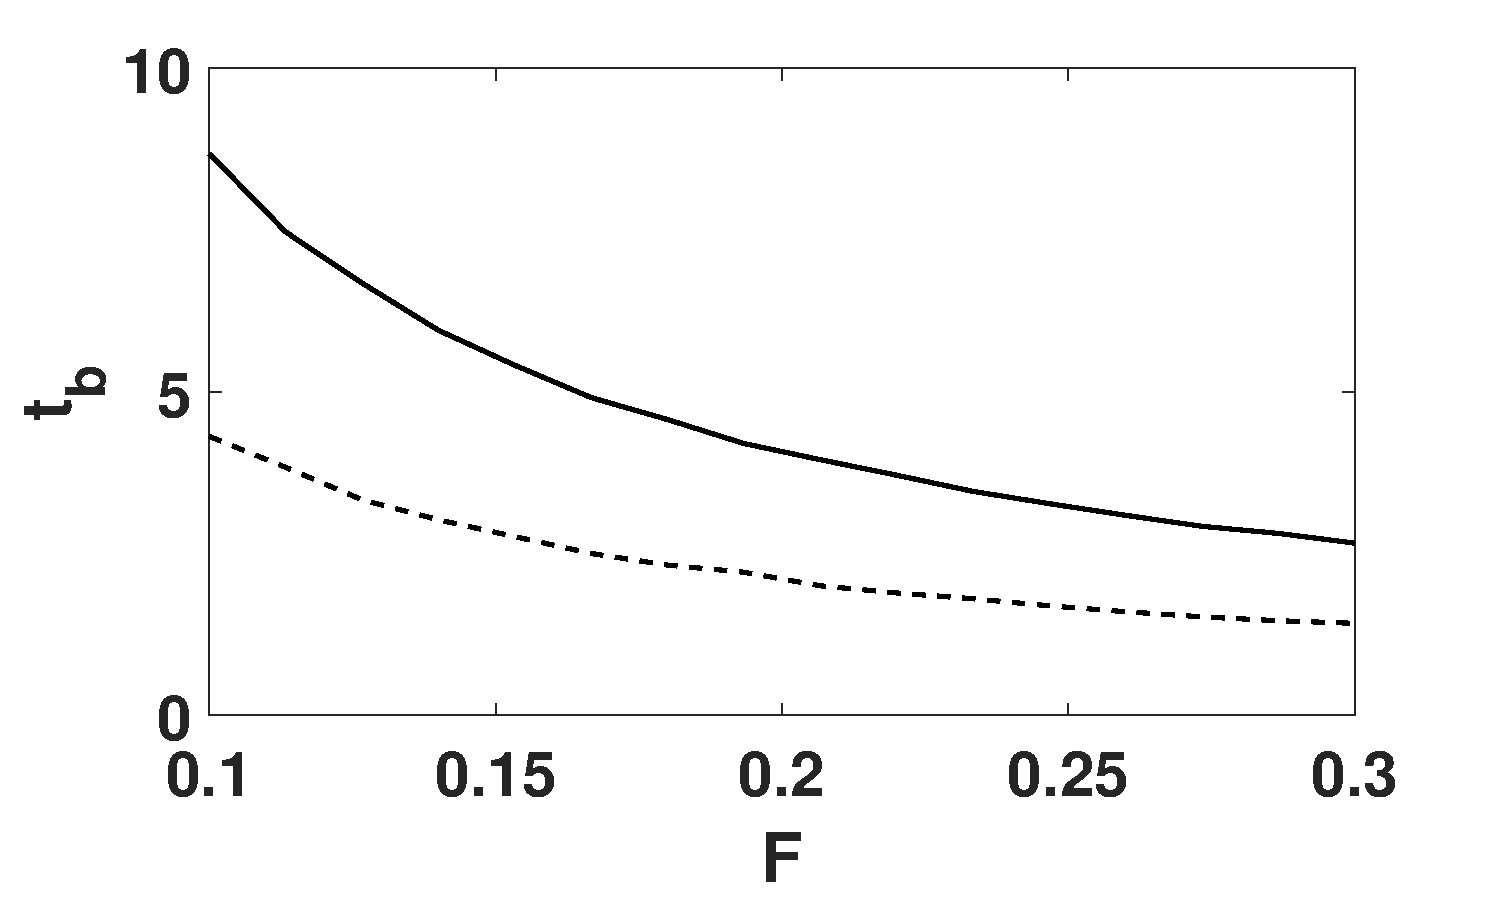
\includegraphics[width=0.5\textwidth]{froude_comp_pmpm} & 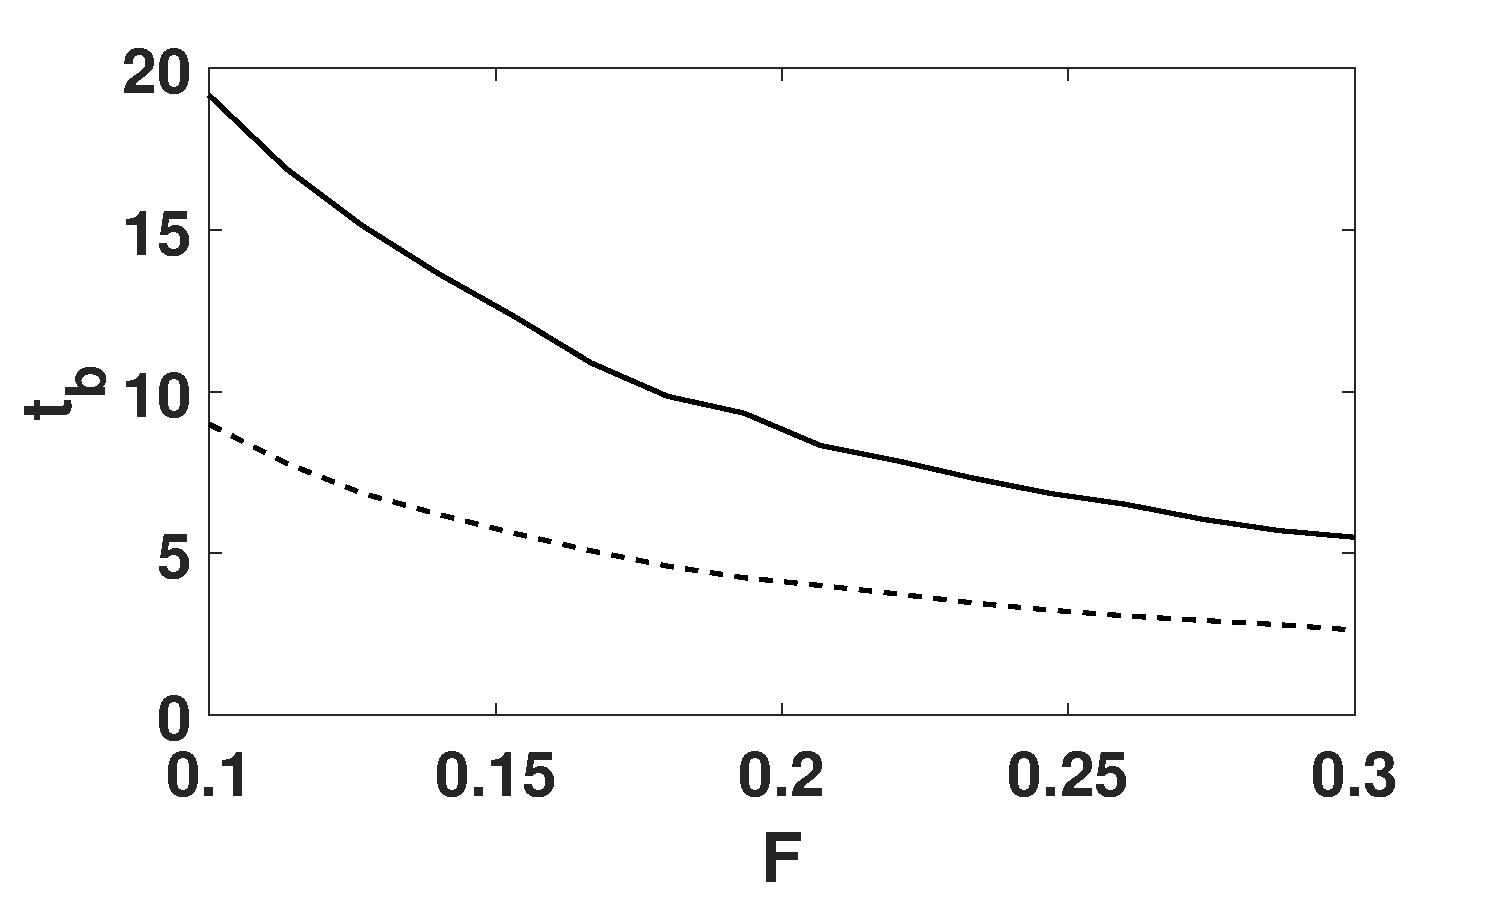
\includegraphics[width=0.5\textwidth]{froude_comp_pmpm_sym}\\
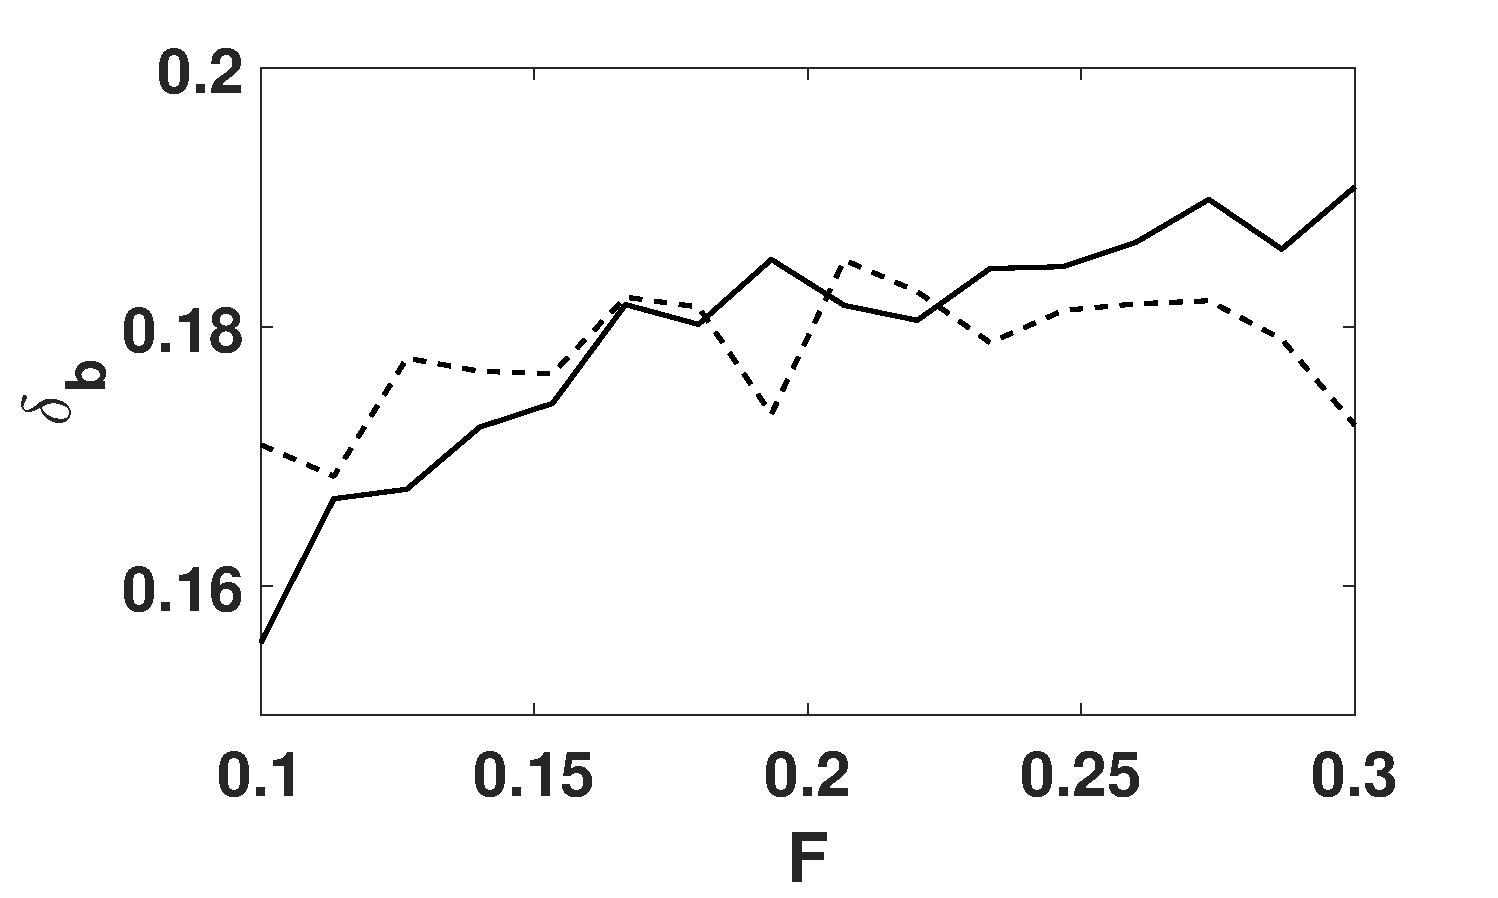
\includegraphics[width=0.5\textwidth]{zmb_pmpm} & 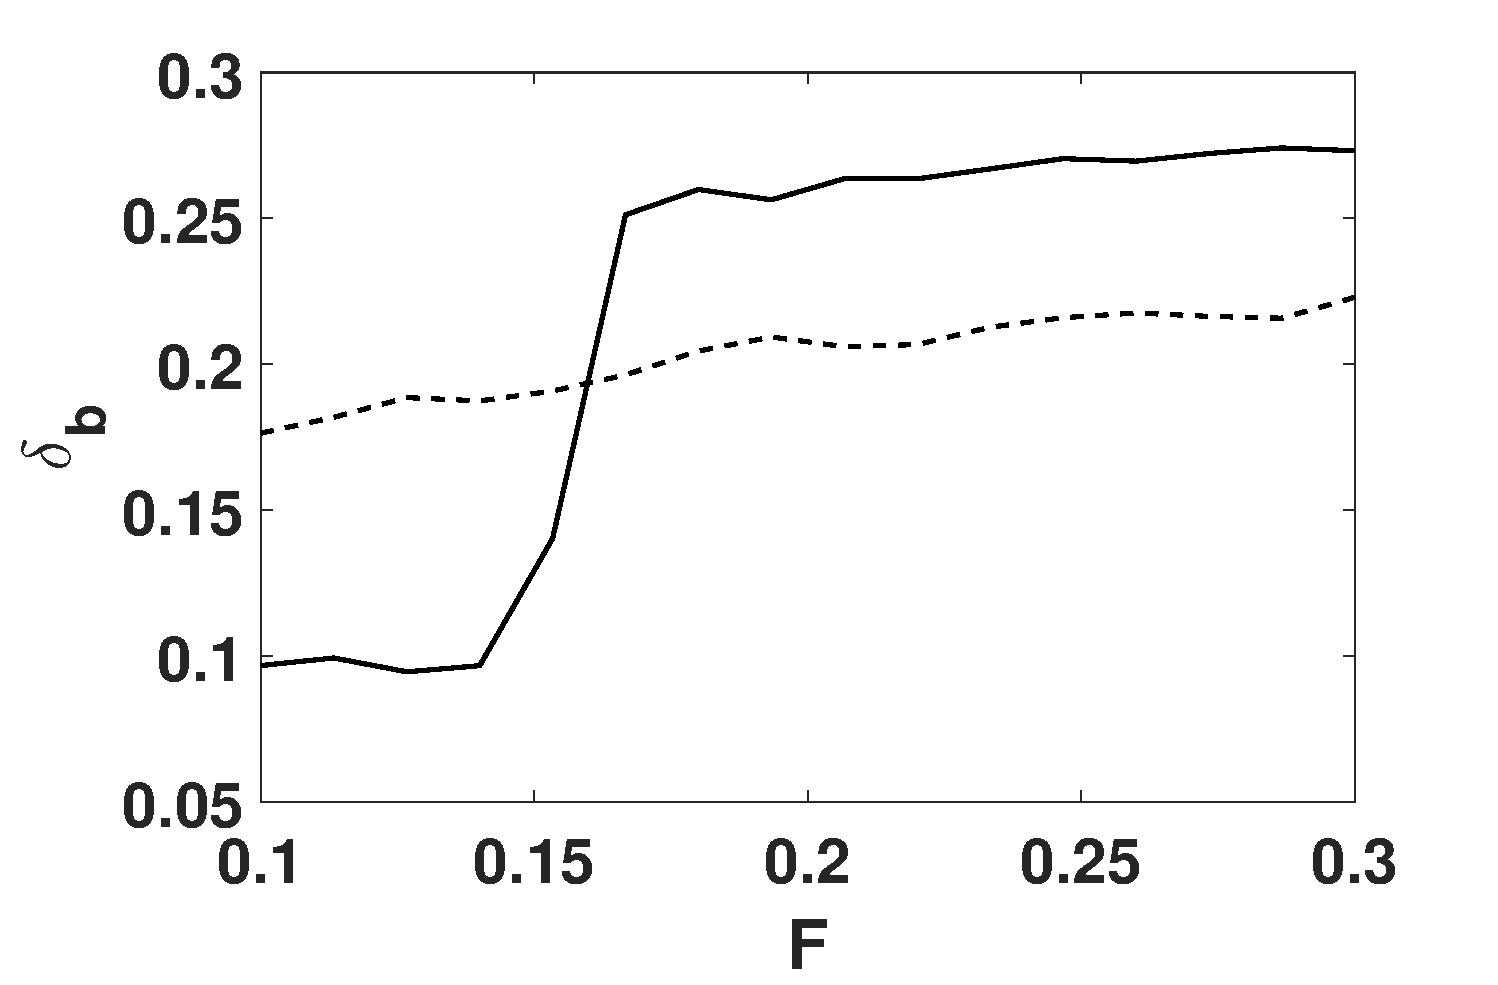
\includegraphics[width=0.5\textwidth]{zmb_pmpm_sym}
\end{tabular}
\caption{\small ({\bf PMPM Case}) Upper Panels: Plots of the breaking times $t_{b}$ as a function of Froude number $F$ for $\mu=0.1$ (- -) and $\mu=0.2$ (--).  Lower Panels: Plots of the breaking distances $\delta_{b}$ as a function of Froude number $F$ for $\mu=0.1$ (- -) and $\mu=0.2$ (--). Left Panels: Plots of the breaking time and distance for four vortices starting in the CPMPM configuration.  Right Panels: Plots of the breaking time and distance for four vortices starting in the EPMPM configuration.  The EPMPM case allows for critical behavior and clear separation in $\delta_{b}$ in terms of $\mu$.}
\label{fig:froudecomp_pmpm}
\end{figure}

Again, taking $F=0.2$ and $\mu=0.2$, we look at particular examples of the CPMPM and EPMPM flows to explain the results in Figure \ref{fig:froudecomp_pmpm} and build intuition through comparison with the previous four vortex cases studied thus far.  What is most striking in this case, and what explains the significant difference in breaking times seen above, is the difference between the vortex paths for the CPMPM and EPMPM case; see Figure \ref{fig:trackpmpm}.  The symmetric initial placement of vortices causes the vortices to follow a more complicated and longer path than seen in the CPMPM case; see Figure \ref{fig:trackpmpm} (Right Panel).  Likewise, the motion of vortices to the edges of the domain in the EPMPM case accounts for the strong amplitude at the boundary domains seen in the surface profile; see Figure \ref{fig:surfrepmpm} (Right Panel).  The plots of $E(t)$ corroborate with this description; see Figure \ref{fig:eprof_pmpm}.  The added complexity of the flow in the EPMPM case again corresponds to larger oscillations in $E(t)$ which largely tracks $K(t)$.  The absence of circular motion in either case though prevents much exchange between $P(t)$ and $K(t)$.  
\begin{figure}[!h]
\centering
\begin{tabular}{cc}
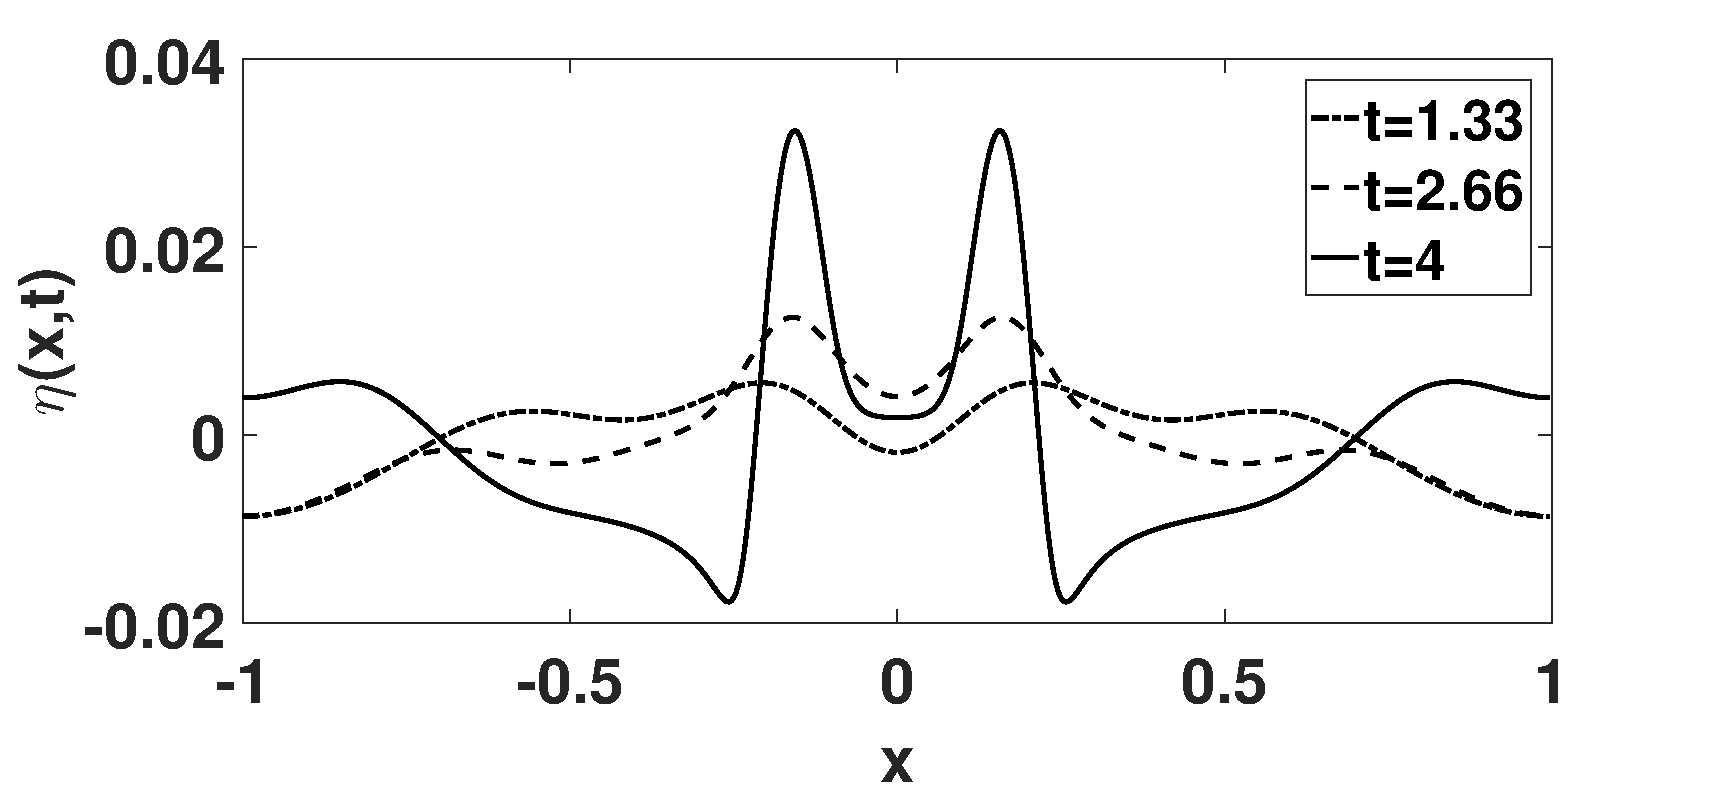
\includegraphics[width=0.5\textwidth]{surf_resp_mu_pt2_F_pt2_pmpm} & 
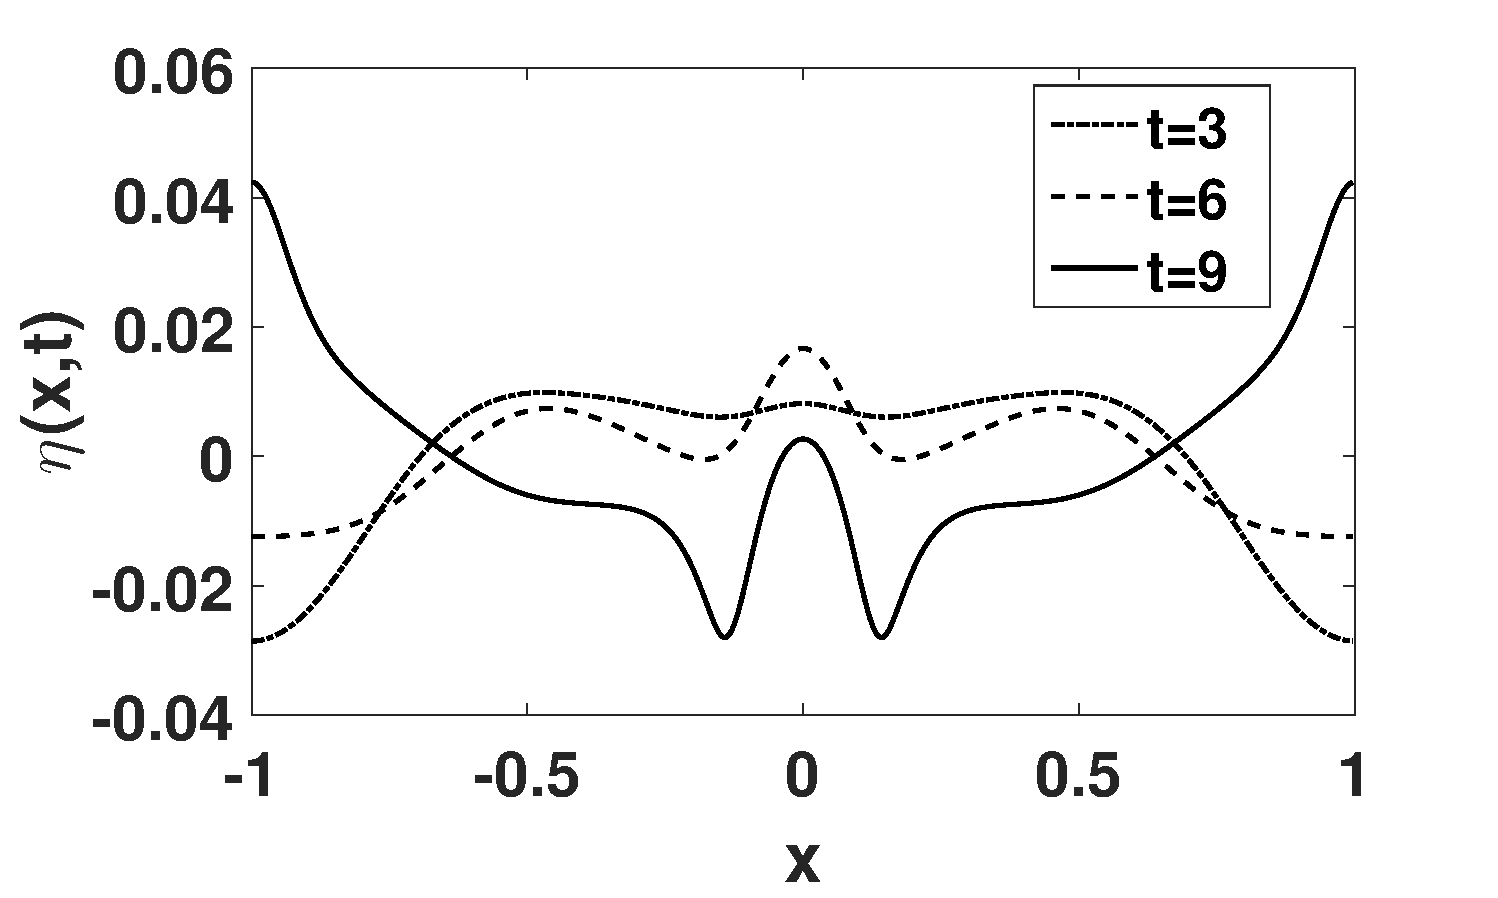
\includegraphics[width=0.5\textwidth]{surf_resp_mu_pt2_F_pt2_pmpm_sym}
\end{tabular}
\caption{\small ({\bf PMPM Case}) Left Panel: Surface response $\eta(x,t)$ over four vortices in the CPMPM configuration. Right Panel: Surface response $\eta(x,t)$ over four vortices in the EPMPM configuration.  $F=0.2$ and $\mu=0.2$ in both panels.}
\label{fig:surfrepmpm}
\end{figure}
%
\begin{figure}[!h]
\centering
\begin{tabular}{cc}
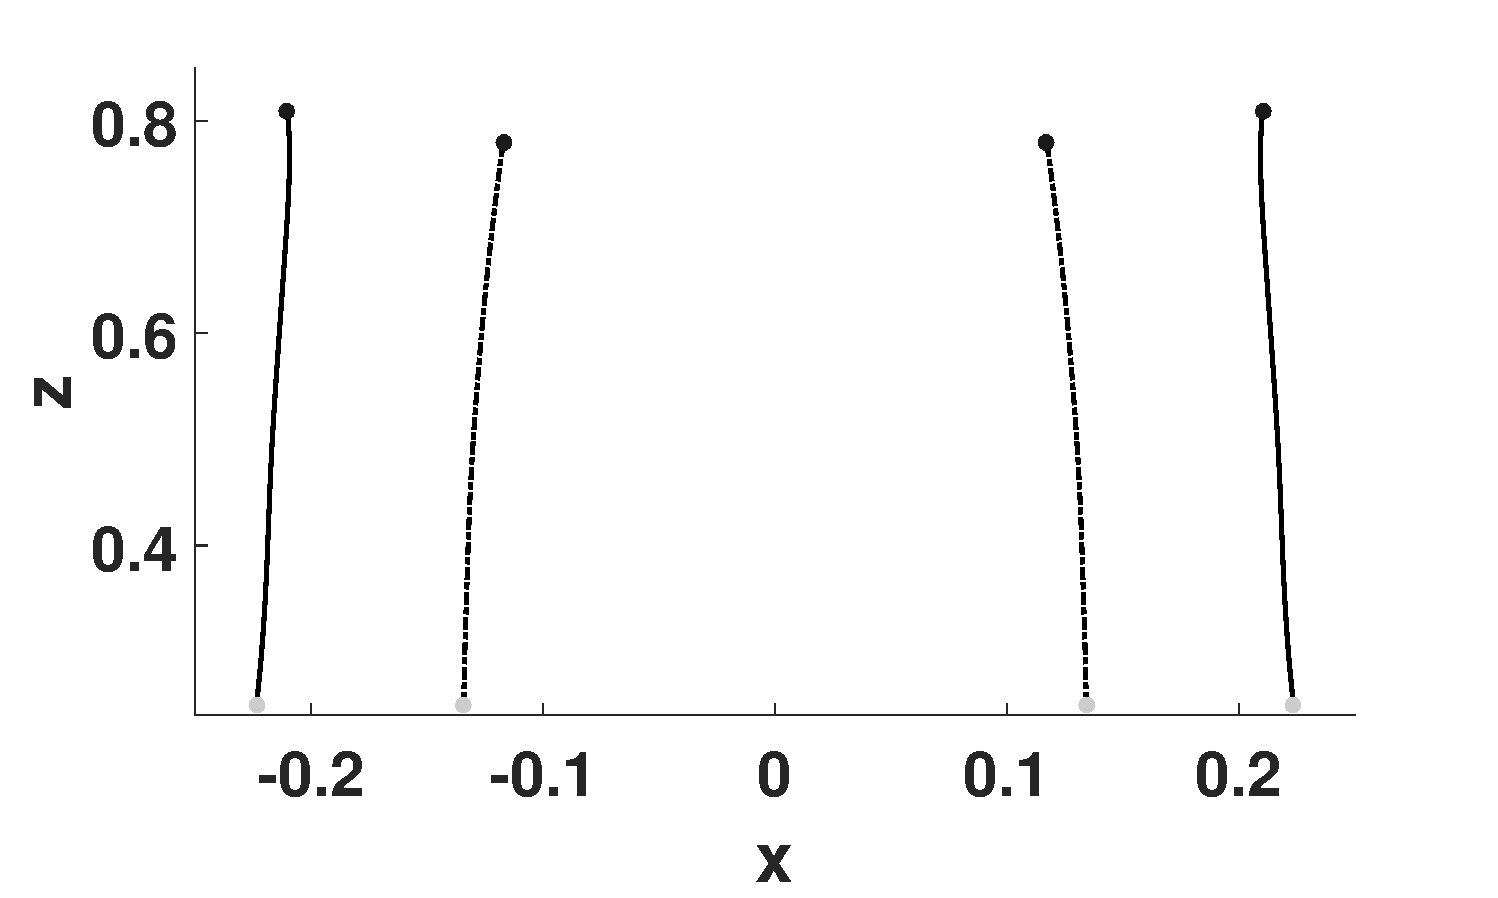
\includegraphics[width=0.5\textwidth]{tracks_F_pt2_tf_4_pmpm} & 
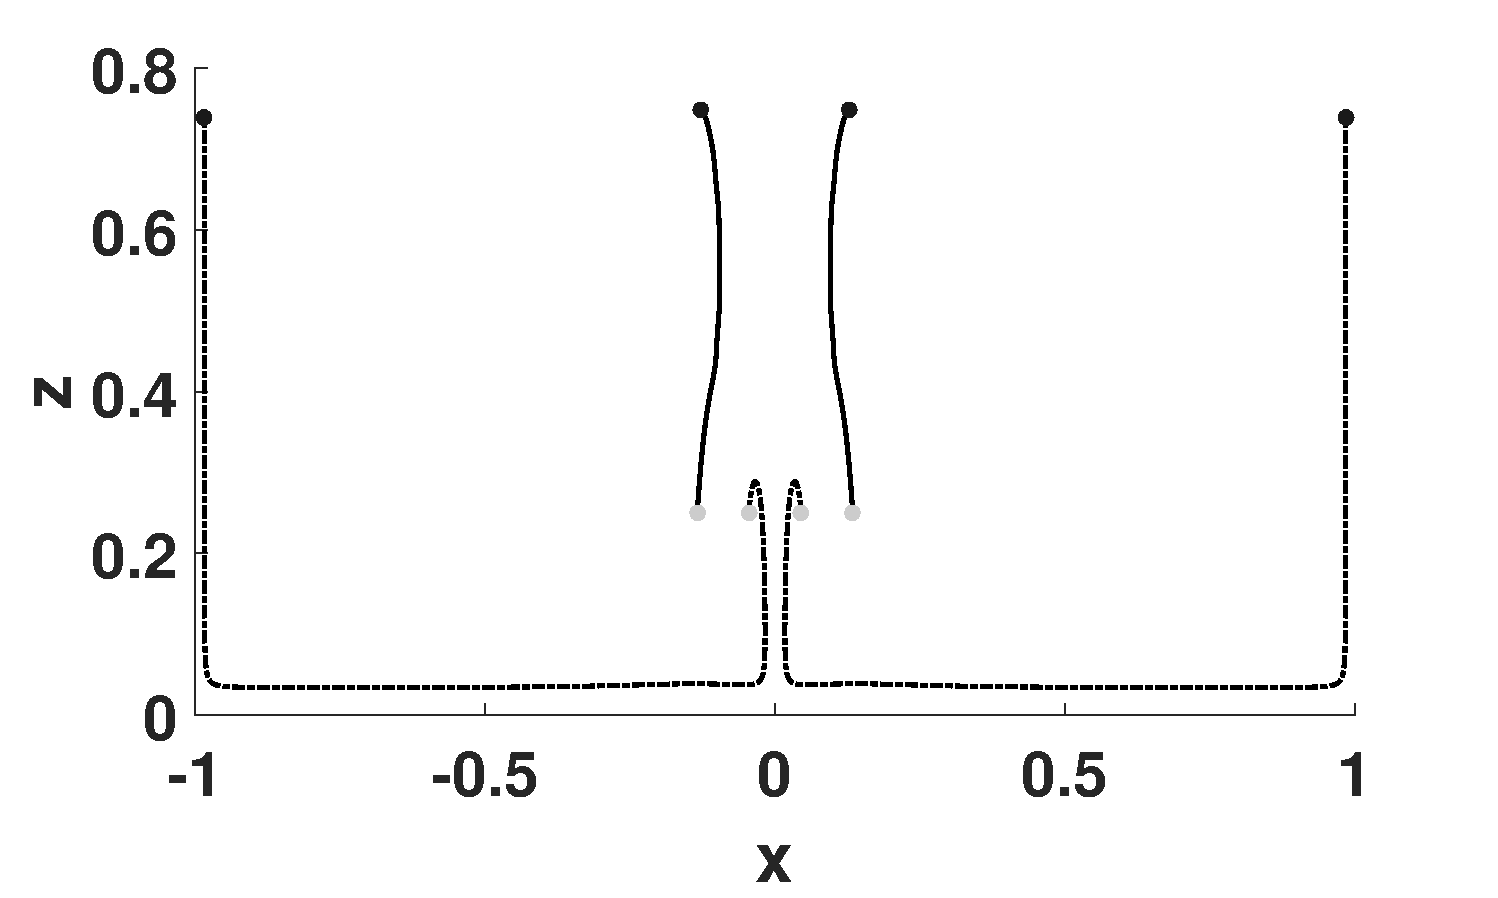
\includegraphics[width=0.5\textwidth]{tracks_F_pt2_tf_9_pmpm_sym}
\end{tabular}
\caption{\small  ({\bf PMPM Case}) Left Panel: Vortex paths for four vortices in the CPMPM configuration.  Right Panel: Vortex paths for four vortices in the EPMPM configuration. $F=0.2$ and $\mu=0.2$ in both panels, and simulations are run for $0\leq t \leq t_{b}$.}
\label{fig:trackpmpm}
\end{figure}

\begin{figure}[!h]
\centering
\begin{tabular}{cc}
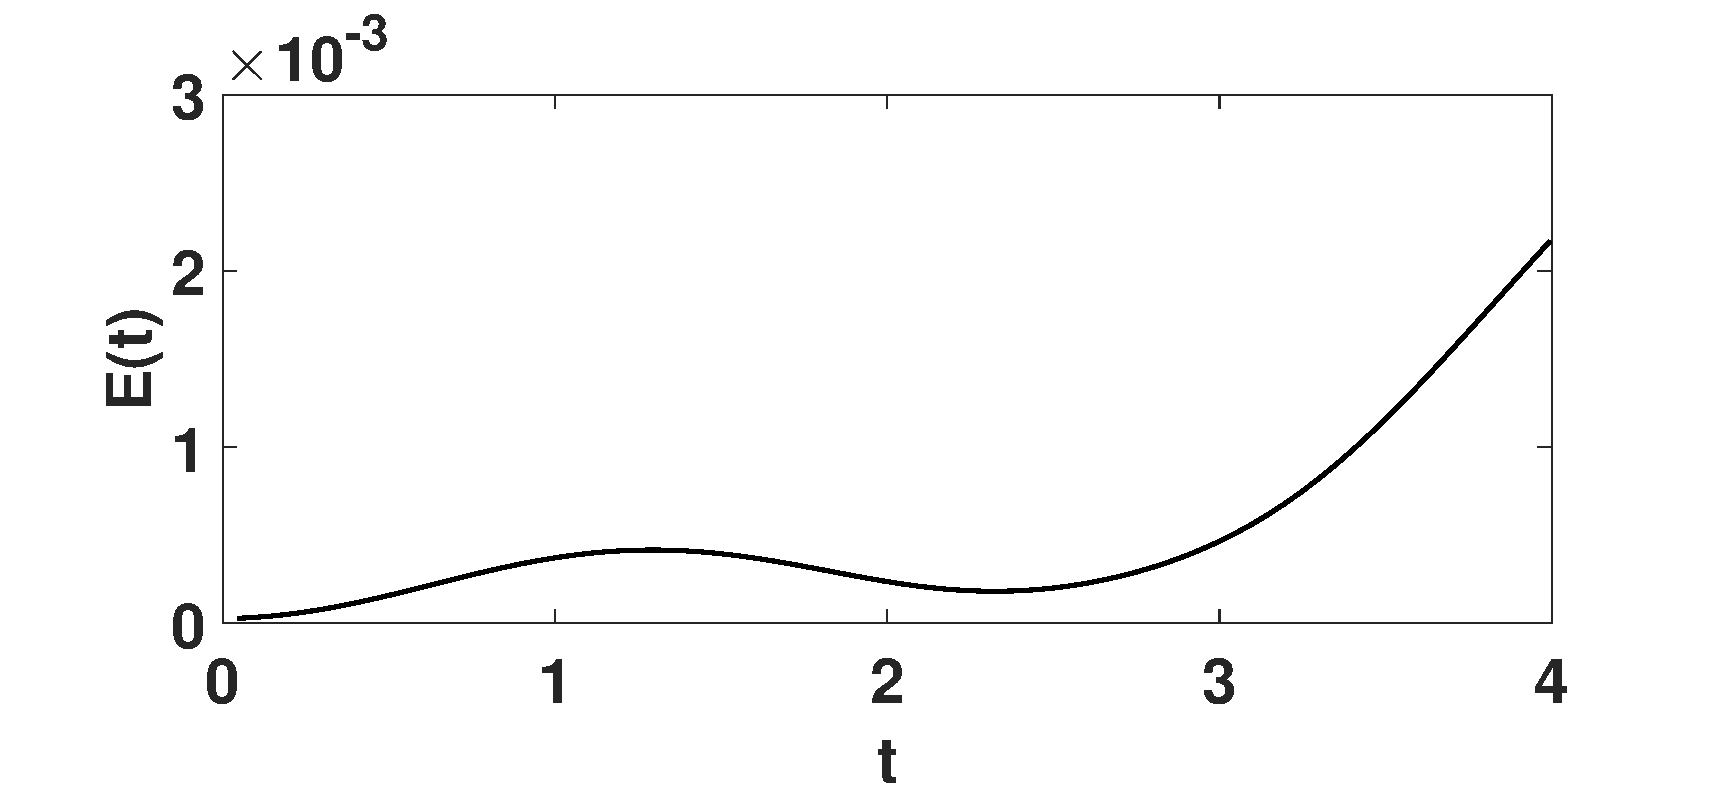
\includegraphics[width=0.5\textwidth]{energy_profile_mu_pt2_F_pt2_pmpm} &
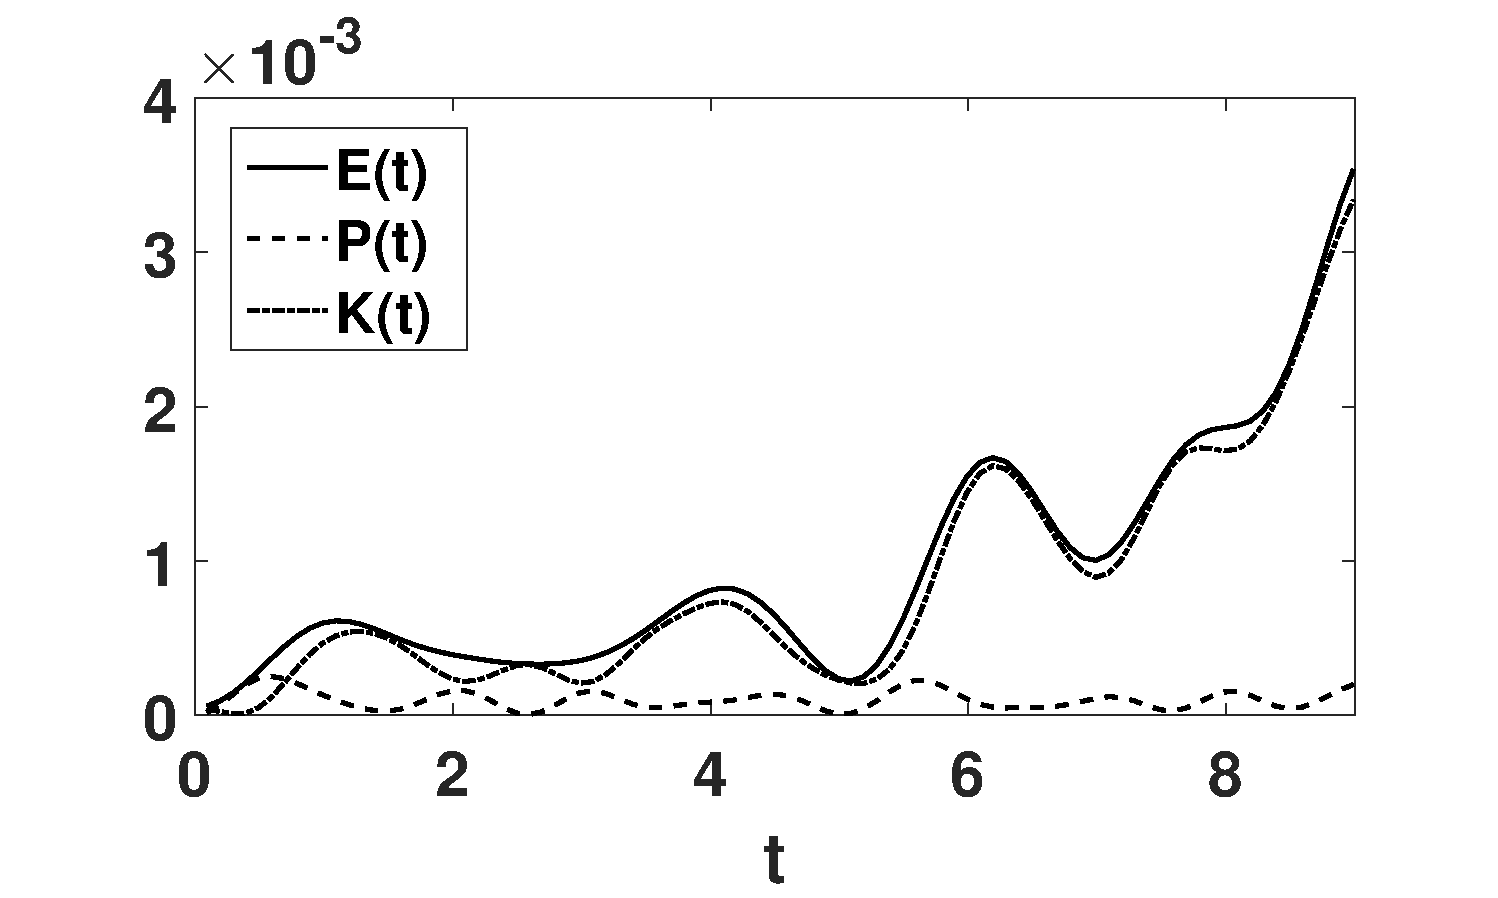
\includegraphics[width=0.5\textwidth]{energy_profile_mu_pt2_F_pt2_pmpm_sym}
\end{tabular}
\caption{\small ({\bf PMPM Case}) Left Panel: Surface energy $E(t)$, potential energy $P(t)$, and kinetic energy, $K(t)$, profiles in response to the motion of four vortices in the CPMPM configuration. Right Panel: Surface energy $E(t)$, potential energy $P(t)$, and kinetic energy, $K(t)$, profiles in response to the motion of four vortices in the EPMPM configuration.  $F=0.2$ and $\mu=0.2$ in both panels, and simulations are run for $0\leq t \leq t_{b}$.}
\label{fig:eprof_pmpm}
\end{figure}

%%%%%%%%%%%%%%%%%%%%%%%%%%%%%%%%%%%%%%%%%%%%%%%%%%%%%%%%%%%%%%%%%%%%%%%%%%%%%%%%
\section{Conclusions and Future Work}
In this paper, we have derived a nonlinear integro-differential system of equations in terms of surface variables and vortex positions alone which allows for the ready development of numerical simulations and asymptotic approximations.  While being able to recreate results similar to those known for two counter-propagating vortices over infinite depth, our approach allows for arbitrary, non-symmetric vortex configurations to be simulated which also take into account the influence of bottom boundaries of the fluid. The presence of bottom boundaries was shown to strongly influence dynamics.  In particular, the vortices are able to rise to the surface at a faster rate than in the deep-water case, leading for example to breaking like phenomena on much shorter time scales than previously reported for deep water flows.  

Further, since we allow for more complicated multi-vortex motion, more complicated surface profiles and vortex paths were observed. In particular, it was found that the arrangement of vortices of positive and negative strength has a major effect on the dynamics.  Likewise, ready classifications into sub or super critical behavior do not seem appropriate for these more complicated cases.  Instead, the range of nonlinear phenomena depends heavily on parameter choices and initial vortex positions.  This hints at the as yet unexplored intricacies of simulating the interactions between surface waves and eddies in more complicated fluid environments.  This is a direction of future work which will build on the results in this paper. \\\\

%For instance, in the Plus/Plus, Minus/Minus configuration shown in Figure \ref{fig:surfrepppmm}, the identical sense of rotation amplifies the vorticity of the individual vortices, and the vortices are tracing out orbiting trajectories as the rise to near the surface.  While the free surface stays symmetric in this case, in the Plus/Minus, Minus/Plus configuration, the surface profile becomes strongly asymmetric after a relatively short time. Finally, in the Plus/Minus, Plus/Minus configuration, the vorticity of these pairs seems to be equalized, leading to near linear vortex trajectories and symmetric surface profiles such as shown in Figure \ref{fig:surfreppmpm}.  The simulation of interactions between surface waves and eddies in more complicated fluid environments is a direction of future work which will build on the results in this paper.        
%%%%%%%%%%%%%%%%%%%%%%%%%%%%%%%%%%%%%%%%%%%%%%%%%%%%%%%%%%%%%%%%%%%%%%%%%%%%%%%%%%

\noindent
{\bf Acknowledgments:}
This work was supported in part by the Research Council of Norway 
through grant no. 213474/F20.


\section{Appendix}
\subsection{Derivation of Bulk-Potential Equation \label{deriv}}
To derive Equation \eqref{blkeq}, in order to have well-defined integrands, we first use the auxiliary harmonic function
\[
\psi_{M,j}(x,z,t) = - \frac{1}{4\pi}\sum_{m=-M}^{M} \left( \mbox{ln}\left( \tilde{x}_{j,m}^{2} + \tilde{z}_{j,-}^{2}  \right) + \mbox{ln}\left( \tilde{x}_{j,m}^{2} + \tilde{z}_{j,+}^{2} \right)\right).
\]
Our choice of auxiliary harmonic function ensures that $\p_{z}\psi_{M,j}(x,0,t)=0$, while avoiding the analytic issues of whether the above sum converges as $M\rightarrow \infty$.  Taking $D$ to be the fluid domain and using Green's third identity, we have that 
\[
\tilde{\phi}_{x}(x_{j},z_{j},t) =  \oint_{\p D} \left(\psi_{M,j}\p_{\hat{{\bf n}}}\tilde{\phi}_{x}-\tilde{\phi}_{x}\p_{\hat{{\bf n}}}\psi_{M,j} \right) ds,
\]
where $\hat{{\bf n}}$ is an outward pointing unit normal vector along the path $\p D_{\epsilon}$.  Note, if $\tilde{\phi}$ is harmonic, then so are all of its partial derivatives.  Defining
\[
g_{M}(x,z,t) = \psi_{M,j}\p_{\hat{{\bf n}}}\tilde{\phi}_{x}-\tilde{\phi}_{x}\p_{\hat{{\bf n}}}\psi_{M,j},
\]
We can then decompose the line integral such that 
\begin{align*}
\oint_{\p D} g_{M}(x,z,t) ds = & \int_{-L}^{L}g_{M}(x,\eta(x,t)+H,t) (1+\eta_{x}^{2})^{1/2}dx \\
& + \int_{0}^{\eta(L,t)+H} \left(g_{M}(L,z,t) + g_{M}(-L,z,t)\right) dz.  
\end{align*}

We now look at letting $M\rightarrow\infty$.  As defined, $\psi_{M,j}$ does not have a well defined limit, however, its derivatives are well defined in this limit, and as we show, it is well behaved along boundaries.  To see this, along $z = \eta(x,t) + H$, we have that 
\[
g_{M}(1+\eta_{x}^{2})^{1/2} = \left.\left(\psi_{M,j}\left(- \eta_{x}\tilde{\phi}_{xx}+\tilde{\phi}_{xz}\right)-\tilde{\phi}_{x}\left(-\eta_{x}\p_{x}\psi_{M,j}+\p_{z}\psi_{M,j}\right) \right)\right|_{z= \eta+H}.
\]
Using $\tilde{\phi}_{xx} = -\tilde{\phi}_{zz}$, we get the identity
\[
\p_{x}\left(\tilde{\phi}_{z}(x, \eta+H,t) \right) = -\eta_{x}\tilde{\phi}_{xx} + \tilde{\phi}_{xz}.
\]
Thus, by integration by parts and using the fact that $\tilde{\phi}(x,z,t)$ and its derivatives are assumed to be periodic in $x$, we have that 
\begin{align*}
\int_{-L}^{L}g_{M}(x,\eta(x,t)+H,t) (1+\eta_{x}^{2})^{1/2}dx = & -\int_{-L}^{L} \left.\left(\tilde{\phi}_{z}\psi^{(1)}_{M,j}+\tilde{\phi}_{x}\psi^{(2)}_{M,j}\right)\right|_{z=\eta+H}dx \\
& + \tilde{\phi}_{z}(L,\eta+H,t)\psi^{(\delta)}_{M,j}(\eta+H,t),
\end{align*}
where
\begin{align*}
\psi^{(1)}_{M,j}(x,t) = \left.\p_{x}\psi_{M,j}+ \eta_{x}\p_{z}\psi_{M,j}\right|_{z=\eta+H}, \\
\psi^{(2)}_{M,j}(x,t) = \left.-\eta_{x}\p_{x}\psi_{M,j} + \p_{z}\psi_{M,j}\right|_{z=\eta+H}, \\
\psi^{(\delta)}_{M,j}(z,t) = \psi_{M,j}(L,z,t)-\psi_{M,j}(-L,z,t).
\end{align*}
Likewise, we have that 
\begin{align*}
\int_{0}^{\eta(L,t)+H} \left(g_{M}(L,z,t) + g_{M}(-L,z,t)\right) dz = & \int_{0}^{\eta(L,t)+H} \left(\tilde{\phi}_{xx}(L,z,t)\psi^{(\delta)}_{M,j}(z,t) \right.  \\
&\left. + \tilde{\phi}_{x}(L,z,t)\psi^{(\delta,x)}_{M,j}(z,t) \right) dz, 
\end{align*}
where
\[
\psi^{(\delta,x)}_{M,j}(z,t) = \p_{x}\psi_{M,j}(L,z,t)-\p_{x}\psi_{M,j}(-L,z,t). 
\]
One can readily show that 
\[
\psi_{M,j}^{(\delta)} = \frac{1}{4\pi}\ln\left(\left(\frac{(1-\tilde{x}_{j}-2M)^{2}+\tilde{z}_{j,-}^{2}}{(1-\tilde{x}_{j}+2(M+1))^{2}+\tilde{z}_{j,-}^{2}}\right) \left(\frac{(1-\tilde{x}_{j}-2M)^{2}+\tilde{z}_{j,+}^{2}}{(1-\tilde{x}_{j}+2(M+1))^{2}+\tilde{z}_{j,+}^{2}}\right) \right),
\]
where $\tilde{x}_{j} = x_{j}/L$, and thus 
\[
\lim_{M\rightarrow\infty}\psi_{M,j}^{(\delta)}(z,t) = 0.
\]
Letting $M\rightarrow \infty$, we then have 
\[
\tilde{\phi}_{x}(x_{j},z_{j},t) = -\int_{-L}^{L} \left.\left(\tilde{\phi}_{z}\left(\p_{x}\psi_{j}+ \eta_{x}\p_{z}\psi_{j}\right)+\tilde{\phi}_{x}\left(-\eta_{x}\p_{x}\psi_{j} + \p_{z}\psi_{j} \right) \right)\right|_{z=\eta+H}dx,
\]
where we define the functions $\p_{x}\psi_{j}$ and $\p_{z}\psi_{j}$ such that 
\begin{align*}
\p_{x}\psi_{j}(x,z,t) = \lim_{M\rightarrow\infty}\p_{x}\psi_{M,j}(x,z,t), \\
\p_{z}\psi_{j}(x,z,t) = \lim_{M\rightarrow\infty}\p_{z}\psi_{M,j}(x,z,t).
\end{align*}
%%%%%%%%%%%%%%%%%%%%%%%%%%%%%%%%%%%%%%%%%%%%%%%%%%%%%%%%%%%%%%%%%%%%%%%%%%%%%%%%%%
\subsection{Potential Terms \label{poterms}}
The definition of the functions in Equations \eqref{swbern}, \eqref{finafm}, \eqref{scxveloc}, and \eqref{sczveloc}  are as follows:
\[
\phi_{sz}(x,t) =  F\sum_{j=1}^{N} \Gamma_{j}\varphi_{z}(x-x_{j},1+\mu \eta;z_{j}),
\]
\[
\phi_{sx}(x,t) = F\sum_{j=1}^{N}\Gamma_{j}\varphi_{x}(x-x_{j},1+\mu \eta;z_{j}),
\]
\begin{align*}
\varphi_{z}(x,z;z_{j}) = & \frac{\sin(\pi x)\sinh(\pi \gamma z)\sinh(\pi \gamma z_{j})}{2\left(\cosh(\pi\gamma(z-z_{j}))-\cos(\pi x)\right) \left(\cosh(\pi\gamma(z+z_{j}))-\cos(\pi x)\right)},\\
\tilde{\varphi}_{z}(x,z;z_{j}) = & \frac{\sin(\pi x)\left(\cosh(\pi \gamma z_{j})\cosh(\pi \gamma z)-\cos(\pi x)\right)}{2\left(\cosh(\pi\gamma(z-z_{j}))-\cos(\pi x)\right) \left(\cosh(\pi\gamma(z+z_{j}))-\cos(\pi x)\right)},\\
\varphi_{x}(x,z;z_{j}) = & \frac{\sinh(\pi \gamma z_{j})\left(\cosh(\pi \gamma z_{j})-\cosh(\pi \gamma z)\cos(\pi x)\right)}{2\left(\cosh(\pi\gamma(z-z_{j}))-\cos(\pi x)\right) \left(\cosh(\pi\gamma(z+z_{j}))-\cos(\pi x)\right)},\\
\tilde{\varphi}_{x}(x,z;z_{j}) = & \frac{\sinh(\pi \gamma z)(\cosh(\pi\gamma z) -\cosh(\pi \gamma z_{j})\cos(\pi x) )}{2(\cosh(\pi\gamma(z-z_{j}))-\cos(\pi x))(\cosh(\pi\gamma(z+z_{j}))-\cos(\pi x))}.
\end{align*}




\begin{thebibliography}{20}
\setlength{\itemsep}{-0.7mm}
\small

\bibitem{afm}
M.J. Ablowitz, A.S. Fokas, and Z.H. Musslimani.
\newblock On a new non-local formulation of water waves.
\newblock {\em J. Fluid Mech.}, 562:313--343, 2006.

\bibitem{tyvand1}
P.A. Tyvand.
\newblock On the interaction between a strong vortex pair and a free surface.
\newblock {\em Phys. Fluids A}, 2:1624--1634, 1990.

\bibitem{tyvand2}
P.A. Tyvand.
\newblock Motion of a vortex near a free surface.
\newblock {\em J. Fluid Mech.}, 225:673--686, 1991.

\bibitem{fish}
S.~Fish.
\newblock Vortex dynamics in the presence of free surface waves.
\newblock {\em Phys. Fluids A}, 3:504--506, 1991.

\bibitem{marcus}
D.L. Marcus and S.A. Berger.
\newblock The interaction between a counter-rotating vortex pair in vertical
  ascent and a free surface.
\newblock {\em Phys. Fluids A}, 1:1988--2000, 1989.

\bibitem{telste}
J.~G. Telste.
\newblock Potential flow about two counter-rotating vortices approaching a free
  surface.
\newblock {\em J. Fluid Mech.}, 201:259--278, 1989.

\bibitem{tryggvason}
W.W. Willmarth, G.~Tryggvason, A.~Hirsa, and D.~Yu.
\newblock Vortex pair generation and interaction with a free surface.
\newblock {\em Phys. Fluids A}, 1:170--172, 1989.

\bibitem{ruban}
E.A. Kuznetsov and V.P. Ruban.
\newblock Cherenkov interaction of vortices with a free surface.
\newblock {\em JETP}, 88:492--505, 1999.

\bibitem{craig}
W.~Craig and C.~Sulem.
\newblock Numerical simulation of gravity waves.
\newblock {\em J. Comput. Phys.}, 108:73--83, 1993.

\bibitem{guyenne}
P.~Guyenne and D.P. Nicholls.
\newblock A high-order spectral method for nonlinear water waves over moving
  bottom topography.
\newblock {\em SIAM J. Sci. Comput.}, 30:81--101, 2007.

\bibitem{rouhi}
A.~Rouhi and J.~Wright.
\newblock Hamiltonian formulation for the motion of vortices in the presence of
  a free surface for ideal flow.
\newblock {\em Phys. Rev. E}, 48:1850--1865, 1993.

\bibitem{lin}
C.~Lin, T.C. Ho, S.C. Chang, S.C. Hsieh, and K.A. Chang.
\newblock Vortex shedding induced by a solitary wave propagating over a
  submerged vertical plate.
\newblock {\em Int. J. Heat and Fluid Flow}, 26:894--904, 2005.

\bibitem{liu1}
K.A. Chang, T.J. Hsu, and P.L.F. Liu.
\newblock Vortex generation and evolution in water waves propagating over a
  submerged rectangular obstacle. {P}art {I}: Solitary waves.
\newblock {\em Coast. Eng.}, 44:13--36, 2001.

\bibitem{liu2}
K.A. Chang, T.J. Hsu, and P.L.F. Liu.
\newblock Vortex generation and evolution in water waves propagating over a
  submerged rectangular obstacle. {P}art {II}: Cnoidal waves.
\newblock {\em Coast. Eng.}, 52:257--283, 2005.

\bibitem{cottet}
G.H. Cottet and P.D. Koumoutsakos.
\newblock {\em Vortex Methods: Theory and Practice}.
\newblock Cambridge University Press, Cambridge, 2000.

\bibitem{wilkening}
J.~Wilkening and V.~Vasan.
\newblock Comparison of five methods of computing the {D}irichlet--{N}eumann
  operator for the water wave problem.
\newblock In {\em Nonlinear Wave Equations: Analytic and Computational
  Techniques}. AMS, 2015.

\bibitem{baker}
G.~R. Baker, D.~I.~Meiron and S.A.~Orszag.
\newblock Generalized vortex methods for free-surface flow problems.
\newblock {\em J. Fluid. Mech.}, 123,:477--501, 1982.

\bibitem{walsh}
J.~Shatah, S.~Walsh and C.~Zeng.
\newblock Travelling water waves with compactly supported vorticity.
\newblock {\em Nonlinearity}, 26:1529--1564, 2013.

\bibitem{lamb}
H.~Lamb.
\newblock {\em Hydrodynamics}.
\newblock Dover, New York, N.Y., 1945.

\end{thebibliography}



\end{document}




